%% Pour voir les accents de ce fichier, assurez-vous que votre
%% éditeur de texte lise le fichier en utf-8!

%% La classe <dms> est construite au-dessus de <amsbook>, donc
%% <amsmath>, <amsfonts> et <amsthm> sont automatiquement chargés.
%% Pour un mémoire
\documentclass[12pt,twoside,maitrise]{dms_ks}
%% Pour une thèse
%%\documentclass[12pt,twoside,phd]{dms}

\counterwithout{footnote}{chapter}
\counterwithout{figure}{chapter}
\usepackage[onehalfspacing]{setspace}
\usepackage[utf8]{inputenc} %Obligatoires
\usepackage[T1]{fontenc}    %
\usepackage{epigraph}
\usepackage{csquotes}
\usepackage{graphicx}
\usepackage[backend=biber, style=verbose-ibid, isbn=false, url=false, doi=false, eprint=false]{biblatex}
\usepackage{ragged2e}
\graphicspath{{./graphics/}}
\usepackage{caption}
\usepackage{float}
\usepackage{listings}
\usepackage{parskip}
\usepackage{musicography}
\usepackage{xcolor}
\usepackage{soul}
\sethlcolor{red}
\usepackage{soulpos}
\usepackage[stable]{footmisc}
\usepackage{newfloat}
\usepackage{bold-extra}
\DeclareFloatingEnvironment[name={EXAMPLE}]{example}
\DeclareFloatingEnvironment[name={FIGURE}]{figure2}
\raggedbottom
%%\usepackage{courier}

% Reset the example counter to use simple numbering
\makeatletter
\renewcommand{\theexample}{\arabic{example}} % Simple numbering (1, 2, 3...)
\def\captionfont{\normalfont} % Same as the figure
\def\captionseparator{} % Same as the figure
\def\ftype@example{1} % Same as figure
\def\ext@example{lof} % Same as figure
\makeatother

%\makeatletter
%\@addtoreset{figure2}{section} % Reset the example counter at the section level
%\renewcommand{\thefigure2}{\arabic{figure2}} % Simple numbering (1, 2, 3...)
%\makeatother

\DeclareCaptionLabelFormat{bsc}{\textbf{\textsc{#1}\ #2}}
\captionsetup[figure]{labelformat=bsc, textfont=small, labelfont=small, labelsep=colon}
\captionsetup[example]{labelformat=bsc, textfont=small, labelfont=small, labelsep=colon}

% Modify the footcite format to use left-alignment
%\makeatletter
%\DeclareFieldFormat{footcite:note}{%
%  \noindent\RaggedRight\@thefnmark.\space#1}
%\makeatother

\makeatletter
\renewcommand{\@makefnmark}{\hbox{\@textsuperscript{\fontsize{7}{7}\selectfont\@thefnmark}}}
\makeatother

\newcommand{\customincludegraphics}[3][]{%
    \begin{figure}[H]
        \centering
        \includegraphics[#1]{#2}
        \caption{#3}
    \end{figure}
}

\newcommand{\customincludeexamples}[3][]{%
    \begin{example}[H]
        \centering
        \includegraphics[#1]{#2}
        \caption{#3}
    \end{example}
}

%\makeatletter
%\renewcommand{\captionlabeldelim}{~} % Use no space before the colon
%\makeatother

\ulposdef{\hlr}{%
    \rlap{\textcolor{red}{\rule[-.75ex]{\ulwidth}{2.5ex}}}%
}

\ulposdef{\hlst}{%
    \rlap{\textcolor{red}{\rule[-.75ex]{\ulwidth}{2.5ex}}}%
    \rule[.45ex]{\ulwidth}{.1ex}%
}

%%\newcommand{\hlst}[2][red]{%
%%  \colorbox{#1}{\parbox{\dimexpr\linewidth-2\fboxsep}{\st{#2}}}%
%%}

\lstset{
    basicstyle=\fontsize{9}{9}\selectfont\ttfamily,
    showstringspaces=false
}

%\DeclareCaptionFormat{custom}{%
%    \setlength{\parindent}{0pt}% Remove the paragraph indentation
%    %%\centered% Justify the caption text to the left
%    \textbf{\fontsize{9pt}{0pt}\selectfont #1 #2}{\fontsize{9pt}{0pt}\selectfont #3}% Adjust the label formatting
%}
%\captionsetup[figure]{format=custom, labelsep=colon, belowskip=9pt, skip=9pt}

\newlength{\oldparskip}
\setlength{\oldparskip}{\parskip}  % Save the current parskip

\let\oldtableofcontents\tableofcontents  % Save the old definition of tableofcontents
\renewcommand{\tableofcontents}{  % Redefine tableofcontents
    \begingroup
    \setlength{\parskip}{0pt}  % Temporarily remove space between paragraphs in the TOC
    \oldtableofcontents  % Call the original tableofcontents
    \endgroup
    \setlength{\parskip}{\oldparskip}  % Restore the original parskip
}

%% <lmodern> incorpore les fontes en T1, pour
%% faciliter le dépôt final. Ceci n'est pas la
%% seule option :
%%  1. Si cm-super est installé, vous pouvez enlever <lmodern>
%%     (à ce moment, la police est un peu plus fidèle
%%      au Computer Modern orginal);
%%  2. Si vous avez une police préférée, par exemple,
%%     <times> ou <euler> ou <mathpazo> (et bien d'autres),
%%     alors vous pouvez remplacer <lmodern> ci-bas.
%% Par contre, si vous faîtes face à un problème d'encapsulation
%% lors dépôt final, il se peut que la solution soit d'utiliser <lmodern>.
%% (Parfois le problème est au niveau de l'installation, donc
%%  essayez de compiler sur un autre ordinateur sur lequel vous êtes
%%  certain·e que l'installation est bonne.)
\usepackage{mathptmx}

%% Il n'est pas nécessaire d'utiliser <babel>, car
%% les commandes intégrées par la classe <dms>
%% \francais et \anglais font le travail. Néanmoins,
%% certains autres packages nécessitent <babel> (comme
%% <natbib>), donc simplement enlever les % devant <babel>
%% dans ce cas. Attention! Certains packages sont sensibles
%% à l'ordre dans lequel ils sont chargés.
%%\francais % or
%%\anglais
%%
\usepackage[english]{babel}

 % ENGLISH OPTION
 % If you call \anglais here before the \begin{document},
 % all the chater's header will be in english, even if you
 % call \francais. To change this, use
 % \entetedynamique

%% La commande \sloppy peut avoir des effets étranges sur les
%% lignes de certains paragraphes.  Dans ce cas, essayez \fussy
%% qui suppresse les effets de \sloppy.
%% (\fussy est normalement le comportement par défaut.)
%% On redéfinit \sloppy, pour tenter de réduire les comportements
%% étranges. Le seul changement apporté à la version originale
%% est la valeur de \tolerance.
\def\sloppy{%
  \tolerance 500%  %9999 dans LaTeX ordinaire, mauvaise idée.
  \emergencystretch 3em%
  \hfuzz .5pt
  \vfuzz\hfuzz}
\sloppy   %appel de \sloppy pour le document
%%\fussy  %ou \fussy

%% Packages utiles.
\usepackage{graphicx,amssymb,subfigure,icomma}
%% icomma       permet d'écrire les nombres décimaux en
%%                  français (p.ex. 1,23 plutôt que 1.23)
%% subfigure    simplifie l'inclusion de figures côtes-à-côtes

%% Packages parfois utiles.
%%\usepackage{dsfont,mathrsfs,color,url,verbatim,booktabs}
%% dsfont       symboles mathématiques \mathds
%% mathrsfs     plus de symboles mathématiques \mathscr
%% color        pour utiliser des couleurs (comparer avec <xcolor>)
%% url          permet l'écriture d'url
%% verbatim     pour écrire du code ou du texte tel quel
%% booktabs     plus de macros pour faire les tableaux
%%                  (voir documentation du package)

%% pour que la largeur de la légende des figures soit = \textwidth
%%\usepackage[labelfont=bf, width=\linewidth]{caption}

%% les 3 lignes suivante servent à l'affichage de l'index
%% dans le visionneur de pdf. <hyperref> et <bookmark>
%% devraient être les dernier package a être chargé,
%% donc chargez vos packages avant.
\usepackage{hyperref}  % Ajoute les hyperlien
\hypersetup{colorlinks=true,allcolors=black}
\usepackage{hypcap}   % Corrige la position du lien pour les images
\usepackage{bookmark} % Remédie à des petits problème
                      % de <hyperref> (important qu'il
                      % apparaisse APRÈS <hyperref>)

  % Enlever les commentaires du prochaine \hypersetup et
  % le remplir avec l'information pertinente.
  % Ceci ajoute des « méta-données » au pdf.  C'est optionnel,
  % mais recommandé. Vous pouvez voir ces méta-données en
  % ouvrant un visionneur de pdf et en cherchant les propriétés
  % du pdf. (Vous pouvez aussi tapez ' pdfinfo <nom-du-pdf> '
  % dans un terminal.) Ces données sont utiles, par exemple,
  % pour augmenter les chances qu'un algorithme de recherche
  % trouve votre document sur Internet, une fois diffusé.
\hypersetup{
  pdftitle = {Élégies for hyper-organ: conceiving, playing, and writing for an augmented Casavant Frères pipe organ},
  pdfauthor = {Sidloski·K},
  pdfsubject = {Developing a hyper-instrument interface for the pipe organ of l'église Saint-Édouard},
  pdfkeywords = {Hyper-instrument, pipe organ, sound design, composition, audio synthesis, sonic architecture, hauntology}
}

%% Définition des environnements utiles pour un mémoire scientifique.
%% La numérotation est laissée à la discrétion de l'auteur·e. L'exemple
%% illustré ici produit « Définition x.y.z »
%%   x = no. chapitre
%%   y = no. section
%%   z = no. définition
%% et la numérotation des corollaires, définitions, etc. se fait
%% successivement.
%%
%% Les macros \<type>name sont telles qu'ils suivent
%% la langue actuelle. (P.ex. si \francais est utilisé,
%% alors \begin{theo} va faire un Théorème et si \anglais
%% est utilisé, \begin{theo} fera un Theorem.)
%%
\newtheorem{cor}{\corollaryname}[section]
\newtheorem{deff}[cor]{\definitionname}
\newtheorem{ex}[cor]{\examplename}
\newtheorem{lem}[cor]{\lemmaname}
\newtheorem{prop}[cor]{Proposition}
\newtheorem{rem}[cor]{\remarkname}
\newtheorem{theo}[cor]{\theoremname}
\theoremstyle{definition}
\newtheorem{algo}[cor]{\algoname}
%% NOTE : Il peut être commode de redéfinir \the<type> pour
%% obtenir la numérotation désirée. Par exemple, pour
%% que les corollaires soit numérotés #section.#sous-section.#sous-sous-section.#paragraphe.#corollaire,
%% on fait
%% \renewcommand\thecor{\theparagraph.\arabic{cor}}

%%%
%%% Si vous préférez que les corollaires, définitions, théorèmes,
%%% etc. soient numérotés séparément, utilisez plutôt un bloc de
%%% commandes de la forme :
%%%

%%\newtheorem{cor}{\corollaryname}[section]
%%\newtheorem{deff}{\definitionname}[section]
%%\newtheorem{ex}{\examplename}[section]
%%\newtheorem{lem}{\lemmaname}[section]
%%\newtheorem{prop}{Proposition}[section]
%%\newtheorem{rem}{\remarkname}[section]
%%\newtheorem{theo}{\theoremname}[section]

%%
%% Numérotation des équations par section
%% et des  tableaux et figures par chapitre.
%% Ceci peut être modifié selon les préférences de l'utilisateur.
%%\numberwithin{equation}{section}
%%\numberwithin{table}{chapter}
%%\numberwithin{figure}{chapter}

%%
%% Si on veut faire un index, il faut décommenter la ligne
%% suivante. Ajouter des mots à l'index avec la commande \index{mot cle} au
%% fur et à mesure dans le texte.  Compiler, puis taper la commande
%% makeindex pour creer les indexs.  Après une nouvelle compilation,
%% vous aurez votre index.
%%

%%\makeindex

%% Il est obligatoire d'écrire à double interligne
%% ou à interligne et demi. On peut soit utiliser
%% le package <setspace> ou \baselinestretch.
%% Le package est un peu plus propre, mais le choix
%% reste à la discrétion de l'usager.
\addbibresource{ref.bib}
 % ou
%%\renewcommand{\baselinestretch}{1.5}

%%%%%%%%%%%%%%%%%%%%%%%%%%%%%%%%%%%%%%%%%%%%%%%%%%%%%%%%%%%%
%%%%%%%%%%%%%%%%%%%%%%%%%%%%%%%%%%%%%%%%%%%%%%%%%%%%%%%%%%%%
%%%%%%%%%%                                     %%%%%%%%%%%%%
%%%%%%%%%% D é b u t    d u    d o c u m e n t %%%%%%%%%%%%%
%%%%%%%%%%                                     %%%%%%%%%%%%%
%%%%%%%%%%%%%%%%%%%%%%%%%%%%%%%%%%%%%%%%%%%%%%%%%%%%%%%%%%%%
%%%%%%%%%%%%%%%%%%%%%%%%%%%%%%%%%%%%%%%%%%%%%%%%%%%%%%%%%%%%

%%cmt général - justification gauche des notes de bas de page et suppression des URL pour les articles. Suppression des répétitions de la même information (role de concierge). « le chemin » en italique, ajout de minutage. Majuscule au mot « Elegy ».

\begin{document}
\entetedynamique

%%
%% Voici des options pour annoter les différentes versions de votre
%% mémoire. La commande \brouillon imprime, au bas de chacune des pages, la
%% date ainsi que l'heure de la dernière compilation de votre fichier.
%%
%%\brouillon
%%
%%
%% \version est la version de votre manuscrit
%%
\version{1}
\pagenumbering{roman}

%%------------------------------------------------- %
%%              pages i et ii                       %
%%------------------------------------------------- %

%%%
%%% Voici les variables à définir pour les deux premières pages de votre
%%% mémoire.
%%%

\title{\hl{\textit{Élégies} for hyper-organ: conceiving, playing and writing for an augmented Casavant Frères pipe organ}}

%%cmt Changement du titre pour mettre l'accent sur les Élégies

\author{Kjel Sidloski}

\copyrightyear{2024}

\department{Faculté de musique}

\date{\today} %Date du DÉPÔT INITIAL (ou du 2e dépôt s'il y a corrections majeures)

\sujet{}
\orientation{composition et création sonore}%Ce champ est optionnel
%%
%% Voici les disciplines possibles (voir avec votre directeur):
%% \sujet{statistique},
%% \sujet{mathématiques}, \orientation{mathématiques appliquées},
%% \orientation{mathématiques fondamentales}
%% \orientation{mathématiques de l'ingénieur} et
%% \orientation{mathématiques appliquées}

\president{Jimmie LeBlanc}

\directeur{Pierre Michaud}

\codirecteur{Caroline Traube}         % s'il y a lieu
%%\codirecteurs{Nom du 2e codirecteur}         % s'il y a lieu

\membrejury{Dominic Thibault}

%%\examinateur{Nom de l'examinateur externe}   %obligatoire pour la these

%% \membresjury{Deuxième membre du jury}  % s'il y a lieu

%%  \plusmembresjury{Troisième membre du jury}    % s'il y a lieu

 % Cette option existe encore, mais elle n'a plus sa place
 % dans la page titre. L'utiliser seulement si le directeur
 % insiste...
%%\repdoyen{Nom du représentant du doyen} %(thèse seulement)

%%
%% Fin des variables à définir. La commande \maketitle créera votre
%% page titre.

\maketitle

 % Pour générer la deuxième page titre, il faut appeler à nouveau \maketitle
 % Cette page est obligatoire.
\maketitle

%%------------------------------------------------- %
%%              pages iii                           %
%%------------------------------------------------- %

\francais

\chapter*{Résumé}

Ce mémoire présente le processus et l'analyse d'une composition pour orgue à tuyaux se situant dans la tradition des hyper-instruments, telle qu'elle a été initiée par Tod Machover. 
L'orgue est examiné en tant qu'instrument augmenté par une communauté de niche comprenant Lauren Redhead et le projet Orgelpark, tout en représentant une ressource sous-exploitée d'exploration musicale, positionnée de manière unique en tant qu'artefact culturel incarné. 
La nature d'un instrument intégré dans son espace pose la question de savoir s'il y a vraiment une distinction entre le bâtiment qui abrite l'instrument et l'instrument lui-même, ce qui donne une situation dans laquelle l'augmentation de l'orgue à tuyaux peut être considérée comme une architecture sonore. 
L'instrument examiné dans ce travail est l'orgue symphonique de l'église Saint-Édouard où l'auteur est organiste. 
Construit en 1913 par Casavant Frères, cet orgue a une histoire unique et mouvementée. 
Démonté de son emplacement d'origine dans la tribune ouest, oublié et presque abandonné, il a été retrouvé par la nouvelle administration près de dix ans plus tard et réinstallé dans le transept nord où il se trouve aujourd'hui. 
Je crois que le son de cet instrument raconte l'histoire de son patrimoine et qu'en étudiant ses propriétés uniques, nous comprenons mieux les nuances de l'histoire. 

Ce projet comprend la création d'un module de synthèse sonore écrit en python, appelé OrganLab, et d'un réseau de diffusion, avec cinq haut-parleurs placés dans l'église, afin d'explorer l'espace en profondeur. 
La culmination du projet est l'œuvre \hl{\textit{Élégies}}, inspirée des 10 Élégies de Duino, qui sert d'ensemble d'études pour explorer les capacités de \hl{l'hyper-orgue} selon trois modalités de musique mixte : orgue acoustique et orgue synthétique, orgue avec traitement, et orgue avec \hl{bande sonore}. 
L'espace de l'église est également considéré dans sa totalité, invoquant une structure spatiale-narrative. 

\textbf{Mots-clés :} Hyper-instrument, orgue à tuyaux, design sonore, composition, synthèse audio, architecture sonore.

%%cmt Corrections orthographiquie

%%------------------------------------------------- %
%%              pages iv                            %
%%------------------------------------------------- %

\anglais

\chapter*{Abstract}

This paper presents a body of work for the pipe organ exploring the tradition of hyper-instruments as pioneered by Tod Machover and others. 
The organ is being examined as an augmented instrument by a niche community including Lauren Redhead and the Orgelpark project, yet represents an underexploited resource of musical exploration, uniquely positioned as an embodied cultural artifact. 
The nature of an instrument that is embedded in its space poses the question of whether there is truly a distinction between the building housing the instrument and the instrument itself, yielding a situation in which augmenting the pipe organ can be seen akin to sonic architecture. 
The instrument examined in this work is the symphonic organ of l'église Saint-Édouard where the author is organist. 
Built in 1913 by Casavant Frères, this organ has a unique and eventful history. 
Being taken down from its original position in the west gallery, forgotten about and nearly abandonned, it was found by new administration nearly ten years later and reinstalled in the north transept where it sits today. 
I believe that the sound of this instrument tells the story of its heritage, and by studying its unique properties, we gain insight into the nuances of history. 

This project includes the creation of a sound synthesis module written in python called OrganLab, and a diffusion network, with five speakers placed throughout the church, in order to thoroughly explore the space. 
The culmination of the project is the piece Élégies, inspired by the 10 Élégies de Duino, which serves as a set of studies to explore the capabilities of the hyper-organ, according to three modalities mixed music: acoustic organ and synthetic organ, organ with processing, and organ with fixed media. 
The church space is also considered in its entirety, invoking a spatial-narrative structure. 

\textbf{Keywords:} Hyper-instrument, pipe organ, sound design, composition, audio synthesis, sonic architecture, hauntology

%%------------------------------------------------- %

%%        page v --- Table de matieres              %
%%------------------------------------------------- %

 % Pour un mémoire en anglais, changer pour
 % \anglais. Noter qu'il faut une permission
 % pour écrire son mémoire en anglais.
\anglais
%%\francais
 % \cleardoublepage termine la page actuel et force TeX
 % a poussé les éléments flottant (fig., tables, etc.) sur
 % la page (normalement TeX les garde en suspend jusqu'à ce
 % qu'il trouve un endroit approprié). Avec l'option <twoside>,
 % la commande s'assure que la prochaine page de texte est sur
 % le recto, pour l'impression. On l'utilise ici
 % pour que TeX sache que la table des matières etc. soit
 % sur la page qui suit.
%% TABLE DES MATIÈRES
\cleardoublepage
\pdfbookmark[chapter]{\contentsname}{toc}  % Crée un bouton sur
                                           % la bar de navigation
\anglais
\tableofcontents
 % LISTE DES TABLES
\cleardoublepage
\anglais
\english
\phantomsection  % Crée une section invisible (utile pour les hyperliens)
%%\listoftables
 % LISTE DES FIGURES
\cleardoublepage
\phantomsection
%% Il est obligatoire, selon les directives de la FESP,
%% pour une thèse ou un mémoire d'avoir une liste des sigles et
%% des abréviations.  Si vous considérez que de telles listes ne seraient pas
%% pertinentes (si, par exemple, vous n'utilisez aucun sigle ou abré.), son
%% inclusion ou omission est laissé à votre discrétion.  En cas de doute,
%% parlez-en à votre directeur de recherche, le coadministrateur ou au/à la
%% bibliothécaire.
%%
%% Le gabarit inclut un exemple d'une liste « fait à la main ».  Il existe des outils
%% plus sophistiqués si vous devez inclure une multitude de sigles et abréviations.
%% Par exemple, le package <glossaries> peut faire des index élaborés.  Comme
%% son utilisation est technique, il n'y a pas d'exemple directement dans ce gabarit.
%% On invite les gens qui aurait à l'utiliser à lire la documentation officielle,
%% soit en allant sur https://www.ctan.org/, soit en tapant dans un terminal :
%%
%% texdoc glossaries
%%

\chapter*{List of acronyms and abbreviations}
 % Option de colonnes: definir \colun ou \coldeux
%%%Exemple
%%\def\colun{\bf} % Première colonne en gras
%%Pour numéroté les entrées, on peut faire
%%\newcount\abbrlist
%%\abbrlist=0
%%\def\plusun{\global\advance\abbrlist by 1\relax}
%%\def\colun{\plusun\the\abbrlist. }
%%\begin{twocolumnlist}{.2\textwidth}{.7\textwidth}
%%\end{twocolumnlist}
%% L'environnement <threecolumnlist> existe aussi pour trois colonnes.
\begin{tabbing}
    \hspace{2cm} \= \kill % Set the tab stops
    \textbf{MIDI} \> Musical Instrument Digital Interface \\
    \textbf{OSC} \> Open Sound Control \\
    \textbf{MRP} \> Magnetic Resonator Piano \\
    \textbf{DMI} \> Digital Musical Instruments \\
    \textbf{MSP} \> Max Signal Processing \\
    \textbf{DSP} \> Digital Signal Processing \\
    \textbf{VPO} \> Virtual Pipe Organ \\
    \textbf{DAW} \> Digital Audio Workstation \\
    \textbf{VST} \> Virtual Studio Technology \\
    \textbf{EQ}  \> Equalization \\
\end{tabbing}

%%------------------------------------------------- %
%%              pages vi                            %
%%------------------------------------------------- %

\chapter*{Acknowledgements}

I've been very fortunate to have a solid support network around me throughout this project, without which I would be hard pressed to be able to have accomplished what I have.
I'd like to take a moment to thank some of the key people that have helped me in various, important ways.

To Pierre Michaud, my supervisor, for constantly challenging me to expand my expressive vision, while allowing me the space to find out what that vision could look like.

To Caroline Traube, my co-supervisor, for her undying enthusiasm which was as source of great inspiration and comfort.

To my sweetheart Marie-Hélène, for being so patient through many hours of discussions on the most minute details of this project, as well as the innumerable exquisite baked goods that have nourished my body.

To l'église Saint-Édouard, both the church and the community, for being my home during the last two years. I have learned so much.

To le fond de bourse OICRM and the faculty of music of l'Université de Montréal, for the generous financial support which has aided greatly.

And finally to my parents, who have received many phone calls from me and whose conversation has been a respite.

Thank you all.

 %
 % Fin des pages liminaires.  À partir d'ici, les
 % premières pages des chapitres ne doivent pas
 % être numérotées
 %

\NoChapterPageNumber
\cleardoublepage
\pagenumbering{arabic}

%%%%%%%%%%%%%%%%%%%%%%%%%%%%%%%%%%%%%%%%%%%%%%%%%%%%%
%%                                                  %
%%   TEXTE DU MÉMOIRE :  introduction page 1,...    %
%%                                                  %
%%%%%%%%%%%%%%%%%%%%%%%%%%%%%%%%%%%%%%%%%%%%%%%%%%%%%

\chapter*{Preface}

%%cmt Ajout d'un avant propos

This project represents the gradual coming together of two major interests of mine: electroacoustic music\footnote{I'm using the term electroacoustic in the sense that I understood it during my bachelor's degree in music at the University of British Columbia, meaning any context in which acoustic instruments or field recordings are combined with electronic sounds or sound processing, including in live contexts.}, and the pipe organ. 
Before we get into the details, let me begin with a bit of context on my background and the genesis of this project.

From my first steps into considering what I wanted to explore with my music, it was clear that I was drawn to both traditional instrumental technique, initially through the piano and guitar, which I had taken up in my adolesence, and to the rich possibilities of electronic music. 
I was especially inspired by the Scottish group Boards of Canada, and the way that they were able to provide a commentary on technology, media, and memory through their choices of material and production methods. 
I was captured by the possibilities afforded by electronic and digital technologies of creating imagined spaces that lie on the periphery of what we associate with `waking life', and wondered if there was a way to combine this more abstract, instrospective approach with the immediacy and directness of instrumental and singer songwriter oriented music.

My first forays into this approach was my 2014 album \textit{Ad viger}, which combined music for piano, guitar, flute, pipa, and voice, in various combinations, with electronic processing and field recordings. 
During the making of this album, I had become enamoured with several pipe organ sounds on my Roland 300NX keyboard, and I decided to arrange one of my compositions, originally for voice, for the puff flute sound on my keyboard, which was released on \textit{Ad viger} under the name \textit{Cyclogram 1}.

In this same year, I approached the organist Michael Murray, who invited me to St. 
Philips Anglican church, where I played the pipe organ for the first time. 
He gave me a tour of the instrument, and had me stumble through reading some simple hymns in three staves, clumsily attempting to manage the pedalboard for the first time. 
At this stage, I felt I couldn't manage taking on learning the pipe organ with all my other obligations, but it began a long fascination with the instrument. 
I continued experimenting organ like sounds, such as in my 2017 album \textit{enjoy ur Sunl3ss Endeavours} with the tune \textit{Almonds (for christina on shrooms)}. 

In 2019, after travels in South America, I moved into a house which happened to be the mance of the church next door, a beautiful building built with large, darkened stones: Pacific Spirit United Church. 
I approached the music director Bryn, and after an initial tour of the pipe organ, he quickly integrated me into the services, giving me a key so that I could practice in the evenings. 
This was the beginning of my apprieciation of the pipe organ, not only as a sound, but as an interface with a unique set of properties that make it on the one hand one of the oldest instrumental traditions in recorded history, and on the other a remarkably advanced system with parallels to digital technology, even from its early stages.

When I came to Montréal in 2021 to pursue a D.E.S.S. in digital music, I knew that I wanted to continue pursuing the pipe organ, and I began to learn more about augmented instruments, which I had first encountered as part of UBC's laptop orchestra from 2015-2016. 
This ensemble was unlike other laptop orchestras, in that it included instrumentalists like a cellist, pianist, trombonist, a singer etc. 
as well as several dancers, which expanded th scope far beyond our laptops. 
During my D.E.S.S., while considering a potential master's project, I came to the idea of treating the pipe organ as a hyper-instrument. 
In a sense, the pipe organ, through its abstraction of the control mechanism and the mechanism of sound production, represents the quintessential, technological instrument, which is echoed by Bela Bartok's classification of the pipe organ as being more mechanical and less human \footcite[24]{jorda_digital_2005}. 
It then seemed obvious to explore extending this technology with modern means.
 
 From a sonic and aesthetic perspective, the pipe organ's long, steady notes and complex, composite timbres already evoke the kinds of electronic sounds that are associated with synthesizers, especially additive ones that work with a similar principal (layering sound generators with additive synthesis versus layering stops with the organ). 
It seemed then that this instrument would provide an especially fertile ground for navigating the continuum between acoustic and synthetic sound profiles that I had begun investigating with the creation of \textit{Ad viger}.

\chapter*{Introduction}

\hl{Research questions:

This text details a research-creation project which proposes a contemporary revisitation of the pipe organ. 
More specifically, this project celebrates the rich heritage of the Casavant Frères symphonic pipe organ at l'église Saint-Édouard in Montréal, where I have been organist since July 2022. 
I adopt a hyper-instrumental approach, extending the timbral and dynamic capabilities of this instrument through digital synthesis, processing, and sampling. 
This work culminates in \textit{Élégies}, a piece for hyper-organ and voice which aims to pay hommage to this instrument and the space it has inhabited for over a hundred years. 
Through this investigation, we ask important questions, including: what does it mean for history to inhabit the physical spaces in which we live; what role do ancient technologies play in our modern world?

Objectives:

In our modern context, the pipe organ could be considered an obsolete relic of the past, easily replaced by electronic or digital synthesizers. 
Yet the physicality and immensity of an instrument integrated into its space are not only culturally and historically relevant, but constitute a rich reservoir of musical possibilities that would not be possible with a modern synthesizer and loudspeakers. 
In the context of mixed music, this reservoir is an under-exploited resource in sound creation. 
Yet it also represents a technology that, since its beginnings in Greece in the 3rd century B.C., has been representative of the avant-garde.

Methodology:

This project has both technical and creative components. 
The technical part involves the planning and construction of an expanded interface and sound diffusion system for the pipe organ, while the creative portion, through the composition of the piece \textit{Élégies}, serves as a set of studies to explore the capabilities of the hyper-organ according to three modalities of mixed music: acoustic organ and synthetic organ, organ with processing, and organ with fixed media. 
The church space is also considered in its entirety, through spatialisation of sound diffusion, as well as the use of sonic iconography from throughout l'église Saint-Édouard.}

%%cmt Intégration de l'information plus systematique de la demande de la bourse OICRM

\hlst{This text details a research-creation project centered on the unique problem space of pipe organ augmentation. 
When I was considering a subject for a master's project in early 2022, several theme's resurfaced prominently in my mind. 
On the one hand, I had begun playing the pipe organ shortly before the outbreak of the SARS‑CoV‑2 pandemic of 2019, and was deeply touched by this experience. 
On the other hand, I was in the process of finishing up a diploma program in digital music at l'Université de Montréal, where I had come in to contact with the concept of the hyper-instrumet. 
This began a slow process of considering whether these two paradigms could be merged.} 

\hlst{At the beginning of the project, my working title was, "Revisiting the original synthesizer : the pipe organ as an augmented instrument". 
Indeed, the pipe organ can be thought to be the first instrument in the spirit of the additive synthesizers of the twentieth century. 
Though using complex sounds, rather than simple waveforms, it operates through the combination of a set of sonic primitives, which are combined in nearly endless ways to create astonishing timbral variety. 
This project attempts to leverage this rich tradition while extending it through digital synthesis, bypassing the physical constraints of a monolithic physical instrument and lending a certain malleability to the sound profile of the instrument.}

\hlst{This was the jumping off point for the project, but through the course of its development, and especially through the composition of the piece \textit{Élégies}, it became clear that I wanted not only to address the pipe organ as an instrument, but also to emphasize the space itself, leading to an extended practice in which I diffuse sound throughout the church, while referencing the sounds of bells, the fire alarm of the church, and other sonic iconography.}

\hl{Thesis outline:}

The following text is organized in four main parts. 
The first chapter attempts to define the concept of hyper-instruments broadly, while describing significant contributions to the field, starting with the pioneering work of Tod Machover, and ending with several approaches to treating the pipe organ as an augmented instrument.

The second chapter details my personal approach to constructing an augmented interface for the pipe organ at l’église Saint-Édouard. 
It delves into my aesthetic priorities, practical limitations, and the various strategies employed. 

The third chapter presents my creative hl{posture} as a performer and as a composer, and the various tools I used throughout the project. 

Finally, the fourth chapter discusses the composition of the piece \textit{Élégies}. 
Based on Rainer Maria Rilke's \textit{10 Élégies de Duino}\footcite{rilke_egies_1986}, this piece seeks to navigate the continuum of acoustic and simulated---the sacred and the profane.

hl{The appendix also includes} a piece that I wrote for choir, singing glasses, and non-live electronics called \textit{Jardin de givre}, performed in April, 2023 by l'Université de Montréal choir under the direction of Matthew Lane. Though this work won't be analyzed in this text due to the focus on the hyper-organ, this work has several poetic resonances with \textit{Élégies}, such as the use of a sacred space, the mixture of synthetic and non-live with acoustic sound sources, and the exploration of the voice.

%%cmt Reglage d'italique

%%------------------------------------------------- %
%%                pages 1                           %
%%------------------------------------------------- %

\chapter{The emergence and relevance of hyper-instruments}

Hyper-instruments, situated at the confluence of traditional musical artistry and digial technologies, present a complex and diverse field of inquiry.
In this chapter, we will resist the urge to define simply hyper-instrument practice, and will instead attempt to `sneak up' on a more holistic perspective by delving into the work of several prominent artists and researchers in this field.

At the core of any musical instrument lies the interface between an artist's musical expression and the resultant sound in their environment.
Augmenting an instrument, therefore, becomes an exercise in expanding this interface.
This task is often far from straightforward, as musicians are typically engaged fully, utilizing their hands, mouth, and sometimes feet, to produce sound.
In such scenarios, where every faculty of mind and body is already employed, the question arises: where is there room for expansion?
Among the various approaches in interface design, are gestural mapping, sensitivity mapping through pressure sensors, and the integration of MIDI interfaces.
Each of these approaches has its unique challenges and opportunities, tailored to the specificities of the instrument being augmented.

This chapter aims to navigate the extensive landscape of hyper-instruments, examining the various issues at play.
From the pioneering work of Tod Machover to instruments like the hyper-cello, hyper-shakuhachi, magnetic resonator piano, and hyper-flûte, we will explore how curious minds are testing the bounds of musical expression.
This examination is by no means exhaustive examination, but instead illuminates a corner of the depth of darkness yet to be explored. 

\section{What is a hyper-instrument?}

\subsection{What is an instrument?}

A musical instrument is an interface \footcite{noauthor_instrument_nodate}. 
It allows one to express thought in audible form. 
Among the first instruments were undoubtedly the voice. 
The human voice allows us to express ourselves in a near infinite variety--from the most practical, logic oriented thoughts, to the most abstract of indefinite feelings. 
The voice provides an interface between their internal, subjective world, to the external. 

Yet a musical instrument is also a technology, which like any other, aids us in extending beyond our natural human capacities, yielding access to insights and abilities that would not otherwise be possible. 
A scientific instrument like the microscope allows us to magnify our visual capacity manifold, in order to see things that would be much too small for the naked eye. 
Similarily, a musical instrument can allow us to do things that would not be possible with the human voice. 
For instance, with a small flute, a person with a very low voice can sound very high frequencies, and vice versa. 
With a bowed instrument like the violin, one can sound the note indefinitely, bypassing the voices necessity to take breaths. 
With a lute, one can sound more than one note at a time. 

\hl{The results of a musical instrument are inherently subjective, and the goals of designing an expressive interface are a reflection of the person or people creating it. 
For instance, one may optimize for resonance and slow decay, such as with a gong, whereas another may want shorter, more percussive sounds, like with a xylophone. 
At a cultural level, one people may desire high timbral variety, such as in many african cultures, while another may seek timbral consistency throughout the range of a given instrument as is generally the case in the western classical tradition} . 

%%cmt Ajout d'exemples et une citation

The goals of innovation in musical interfaces are not uniform, and with an advance in one area of expressivity, another is lessened or lost. 
This process of aesthetic prioritization makes instrument design inherently personal. It nevertheless represents a process of innovation, albeit non-linear. 

In the twentieth and twenty-first centuries, with the advent of electronic and then digital technologies, people around the world have been reimagining the musical instrument from various perspectives. 
\hl{Digital musical instuments (DMI), in particular, allow for a decoupling of the control interface and the resulting sound that is unparalleled in acoustic, and even electronic instruments.
The practice of creating these imstruments is called digital lutherie and involves designing and creating an interface using various sensors, and the mapping of these sensors to some kind of sound generation mechanism.
Digital lutherie allows one to rethink what a musical instrument can be without physical restrictions and cultural baggage that come with a traditional instrument, yet many projects incorporate traditional acoustic instruments to varying degrees. 
Miranda and Wanderley identify a spectrum of DMIs, with interfaces that do not ressemble any traditional instrumet, such as the Radio Baton, which controls sound simply by moving two sticks through the air, on one side, interfaces that mimick instrument approaches, such as MIDI keyboards, or the Yamaha WX series of digital saxophones in the middle, and approaches that attempt to integrate digital technologies with an acoustic instrument on the other side} \footcite[19-20]{miranda_new_2006}.

%%cmt Clarification sur le pratique de DMI. Ajout d'exemples et une citation

\hl{This last approach of integrating digital technologies with acoustic instruments is a relatively recent field of exploration, dating to several projects in the late 1980s and early 1990s such as MIT's Media Lab, the Cook/Morrill trumpet, and IRCAM's MIDI flute, and has acquired several terms.
Perhaps the most widely used is `augmented instrument', but they have also been dubbed `hyper', `meta', or `super' instruments.
One may rightfully point out that an instrument like the electric guitar, or any amplified instrument, could be considered an augmented instrument, yet at least in the academic literure on contemporary music, the term has developed a specific connotation of association with digital technologies. 
The question of whether a distinction can be made between augmented, hyper, meta, or super instruments is not straightfoward either, especially due to the vast variety of differing approaches.
For the purposes of this paper, we will rely on the writings of Miranda and Wanderley} \footcite[21]{miranda_new_2006} \hl{, Palacio-Quintin} \footcite[25]{palacio-quintin_composition_2012-1} \hl{, and Thibodeau } \footcite[1]{thibodeau_trumpet_2011} \hl{, all of which treat these terms as being synonymous.
Going forward, I will use the terms augmented or hyper-instruments interchangeably.}

%%cmt Définition plus precise des termes hyper et augmented instrument.

Now, the augmented instrument approach has several advantages and obstacles when compared with a more purely digital instrument. 

On the one hand, there is something to be said for longevity.
If an instrument has come to be used for generations upon generations, that demonstrates a creative and expressive capacity that is simply established by time.
On the other hand, one may pose the question: why ruin a good thing?
If the instrument already works, does what it needs to do, and has an established sound that we all love, what is there to add?
Of course, there is nothing wrong with the original instruments, /hlst{and explorations of augmented instruments typically celebrate a multiplicity of approaches rather than holding the goal of a general improvement.}, however, one can also make the argument that they deserve to be revisited with a modern perspective, both in terms of technology that wasn't available in the original periods of the instruments' evolutions, and in terms of the ideas and conceptions that the original builders and listeners didn't have access to. 
Furthermore, this spirit of exploration is the very same process that led to the creation of these instruments in the first place.
In fact, it is only in recent centuries that western instruments have become standardized, and historically, the instrument as a thing in flux, responding to the needs and desires of the performers and composers, has been the norm.
The \hl{Baroque} era was a particularily rich period of innovation in this regard.
We can point, for instance, to the innovation of the hautbois promoted prominently by Jean-Baptiste Lully \footcite{wainwright_renaissance_2017}.

%%cmt Concision de pensée. Baroque en majuscule.

Pursuing this expansion comes with both great possibilities, and a certain burden of responsibility.
The historic traditions of these instruments give them a weight, not just in terms of the playing traditions, and the mechanisms involved in their interfaces, but also in the many, often unconscious, symbolic associations that we have formed with these instruments.
This cultural baggage is not something to be overcome however, but is a great strength.
If one is careful to take into consideration the nuances of the original interface, integrating them with their ideas in a way that complements, rather than fights the natural tendencies of the instrument, the result can be an enduring hommage, and a continuation of a tradition that crosses both culture and time.

\subsection{Commonalities}

Hyper-instruments are diverse and non-standardized, with an enormous range of possibilities. \hlst{, each instrument designer, and each instrument containing novel approaches.} 
Despite this, the general framework is consistent : an acoustic instrument as the basis, with digital technology of some sort added. 
This technology will always have an input side (the interface that the musician(s) interact with) and an output (generally, sound!) \footcite[3]{miranda_new_2006}. 
An acoustic instrument can already be thought of in these terms.
For instance, for a cello, the interface collects detailed gestural information generated by pressing the fingers to the neck in a nuanced way while drawing the bow at a given angle and velocity. 
\hlst{This information includes not only precisely where the finger is placed on the neck, but how it is placed (whether it is rotating or rocking, etc.) 
This three-dimensional gestural data yields an abundant complexity of data on the input side, which we can also call the interface.
In the case of the cello, }These gestures are carefully crafted to produce a certain resonance of the soundboard, which ultimately transmits audible sound to the listener. 
Miranda and Wanderley note that "[The] separation between gestural controller and sound generation [sic] is impossible with traditional acoustic instruments." \footcite[3]{miranda_new_2006}, due to their intrinsically dependent relationship.
Yet, when working with digital instruments, it is useful to think in these terms, as we have much more independent control of how gesture is translated into sound \footcite[24--25]{jorda_digital_2005}.
In a hyper-instrument concept, we must work with the hard constraints of the existing acoustic interface, while considering the interactions and implications of adding new elements. 
%%cmt Ajout de citations

\hl{In terms of concrete options when considering approaches to augmenting an acoustic instrument, one of the most common is the use of gestural sensors. 
Taking the same example of the cello, gesture tracking is an intuitive solution, as it simply extends the paradigm of converting gesture into sound, taking in even more data, which can then be used in various ways. 
There are, however, other approaches, such as air pressure sensitivity sensors, touch pressure sensitivity sensors, midi controllers, or even microphones, to name a few.} 

%%cmt Ajout de nuance

\hl{Once this data is captured by the performer(s), it needs to somehow be translated into sound. Some authors such as Miranda and Wanderley \footcite[3]{miranda_new_2006} place emphasis on sound synthesis as a sound generating process, but I find Palatio-Quintin's straightforward and inclusive scope more compelling, naming three possible modes of processing input data} \footcite[52]{palacio-quintin_composition_2012-1}:

{\begin{enumerate}
  \item \textbf{Digital Audio Effects on Acoustic Sound:} The acoustic instrument's sound is transformed in real-time by digital signal processing. 
The computer serves as a direct extension of the instrument's sound, with the potential for gestural control over the effects to maintain real-time interactivity.
  
  \item \textbf{Sound Synthesis Controlled by Gestures:} The computer generates sound independently, controlled by the performer's gestures, either captured directly or through sound analysis. 
This synthesis can diverge significantly from the acoustic sound.
  
  \item \textbf{Accompanying Electroacoustic Sounds:} Pre-recorded or computer-generated sounds accompany the performer, independent of the performer's actions once initiated. 
This can include fixed sounds or algorithmically generated sounds, offering interaction through the performer's reaction to the evolving sound environment.
\end{enumerate}

%%cmt Déplacement de la liste pour donner une meilleur contexte (ce n'est pas exclusive à la flûte)

As far as treatment, the most common approaches are live effects like distorsion, reverb, or any way in which the audio signal is processed, synthesis, where the synthesized sound is directed by the input data, but may or may not bear a resemblance to the instrumental sound, or triggering of sound files, again, where the sound files in question can bear or not a resemblance to the instrument, and can range from sample level grains, to long \hl{recordings}.

%%cmt Correction d'orthographie

The choice of approach, or mix of approaches, will depend both on the intentions of the person performing the inquiry, and on the instrument iself. The historical context of performing traditions of the instrument in question will invariably inform the interface decisions, and the aural historical context will generally inform the method of treatment, either striving for timbral similarity, or juxtaposition, or both.

\subsection{Convergent and divergent mappings}

In the previous section, we discussed the input and output components of hyper-instrument design, yet this says nothing of the relationship between the two.
This is what is broadly referred to as mapping, in which a certain form of data or grouping of data is made to correspond with a given audio event, including layers of multiple events or a sequence of events. 

Andy Hunt and Ross Kirk provide a detailed analysis of mappings in musical interface design in their article \hl{\textit{Mapping Strategies for Musical Performance}} \footcite{hunt_mapping_2000}.
Cléo-Palacio Quintin, whose work on hyper-flute will be discussed later in the chapter, points out that there is an important, distinction between what she calls convergent and divergent mappings, where a convergent mapping implies that several data inputs affect the same output, whereas a divergent mapping means that one input parameter affects multiple outputs \footcite[44--45]{palacio-quintin_composition_2012-1}. 

%%cmt Correction orthographique

She then goes on to make the argument that while divergent mappings are often time more intuitive for a new instrument designer, that ultimately convergent mappings are more intuitive for the player, leading to a more holistic approach. 

\customincludegraphics[scale=1]{mapping.png}{The violin is used to demonstrate the important distincion between convergent and divergent mappings. Adapted from Mapping Strategies for Musical Performance Book Title (p. 234), by A. Hunt and R. Kirk, 2000, Trends in gestural control of music. Copyright 2000 by Ircam - Centre Pompidou. Adapted with permission.}

The idea that convergent mappings are more intuitive and easily incorporated makes sense. 
They essentially don't ask anything new of the performer, except maybe a new aural sensibility. 
Physically, they rest nicely in the established paradigm of gestural repertoire, essentially saying to the performer "do what you normally do, and I'll work around it." A divergent mapping however, requires some kind of relearning. 
With a convergent mapping, we are augmenting a part of the interface that is already integral to the functioning of the instrument, an example of which would be a gestural mapping to the horizontal, left/right plane of a piano player, who already needs to use this space to navigate pitch space.
This ensures that the mapping is consistent with the innate gestures of playing the instrument, but does not allow for independant control of these parameters.
With the flute, on the other hand, this exact same mapping could be used more or less independently, as the horizontal left/right plane is not directly coupled with any musical parameter.

To summarize, by my thinking, there are several advantages and disadvantages to each mapping approach:

\textbf{Convergent mappings:}

\begin{itemize}
  \item Advantages:
  \begin{itemize}
    \item More integrated with traditional technique and thus immediately accessible to a performer.
    \item By coupling with an already used interface parameter, the added expressivity could be said to be aligned with the normal modes of expressivity.
  \end{itemize}
  \item Disadvantages:
  \begin{itemize}
    \item Performer has no independent control and might feel restrained (e.g., I'd like to do "x" to achieve "y", but I can't without also producing "z", or vice versa).
  \end{itemize}
\end{itemize}

\textbf{Divergent mappings:}

\begin{itemize}
  \item Advantages:
  \begin{itemize}
    \item Independent control of parameters.
    \item Allows for new forms of virtuosity.
  \end{itemize}
  \item Disadvantages:
  \begin{itemize}
    \item Requires some relearning, which can be especially daunting or undesired by performers who have already put a significant investment into their current technique.
  \end{itemize}
\end{itemize}

\section{Various perspectives}

\subsection{Tod Machover and the birth of the hyper-instrument}

The term hyper-instrument comes to us from Tod Machover, a leading figure at MIT's Media Lab, who has been carrying out pioneering research in hyper-instruments since the 1980s. 
His work aims to redefine the relationship between the performer and their instrument by merging human expressivity with machine precision. 
Rather than simply enhancing an instrument's capabilities, Machover's hyper-instruments explore new ways for performers to interact with their instruments, including feedback mechanisms where the machine can also make decisions that influence the performer.

The initial development of hyper-instruments involved integrating electronic keyboards (such as the Yamaha KX88 and Kurzweil Midiboard) and percussion controllers (including the Silicon Mallet, Octapad, and KAT) with a computer system \footcite{machover_hyper-instruments_1989}. 
MIDI data from these instruments was sent to a Macintosh II computer running custom software called Hyperlisp. 
This real-time MIDI/Lisp environment was specifically developed to analyze and process the input data, which was then sent to digital synthesizers, samplers, and outboard processing devices to generate the final musical output.

These early experiments did not yet make use of traditional acoustic instruments in the way that hyper-instruments are now generally considered. Just two years later, however, came the development of the hypercello, designed by Machover for the renowned cellist Yo-Yo Ma \footcite{levenson_taming_1994}, which set the stage for further experiments with the cello and other instruments. 
This instrument incorporated sensors to measure various parameters such as bow position, pressure, and finger placement. 
The data collected was processed by a computer to control and modify the sound in real-time, allowing the cellist to interact with the instrument in a highly nuanced and expressive manner.

The hypercello was prominently featured in Machover's composition "Begin Again Again...," performed by Yo-Yo Ma at the Concertgebouw in Amsterdam. 
This piece exemplified the potential of hyper-instruments to create complex, multi-layered musical experiences. 
The performance involved not only traditional cello playing but also interaction with a pre-programmed score, enabling Ma to control and shape the music dynamically. 
The integration of synthesized sounds and real-time digital processing created a unique blend of acoustic and electronic music.

The development of hyper-instruments involved significant technical challenges, particularly in managing the complex flow of data and ensuring accurate real-time processing. 
The hypercello, for instance, required precise synchronization between the performer's gestures and the computer-generated responses. 
This necessitated robust hardware and software capable of handling large amounts of data with high accuracy.

Not only does Machover seek to extend an instrument's expressive capacity, but central to his vision of the hyper-instrument is the redefinition of the relationship of the performer to their instrument. 
For instance, his "double instruments"\footcite[189]{machover_hyper-instruments_1989} combine the gestures of two performers playing separate controllers, creating a new form of ensemble performance where musical results are produced collaboratively.

\subsection{Beilharz' hyper-shakuhachi}

The hyper-shaku, developed by Kirsty Beilharz, is an augmented version of the traditional Japanese bamboo shakuhachi flute. 
This project integrates motion sensors and computer vision to create an interactive performance environment that enhances both auditory and visual elements \footcite{beilharz_hyper-shaku_2006}. 

The hyper-shaku project builds on previous works in intelligent sensor environments and gesture-controlled interactive systems. 
The primary objective is to create a system where the performer's movements trigger both immediate auditory responses and generative visual processes. 
This dual-mode interaction distinguishes the hyper-shaku from other hyper-instruments, focusing on both the acoustic performance and the visual representation.

The system uses a combination of wireless sensors and computer vision to capture the performer's gestures. 
These inputs are processed in real-time using Max/MSP and Jitter software, which generates corresponding sound and visual displays. 
The motion data triggers various synthesis processes and generative design elements, creating a dynamic and responsive performance environment.

Gesture data is central to the hyper-shaku's functionality. 
The performer's movements, such as pitch inflections achieved by angling the chin and dramatic articulations, are captured and translated into both sound and visual outputs. 
This approach emphasizes the theatrical and spatial aspects of shakuhachi performance, enhancing the traditional sound with electronic augmentation.

\subsection{McPhersons hyper-piano}

The Magnetic Resonator Piano (MRP) is designed to augment the acoustic piano, allowing continuous control over pitch, dynamics, and timbre. 
The instrument employs 88 electromagnetic actuators to vibrate the strings independently of the traditional hammer mechanism, producing a wide range of sounds while preserving the acoustic richness of the piano. 
This system is controlled through an optical sensor strip on the keyboard, which measures the continuous position of each key, enabling nuanced performance techniques such as gradual key presses, taps, and vibrato gestures.

A common issue in DMI design is ensuring the instrument's relevance beyond its initial performance \footcite{mcpherson_problem_2012}. 
Many new instruments fail to attract a significant following, often because they are tailored to specific pieces or performers. 
The authors emphasize the importance of making the instrument useful to a broader community, allowing musicians to explore its capabilities and develop personal styles.

McPherson and Kim discuss how feedback from initial users can guide design refinements. 
For the MRP, they identified key areas for improvement based on musician input, including enhancing dynamic range, reducing attack time, enriching timbre, and simplifying control mappings. 
They also aimed to expand the instrument's capabilities without compromising its playability for traditional pianists.

To build a community around the MRP, the authors collaborated with six composers from Philadelphia and Princeton, each writing new pieces for the instrument. 
This project culminated in two concert performances, showcasing a diverse range of styles and techniques. 
The composers' engagement with the MRP provided valuable insights into its potential and limitations, driving further refinements.

\subsection{Cléo Palacio-Quintin's hyper-flûte}

The hyper-flute, as developed by Palacio-Quintin, involves attaching various sensors to a standard flute. 
These sensors capture a range of data, including, rotation, distance from an external device, several discrete signals including buttons and a trigger when the flute is inclined or rotated, as well as the luminosity of the room. 
The data collected is then transmitted to a computer, where it is processed in real-time to manipulate electronic sounds or control other digital effects. 
This setup allows the flutist to interact with electronic components seamlessly, creating a rich, hybrid soundscape.

One of the primary challenges addressed by Palacio-Quintin is the synchronization between the acoustic instrument and electronic components\footcite{palacio-quintin_composition_2012-1}. 
Traditional mixed music often required performers to follow rigid, pre-determined electronic tracks, which limited expressive freedom. 
By contrast, the hyper-flute allows for real-time interaction, where the performer's gestures and playing directly influence the electronic output. 
This dynamic interaction is achieved through programming and real-time signal processing, primarily using Max/MSP.

This choice also explains her lack of focus on sound spatialization, a popular domain among electroacoustic composers.\footcite[50]{palacio-quintin_composition_2012-1} 
The presence of an on-stage performer who projects an acoustic sound naturally delimits a sound space. 
To integrate the electroacoustic sound with the acoustic, her works are designed in stereo to be projected mainly by front-positioned speakers near the performer. 
The primary sound source remains the flute, and the electroacoustic sounds should emanate from it, justifying their projection near the source.

A significant focus of Palacio-Quintin's research is on gesture control, which she argues is crucial for creating a natural and intuitive interface between the performer and the electronic components. 
By utilizing gesture data, the hyper-flute can respond to the nuances of the performer's movements, allowing for a more fluid and expressive performance. 
This approach not only enhances the musical capabilities of the flute but also redefines the role of the performer, who becomes an active participant in shaping the electronic soundscape.

In terms of interaction, Palacio-Quintin’s approach aligns with Joel Chadabe's vision, which advises allowing both the performer and the computer a degree of freedom to maintain a lively interactive space\footcite[23]{chadabe_interactive_1984}. 
The modes of interaction can vary; the music is not entirely fixed, and the computerized system remains flexible, giving the performer some freedom in their play. 
This aligns with her interest in improvised music, in pursuit of expressive liberty, being challenged and pushed by the computer systems rather than creatively confined. 
This interactive system approach changes traditional subdivisions of musical practice, merging composer, score, work, performer, performance, instrument, and environment into one process.

\section{Hyper-organ}

When speaking of the instrument as a technology, perhaps no instrument is so emblematic of this tradition of continuous innovation than the pipe organ. 
Throughout it's millenia long history, it has continually been reimagined, from the one keyboard hydraulis of 300BC Greece, to the addition of multiple independantly controlled stops and keyboards, the extensive exploration of timbre, not just through the creation of new stops, but through the capacity to combine different stops, essentially bringing the role of instrument design into the hands of the performer. 
Then, throughout the 19th and 20th centuries, the pipe organ embraced pneumatic, then electro-pneumatic, and more recently, digital mechanisms of communication. 
The pipe organ has always played a role in challenging the threshold of the possible, on the one hand, looking back towards a rich history, and on the other hand, embracing and integrating technological innovations as they arise. 
At the same time, the pipe organ is unique in its diversity. 
Being an inherently modular instrument, one pipe organ can look very different from another. 
From one to the seven keyboards of the Boardwalk hall organ, with or without pedal-board, with or without enclosures, with an enormous variety of stops, and many more. 

In terms of the selection of stops, even a stop with the same name, such as the Flute 8', can vary widely from one instrument to another based on the era of it's construction, the aesthetic goals of the builder and of the maintainers of the instrument. 
This means that each instrument tells the story of its unique heritage, and serves as a time capsule of shared historical and physical space.

In the context of augmented pipe organs, these considerations manifest in unique and innovative ways.
Projects led by visionaries like Lauren Redhead and the Orgelpark initiative are exemplary in demonstrating how technology can reimagine the traditional pipe organ.
These initiatives not only showcase the potential of technological integration with historic instruments but also highlight the diverse methodologies and creative opportunities within the field of hyper-instruments.

\subsection{Lauren Redhead}

Lauren Redhead doesn't explicitly use the term hyper-organ, or augmented instrument, instead choosing to align her work with the mixed music tradition of electronics and live performer. This is especially pertinent as Alistair Zaldua conceives of and controls the electronics in concert, strengthening the perspective of a duet, rather than a unified instrumental expression. Despite this, her pursuit of improvisation with a high degree of freedom, open forms, and interactivity is in line with the practices of Machover and Palatio-Quintin.

Redhead's approach emphasizes the organ's potential as an interface for electronic music. By utilizing the organ’s MIDI capabilities and incorporating live sound processing, she expands the instrument’s expressive range. This integration enables the organ to control electronic sounds and vice versa, allowing for a dynamic and interactive performance environment.

Lauren Redhead’s work often involves the use of open notation, graphic scores, and real-time generated notations, which challenge traditional notions of musical performance. Her compositions require performers to engage with the scores in a fluid and interpretative manner, often involving real-time decision-making and interaction with electronic elements.

In her paper \textit{Sound and Space: Performing Music for Organ and Electronics}, Redhead discusses the collaborative nature of her work with composers and performers \footcite[]{redhead_sound_2014}. This collaboration is crucial in developing pieces that fully exploit the interaction between the organ and electronics. The performance space itself becomes an integral part of the instrument, influencing the sound and how it is perceived by the audience. This site-specific approach ensures that each performance is unique, tailored to the acoustics and spatial characteristics of the venue.

Redhead’s pursuit of improvisation with a high degree of freedom, open forms, and interactivity aligns her with the practices of artists like Machover and Palacio-Quentin. These practices emphasize the importance of performer agency and real-time interaction, creating a dynamic and responsive musical experience.

\subsection{Orgelpark}

The Orgelpark in Amsterdam has undertaken a remarkable project that merges historical authenticity with contemporary innovation in the field of organ music. 
Central to this endeavor is the creation of a hyper-organ, which serves as both a historically accurate replica of a Baroque-period Zacharias Hildebrandt organ and a modern instrument capable of engaging with contemporary music practices. 
Unlike other projects that retrofit digital technologies to existing organs, the Orgelpark had the unique privilege of conceiving this dual-purpose instrument from its inception. 
This approach has allowed for a seamless integration of historical and modern elements, setting a new standard in organ design and performance.

The primary goal of the hyper-organ at Orgelpark is to achieve historical accuracy while providing a platform for modern musical expression. 
The instrument replicates the sound and mechanics of a Hildebrandt organ, renowned for its clarity and brilliance. 
Simultaneously, it incorporates advanced digital technologies that extend its capabilities far beyond those of a traditional organ. 
This dual functionality is made possible by a sophisticated interface that allows for the dissociation of pipe and key, enabling any pipe to be assigned to any key independently of the stops. 
This feature is complemented by touch sensitivity, where varying depths of touch can trigger different combinations of pipes and air pressure, and variable tremulants that add nuanced expressivity to the music\footcite{fidom_digital_2014}.

The technological innovations of the hyper-organ are achieved through the use of spring chests and electromagnets. 
Spring chests, a Baroque technology, allow for independent control of individual pipes, while electromagnets enable key expressivity, translating the organist's touch into subtle variations in sound. 
These features are controlled through both a traditional mechanical keyboard, which facilitates conventional playing techniques, and a hyper-organ interface. 
This dual-console system allows organists to explore the full range of the instrument's capabilities, seamlessly blending historical and modern performance practices\footcite{peters_how_2014}.

The hyper-organ interface is designed to control not only the new Baroque organ but also the Romantic-period Sauer organ housed at the Orgelpark. 
This integration enables the interfacing of disparate periods of sonic aesthetics, providing musicians with an unparalleled level of flexibility and creativity. By bridging the gap between different historical periods and incorporating cutting-edge technology, the Orgelpark hyper-organ offers a unique platform for exploring new soundscapes and performance techniques \footcite{van_heumen_new_2014}.

The Orgelpark's approach to organ design and performance exemplifies a forward-thinking vision that respects historical traditions while embracing contemporary innovations. 
The hyper-organ project demonstrates how digital enhancements can enrich the expressive potential of historical instruments, offering new possibilities for both performers and composers. 
By highlighting the interplay between historical authenticity and modern technology, the Orgelpark sets a precedent for future developments in the field of organ music \footcite[69]{fales_fusion_1994}.

\section{Concluding thoughts}

As we can see, augmented instrument design is far from a monolithic, and this inherent plurality is one of the most intriguing aspects of the field.
The term `hyper-instrument' encompasses a broad spectrum of augmented musical tools, each with its unique characteristics and requirements.
Developing an intuitive interface for a hyper-instrument involves a deep understanding of the instrument's core essence and a thoughtful integration of technology that enhances without overshadowing its intrinsic qualities.
This diversity in approach underscores the difficulty in pinning down hyper-instruments as a singular practice.
Instead, they represent a constellation of practices, each illuminating different aspects of the intersection between modern and traditional technologies.

\chapter{Constructing an augmented interface for the pipe-organ}

In the last chapter, we discussed the general principles behind hyper-instruments, and examined several important examples. 
We also established that hyper-instrument design is highly personal, depending not only on the background of the designer, but on the instrument itself. 
In the current chapter, I'd like to discuss my own personal approach, from a composer-performer perspective. We'll take a look at my background with the pipe organ, the constraining factor, namely the pipe organ of l'église Saint-Édouard, and then we'll highlight my aesthetic priorities while thinking through my approach to extending the expressive paradigm of this pipe organ. Finally we'll discuss my tri-modal approach, making use of synthesis, live effects, and triggering of pre-recorded audio files. 

\section{Context: L'église Saint-Édouard}

One of the central issues of hyper-instrument design is the use of a pre-existing instrument as a starting point. 
The chosen instrument provides the limitations and challenge space for augmentation. 
In my case, the organ of l'église Saint-Édouard is a 1913 Casavant Frères work in the symphonic tradition. 
It has three manuals, with two expressive boxes (the récit and the positif divisions), and electro-pneumatic action. 
One of the first major limitations in terms of integrating a hyper-organ interface was the lack of MIDI. 
Many modern organs, such as the hyper-organ at Orgelpark mentioned in the previous chapter, allow access to it's interface through MIDI, yielding the possibility of an integration of acoustic and digital controls. 
One can imagine, for instance, coupling the positif to a synthesized sound, simply by sending it's MIDI output to a laptop running synthesis software, or an analog synthesizer, essentially playing both acoustic and synthetic from the same keyboard. 
One can also imagine playing against a prefabricated, live-sampled, or algorithmic MIDI track to create the effect of having many hands, providing for density that wouldn't be possible with one body alone.

This lack of direct MIDI integration means that any MIDI based approach, such as using a MIDI keyboard alongside the pipe organ as I've chosen to do (this will be discussed thoroughly in the section on synthesis), is not directly linked to the pipe organ itself.
This leads to what I'll call the question of coherence, namely, can this be considered to be one hyper-instrument?
Isn't it a rather a duet between two different instruments?
This is a subjective question, and the conclusion that it is a duet between two instruments is certainly reasonable.
My case, however, for a one-instrument perspective is reliant on the history of the pipe organ as one of the most modular instruments that exists.
Where one draws the line between what is considered one instrument, has never been as blurry as with this gargantuan instrument.
One could easily say that the positive division is one instrument, whereas the swell is another.
They are often even neatly separated in their own wooden boxes, called enclosures.
The interface is also already modular, with multiple keyboards representing different tonal palettes.
My keyboard is in line with this tradition, simply opening up yet more opportunities for timbral explorations.
Furthermore, the fact that the MIDI keyboard is intended to be played by the same person (me in this case), increases the sense of a unified interface.
The concept of a duet could be said to be a dialogue between to instruments, but it could be equally defined as a dialogue betwen two people.

Furthermore, the organ of l'église Saint-Édouard has a unique and interesting history. 
It was taken down entirely in the 1950s, with the intention of being sold. 
The market of pipe organ buyers is fairly limited, however, and it remained unsold, sitting in boxes in the crypt, until a new administration arrived. 
Upon finding these boxes full of pipes, this new administration realized hat they had found a pipe organ and reinstalled the instrument. 
Rather than reinstalling it in its original place, however---the conventional spot in the west gallery---they decided to place it in the north transept where it is today. 
I haven't been able to find why they made this decision, but I imagine that it was to bring a sense of intimacy and presence to the music-making, as the north transept is much closer to the congregation and the singer. 

It wasn't immediately clear to me whether this fact could be exploited, but I ultimately decided to integrate it into my diffusion network, by placing a bluetooth speaker in the west gallery where the organ originally resided. 
I will discuss this in detail in the following chapters, but the intention was to represent the spirit of this phantom organ, in dialogue with the instrument as it stands today.

\section{Aesthetic prioritisation and modal approach}

In developing an interface for augmenting the pipe organ, several questions are central.
First of all, in what way will the interface be augmented?
Historically, many hyper-instruments have made use of gesture, or touch sensitivity as a way to augment the instrument.
Taking the pipe organ, one could make the case that a gestural mapping would be logical, as it has the same issue as the piano, where the horizontal left/right plane is essential for navigating pitch space.
At the same time, the infinitely nuanced nature of gesture is a completely foreign concept to the organ, which operates almost exclusively in the discrete realm, a note being either on or off, and a stop being either engaged or disengaged.
The endlessly subtle, multidimensional contours of gesture couldn't be further removed.

This approach certainly has expressive potential, as would using pressure sensors on the keys, which could make use of another parameter not accessible through traditional pipe-organs.
At the same time, for the construction of my interface, I wanted to remain as true as possible to the tradition of the instrument itself, and what could be more traditional for the pipe organ than... adding another keyboard.

Midi keyboards have been used since the very beginnings of hyper-instruments, and have reached a state of ubiquity that in some circles they are considered passé, not worthy of more expressive and nuanced interfaces of the future.
At the same time, I argue that a midi keyboard is a particularly appropriate choice for the pipe organ, as it is exactly in line with the traditional method of interfacing with the instrument.

Here there comes another \hl{dilemma}, however.
What does this midi interface play?
It would be all too easy to have the midi keyboard play some nice filtered saw waves or evolving pads and call it a day, but where would the sonic link be?
We could say that there is a link in interface, and a link in shared space, and that would be enough, but I wanted to go further and emulate the sound of the pipe-organ, based on analyses of the pipe organ of l'église Saint-Édouard, not with the goal of simple reproduction, but with the end of manipulating, transforming, and mutating these emulations in ways that would be impossible for the traditional instrument, in the hopes of achieving a dialectic, or a sort of continuum of acoustic and synthetic, which interact, overlap, disagree, and sometimes fuse.

%%cmt Correction orthographique

Another option would be to add key sensitivity to the keyboard, like with Mcpherson's hyper-piano. This would provide a convergent mapping and the possibity for new forms of virtuosity, and certainly deserves to be explored in a future project. The hyper-organ at Orgelpark integrates electro magnets to map different key depths to different registrations \footcite[14]{van_heumen_new_2014}, and I could imagine this pushed even further with digital synthesis and loudspeakers. 

Ultimately, I had four main priorities in designing my interface:

\begin{enumerate}
  \item Should integrate with the pipe organ's soundworld

  \item Should extend this soundworld
   
  \item Should use both convergent and divergent mappings

  \item Should facilitate the navigation of the continuum of acoustic
and synthetic timbral profiles
\end{enumerate}

In order to fulfill these priorities, it soon became clear that a multimodal approach would be helpful. The three modalities that I ended up with are:

\begin{enumerate}
  \item \hl{Synthesis (divergent)}
  
  \item \hl{Live effects (convergent)}
  
  \item \hl{Bed tracks (divergent)}
\end{enumerate}

\subsection{Synthesis (intentions of mimicry and mutation\colorbox{red}{)}}

Synthesis, in particular additive synthesis, is a fairly logical approach to extending the pipe organ. 
In a sense, the pipe organ behaves in a similar way, starting with nothing, and creating more and more complex sounds out of the addition of various stops, which are always simpler as individuals than taken in the whole. 
In fact\hl{,} there is a long tradition of emulating the pipe organ this way. 
A prominent early example is the Bradford Musical Instrument Simulator, designed by Peter Comerford at University of Bradford in early 1980s\footcite[61]{comerford_simulating_1993}. 
I found that additive synthesis was very useful for emulating the harmonic component of organ sounds, but less so for the transient attacks, and the sustained wind noise. 
For this, subtractive synthesis, with resonant filters applied to noise generators was a perfect complimentary approach to bring the emulations to life.

\customincludegraphics[scale=0.065]{IMG_3414_copy.jpg}{The midi keyboard is placed to the right of the organ, and plugged into a laptop running OrganLab and Ableton Live}

hl{The synthesized sounds are} controled by a MIDI keyboard to the right of the organ console. 
This keyboard is connected to my laptop, which runs a python \hlst{server}\hl{program} called OrganLab\hlst{, which I've been developing using Olivier Belanger's Pyo library.} 
OrganLab \hl{begins by attempting to simulate} the acoustic sound profile of the \hlst{sounds of the }acoustic organ, which satisfies my first priority to integrate with the instrument's soundworld. 
I achieve this through analyses, using audio recordings of various stops, which are then analysed using Sonic Visualizer. 
For the moment, these analyses are very rudimentary, \hlst{and in fact, the first analyses were}done \hlst{purely visually} by \hl{visually} estimating the differences \hl{in amplitude }of the various harmonics and their envelopes. 
I then tweaked the spectral profile based on sound, trying to get it \hlst{to sound }as close as possible to the real thing. 
In the future it would be good to have methods of extracting more objective data from the analyses, both for \hlst{the objective mesure itself as a jumping off point, but also for the increased speed that an automated approach could have on the modeling of a given instrument.}\hl{increased accuracy and speed.}

In addition to emulating various organ stops, OrganLab permits what I call mutations. 
\hl{The mutations of OrganLab are quite different from the tradition meaning of this term} (a stop that sounds a note other than the key depressed\hlst{(usually the fifth or the third)}, and refers to any process that alters an emulation.  
\hl{In fact, there are theoretically limitless mutations, but for a few examples: continuous pitches (glissandi); interpolation from one stop to another; decoupling of harmonic and transient content; and dynamic envelopes.} 
These mutations allow me to fulfill my second and fourth aesthetic priorities, \hlst{allowing me to extend }\hl{extending} the organ\hl{'}s soundworld in a way that can be seamlessly navigated.\hlst{, or interpolated.} 
\hlst{Finally}The keyboard \hl{also} represents a prominent divergent mapping, allowing independant control of the synthesis software.  

%%cmt Ajout de précision et de la fluidité de l'écriture

\subsection{Live processing and effects}

\subsubsection{Issues of microphone capture and amplification in live setting}

The second modality, live effects, \hl{provides} a simpler way of integrating with the sound world of the pipe organ, recording the sound with a microphone rather than reconstructing it from scratch. 
Extending the sound world \hl{is then a matter} of applying any imaginable effect to the microphone's signal \footnote{I chose to use Ableton Live instead of python its robust plugins, my familiarity with the software, and to ensure the specificity of the role of OrganLab}. 
hl{Using live effects also} allowed me to satisfy the third priority hl{of using} both convergent and divergent mappings. 
\hlst{While I was more intrigued by the divergent approach, I was interested in experimenting with a convergent approach, and }\hl{From an aesthetic perspectice,} I felt that adding effects to a pipe organ, essentially treating it \hlst{more} like an electric guitar \hlst{than a pipe organ}, would immediately situate it in \hlst{an aesthetic} paradigm that \hl{would not} normally be associated with the organ or a sacred setting. 

\hl{The sound is diffused through five speakers that are placed throughout the church.
Speaker one is placed near the organ in the north transept, on the left side, and is used mainly for synthesized sounds, which use only this speaker, in order to establish an instrumental synergy between the acoustic and synthetic organ.

Speaker two and three are the house system of the church, and are on the left and right sides of the choir, respectively. 
They are used mainly for playing pre-recorded sounds.
On the one hand, this creates an immersive, stereo experience of these sounds, and on the other, highlights their atemporality by associating them with the most visually prominent area of the church, void of human presence.
This also has a sacred implication, invoking timelessness while centering the sound around the alter.

Speaker four is positioned in the opposing balcony in the south transept, and is used for live effects.
This has a very practical purpose, which is avoiding feedback.
In a resonant space such as the church, it is difficult to avoid feedback when using delay-based effects, and so placing the speaker as far as possible from the microphone is useful.
From a poetic perspective, this opposition creates a tension between the acoustic organ and it's processed sound. 
This is particularly evident when delay is applied, as the resultant echo is clearly differentiated from the sound source.
In terms of architecture, the church being symmetrical on the east-west axis, the south and north transepts can be seen as mirrors of eachother, the echos representing an inner communication and a deeper echo through history.  

The fifth and final speaker is located in the west gallery, and is the only one that is not connected to my computer.
This is due to both the impracticality of wiring XLR cables over the distance between the organ console and the west gallery, and the four output limit of my audio interface.
Instead, a bluetooth speaker is used, which is controlled by a helper that plays audio off of a cell phone.
Though this speaker is less flexible and not directly integrated with the others, it was important to me to highlight the unique heritage of the organ of l'église Saint-Édouard, which was originally installed in the west gallery before being dismantled and relocated to the north transept in the 1950s}\footcite{noauthor_eglise_nodate}. 

%%cmt Reformulation de la déscription de la diffusion sonore au temps présent, et sans décrire les autres options considérées.

\customincludegraphics[scale=0.5]{stageplot_ste-edouard.png}{A view of l'église Saint-Édouard from above, showing the microphone and five speaker diffusion layout in relation to the organ console and the organ itself.}

\subsection{Fixed media}

The use of prerecorded material is a controversial subject in hyper-instrument design.
As Palacio-Quentin puts it, "L’idée de jouer avec des sons électroacoustiques fixés est forcément contraignante pour une \hl{musicienne} improvisatrice habituée à la liberté." \footcite[50]{palacio-quintin_composition_2012-1}
At the same time, in an environment where the performer is juggling many things at once, triggering a sound file can free up the hands to perform other tasks, adding textural density and timbral complexity that would be hard to achieve by other means. 

%%cmt Correction orthographique

\hl{Furthermore, implicit in fixed media is an atemporality, allowing access to the past, memory, and alternate spaces.
The more time I spent in l'église Saint-Édouard and the more I considered it's heritage and all of the shared memory inside and outside of it's walls, the more it felt compelling to integrate a non-live component.
The interface for triggering these audio files is fairly straightforward.
I use a small MIDI keyboard to my left, and the chromatic keys step through the triggers sequentially from one to nineteen. 
This is with the exception of two moments in the piece where it is necessary to trigger sound files at a distance, which is done through OSC through my phone.
I'll discuss these choices as well as the poetic implications in greater detail in the following chapter.}

%%cmt Changement de bed track à « fixed media » ou « sound recordings » pour plus de clarté. Suppression des informations non-nécessaires

\hlst{Early on in the creative process, I was against the use of bed tracks, even though I've made extensive use of them in former projects. 
My concern was that I wanted to emphasize the synthesis and it's relationship with the organ, treating them as one instrument. 
The use of bed tracks seemed to confuse this relationship, introducing a non-live element.}

\hlst{At the same time, in Élégies, as will be discussed further in the next chapter, I thought it would be appropriate to leave the organ console in order to highlight the narrative arc of Rilke's Elegies. 
This leaving of the organ console represented a steep obstacle, however. 
On the one hand, if I was to continue to play the keyboard "offstage", the idea of taking the keyboard with me was awkward if not impossible, and the idea of having a second keyboard was similarily impractical. 
Furthermore, the journey to leaving the organ without accompaniment was fraught with uncertainty. 
In a long period of silence where the performer is leaving their instrument, the audience would invariably begin to applaud, thinking the piece was over.}

\hlst{Ultimately, in discussing this dilemma with my director Caroline Traube, we realized that using a bed track would solve all of these problems. 
I could trigger a transitory track that would give me time to leave the organ, and another track could be triggered while I was away from the keyboard. 
The only thing lost is a sense of liveness, but actually this is even more aligned with my intentions, as this moment of leaving the stage is supposed to represent a moment of disembodiment. 
The fact that the keyboard heard during this segment is non-live forces the audience to wonder whether it is live or not--to imagine the unseen sound source.} 

%%cmt Correction orthographique

\hlst{For the triggering of these sound files, I decided to use Ableton Live. 
The sound files are organised into the clips of two tracks, to allow for certain sound files which overlap others, and are triggered as scenes using MIDI. 
Originally I used OSC, but found during a test performance during les journées de patrimoine of 2023, that the OSC was simply not reliable enough to be a sole solution. 
Ulimately, I still made use of OSC, using Touch OSC on my phone, for moments when I am no near the interface, but otherwise I used a small Akai keyboard sitting to the left of me on the organ bench.}

\chapter{Creative approach}

\epigraph{\textit{‘‘What these histories so fundamentally reveal is that the performing arts are really an instable mixture amalgamating light, space, sound, image, bodies, architecture, materials, machines, code, and a perceiving public into unique spatiotemporial events.’’}\footnotemark}{}
\footnotetext[1]{\cite[xxii]{salter_entangled_2010}}

The construction of a hyper-instrument is no easy task.
As we've seen in the previous chapter, there are many theoretical questions and technical challenges that present themselves along the way.
This creative chasm is rivalled, however, if not dwarfed, by the realm of creative possibilities presented in the application of this interface, once constructed.
The structure of this thesis attempts to provide a neat narrative, chapter by chapter, going from historical context, to interface design and construction, and finally ending with creative application.
The reality of the process, however, has been anything but linear, and all three of these components have informed and directed the others in the course of this research.

In this chapter I’ll take the perspective of a composer and a performer as much as possible, imagining that the interface was designed by a third party, and is something that I’ve received and have to contend with.
I’ll attempt to describe not only the technical constraints of the interface, but the aesthetic implications of my work, and the tools that I used to explore it.

\section{As a performer (physical constraints)}

As far as the issues of interacting with the interface from the perspective of a performer, there are plenty of new obstacles to overcome and integrate. 
As a relative newcomer to the pipe organ in general, the traditional acoustic instrument already provides a significant challenge, and when I started playing the pipe organ at l’église Saint-Édouard, I found enough difficulty in playing the instrument as it was that I was intimidated by taking on the additional challenge of the augmented component. 
I nevertheless began to incorporate little by little the practice of managing the fourth keyboard. 

Having a fourth keyboard may seem trivial after already traversing three manuals and a pedalboard, but the principal challenge was the angle. 
Whether at the piano, the harpsichord, or the organ, a keyboardist will generally place themselves somewhere near the centre of the instrument, facing it directly. 
My original plan was to place the keyboard underneath the others to maintain this continuity of angle, but it quickly became apparent that there was not enough space to make this feasible, and the idea was born to place the keyboard off to the side. 

Besides the issue of keyboard angle there are also the issues of sustain pedal, patch changes, sample triggering, and volume control. 
The midi keyboard permits the pianistic privilege of the sustain pedal, which is not found on a traditional pipe organ, and is particularly useful for drone sections where one can simply depress the damper pedal, freeing the hands to do other things. 
One of the things that the hands might be freed up to do, besides playing the other manuals or changing the registrations, is triggering samples or regulating the volume of the synthesized sounds. 

\section{Expanded practice}

Until now I've been speaking of the pipe organ as an instrument. 
That's to say, an interface, with keyboards that receive gestural data and pipes that radiate sound to the listener. 
At the outset of this project I intended to focus on this instrumental perspective, expanding the timbral possibilities with synthesis.

While creating \hl{\textit{Élégies}}, however, it soon became clear that the space itself was integral to the context of the instrument. 
The pipe organ is unique in this regard, being not only an instrument, but a permanent architectural installation. 
Hans Fidom makes this case, claiming that `If there is one form of music which is explicitly situational, certainly within our Western culture, then it is organ music.' \footcite[23]{fidom_music_2012}. 
L'Huillier and Machover use architecture as a metaphor for music itself \footcite[361]{lhuillier_spaces_2018}. 
This fundamental connection to the sacred space of the church was too compelling to ignore, and soon inspired me to look for ways to expand my artistic vision of the piece beyond a straightforward instrumental perspective, pursuing a `sonic architecture'\footnote{“Sonic architectures are intentionally designed architectural soundscapes that create the conditions for the emergence of a building’s Voice” \footcite[2]{lacey_site-specific_2014}.}.

I call this approach an expanded practice, and in the following sections I'll describe several ways in which I explore this expansion.

\subsection{Spatialisation}

Firstly, the sound diffusion discussed in chapter two was a way for me to play with the fullness of the space. 
In this way, a listener hears not a unified sound source coming from the organ, but a wide variety of sources surrounding them. 
Each source has a poetic significance. 
The synthesis comes from the same direction as the pipe organ, creating a unified instrumental experience.

The effects come from the opposing south transept, implying a dialectic between the instrument, and it's transformation, or in the case of the delay effect, an echo. 
The echo is perhaps the most cogent effect from a poetic perspective, as it evokes the sacred traditions of antiphony and call and response, while implying the echo of history. 
The echos create a feedback where each iteration becomes quieter and quieter, similar to how the further we move into the past, whether collectively in terms of history, or personally in terms of memory, the more foggy and dim. 
Another metaphor is the mirror. 
I imagine the organ as the protagonist, facing a distorted reflection of itself.

\subsection{Fixed media}

The other sense in which I attempt to embody the richness of l'église Saint-Édouard is through the use of prerecorded audio, and in particular through what I call \textit{le chemin}, a reference to \textit{le chemin de croix}, or in english, the stations of the cross. 
In english we emphasize the moments in the fourteen stages of Christ's cruxifiction, yet in french, we emphasize the movement between them---the journey itself. 
My piece also represents a journey, both musically and dramaturgically. 

Throughout the piece are heard audio recordings in various areas of the church, including outside the church. 
During my master's program, in addition to being organist, I also became caretaker at l'église Saint-Édouard, allowing me access to the many areas of the church that would not be otherwise accessible. 
I used this privilege to take audio recordings in to take recordings throughout not only the sanctuary, but various places throughout the building. 
The general narrative of the path is that the subject walks towards the church as the bells sound in the distance. 
She then enters the church through the basement, moving past the sprinkler room in \textit{la salle Saint-Édouard} and through \textit{la salle Morin}, eventually coming to the furnace room. 
In my mind, the furnace room represents the bowels of the church---a key moment of darkness in the narrative structure. 
At the same time, the ominous sound of feedback in the church, throbs incessantly in the background. 
Later a match is struck, referring both to the candles that burn day and night in the church, as well as to the darkness of the path being walked. 
Finally, the sound of rain enters with the same sound of bells from the beginning of the piece, but in reverse. 
The last tableau is the sound of the subject walking up the steps from to the organ balcony, accompanied by the sound of pigeons.

The reason that I call this path symbolic is that first of all, like a photograph, it is not the experience itself, but a representation of that experience, but furthermore, the sound recordings heard throughout the piece were not captured on the same day, and are not continuous through the space, at times juxtaposing several different spaces at once. 
This presents not a real path through the church, but an imagined one that escapes temporal and spatial bounds.

In the following sections, I'll outline the different stations of \textit{le chemin}, in order of their appearance in the piece. 
Rather than fourteen, there are seven, with each recording representing different places in and outside of the church. 
Sometimes these recordings are used as linking material between movements, and sometimes they are heard during a movement.

\textbf{First station} (00:00:00--00:01:30)\footnote{Included timestamps are for elegies\_video.mp4}:

\begin{figure}[h]
    \centering
    \subfigure{
        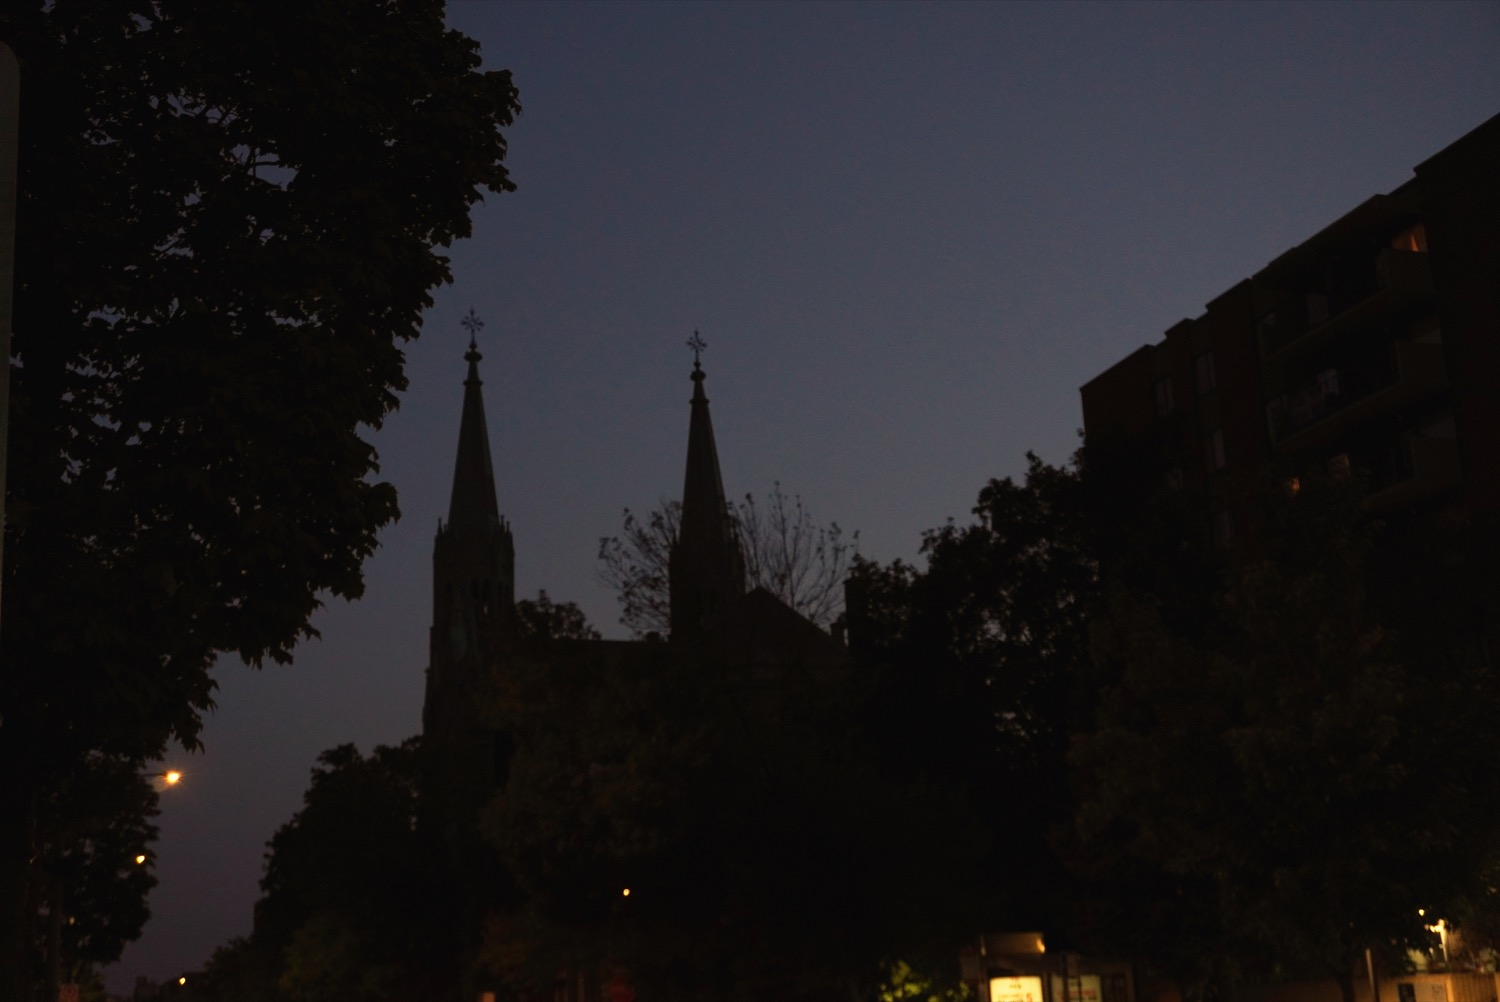
\includegraphics[scale=0.25]{DSC00200_1.JPG}
    }
    \subfigure{
        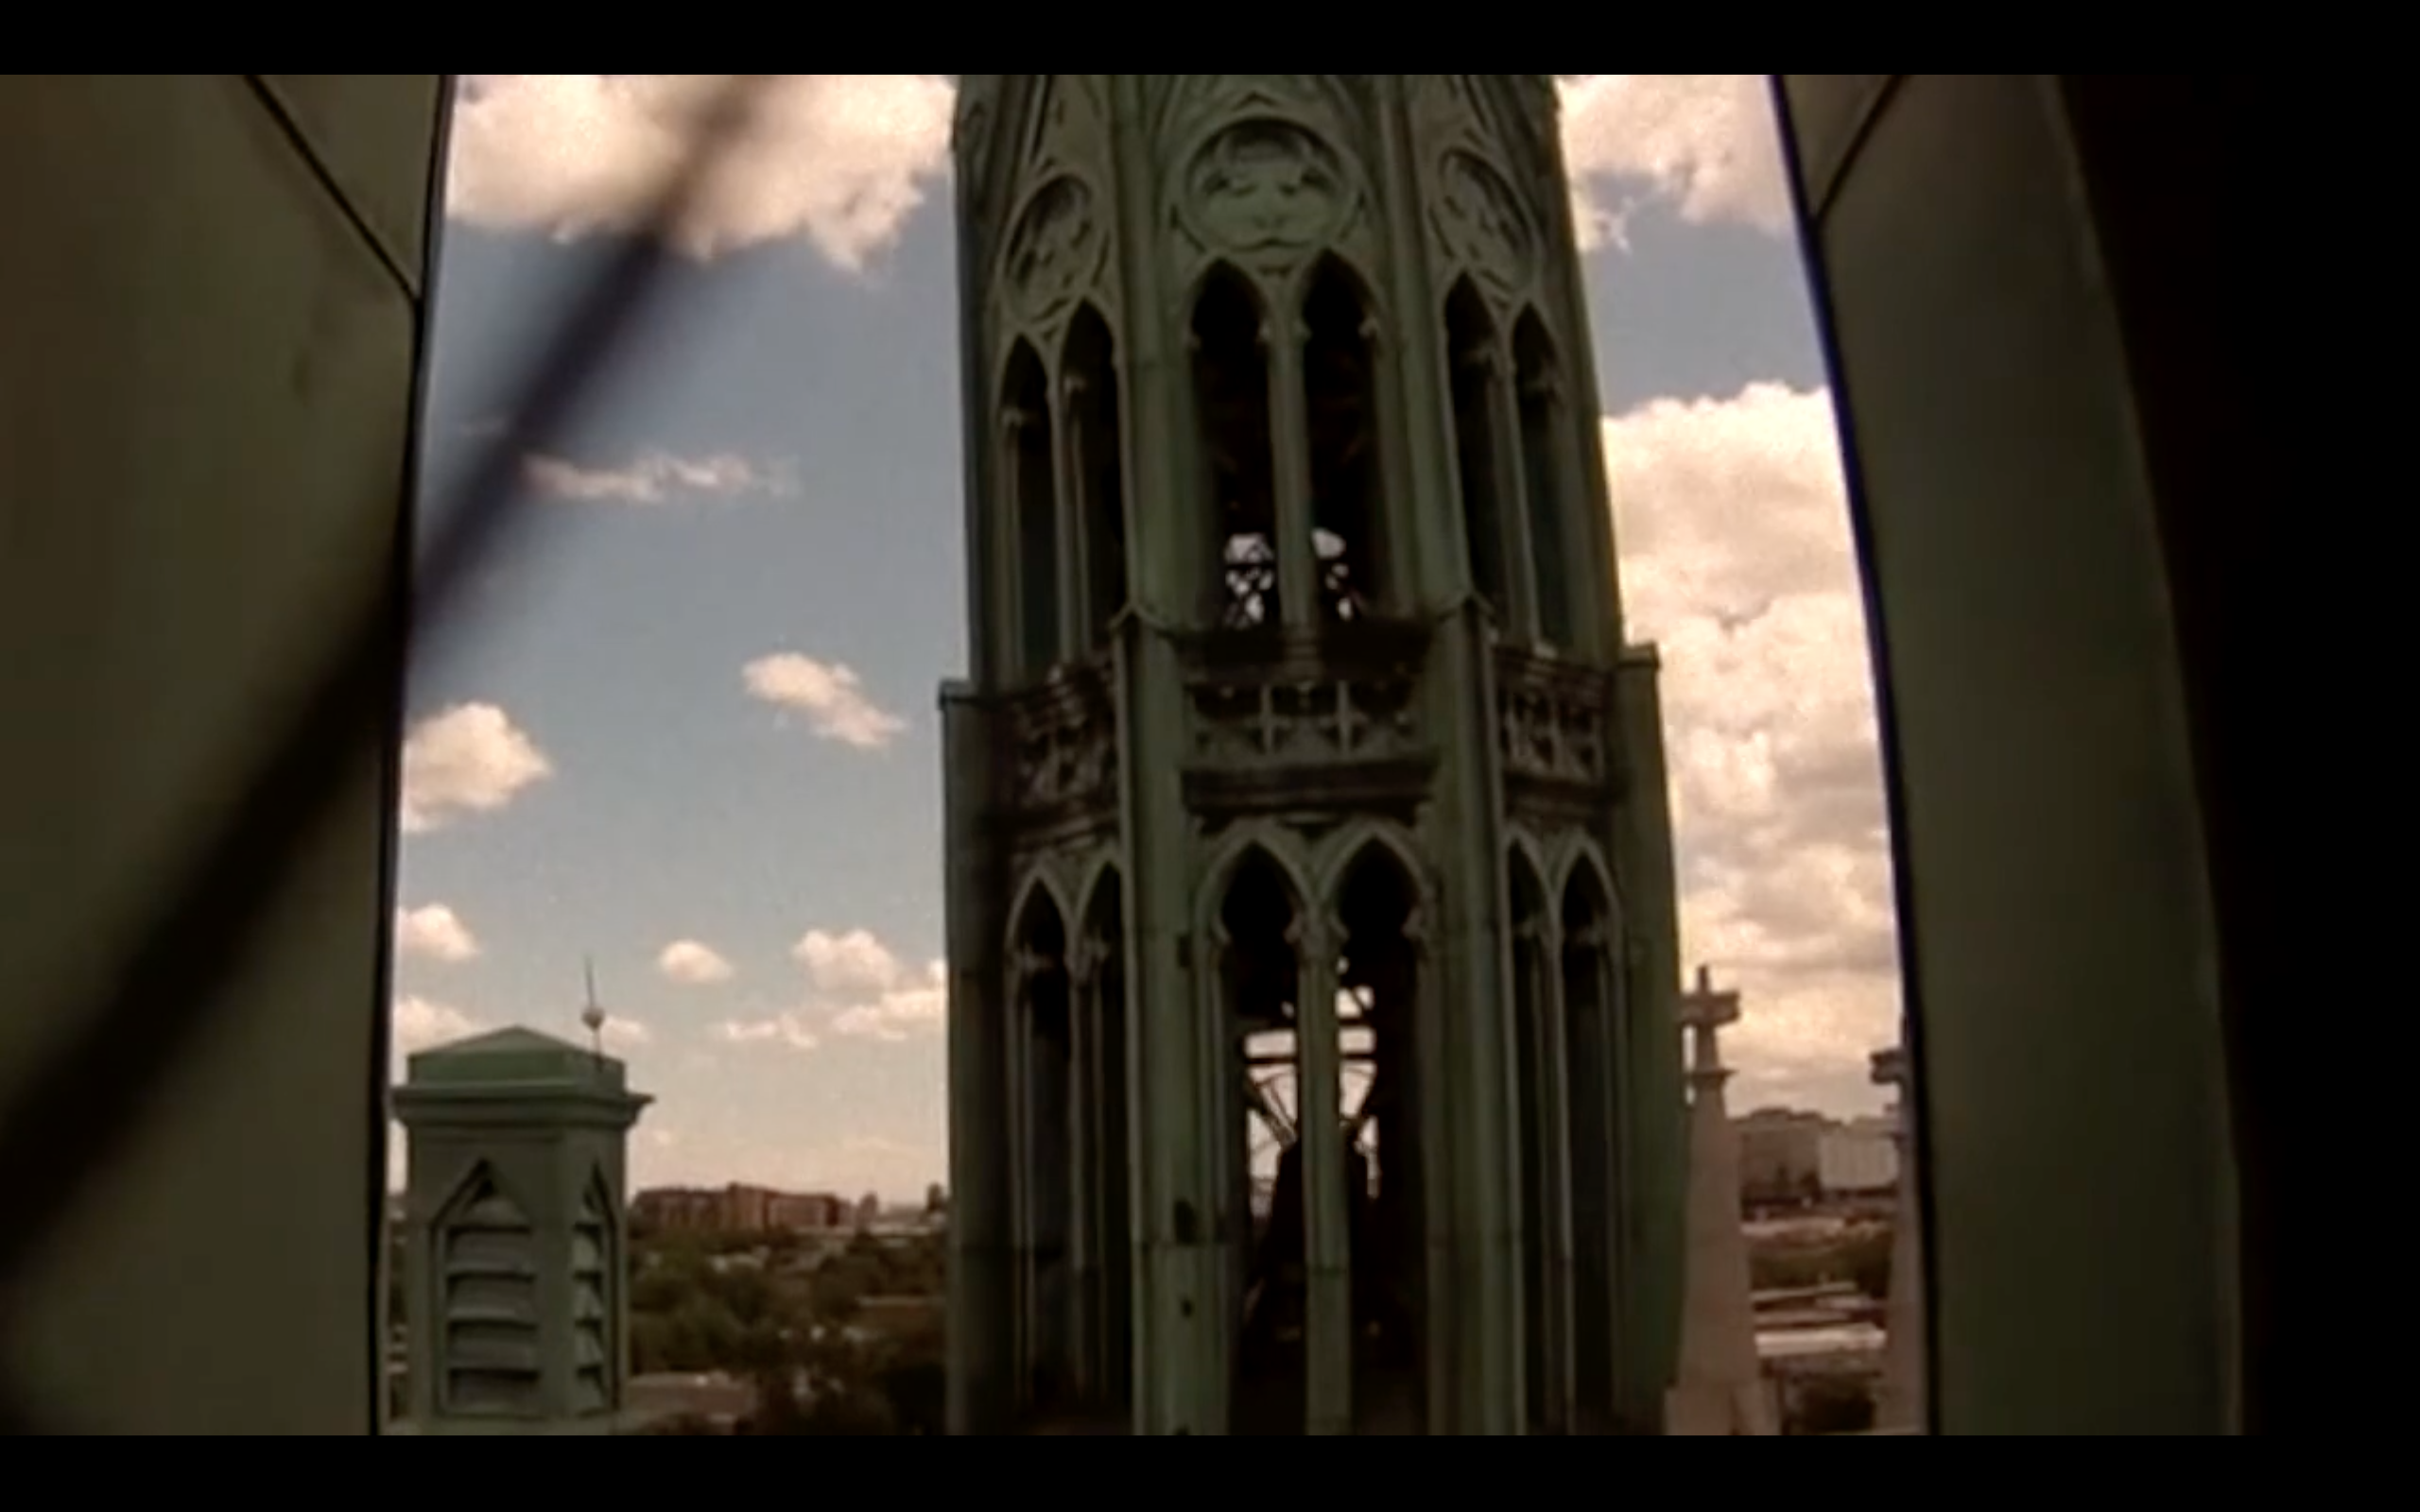
\includegraphics[scale=0.183]{eglise_youtube2}
    }
    \caption{L'église Saint-Édouard from la rue Beaubien on the left, and the footage from the YouTube video on the right.}
    \label{fig:sidebyside}
\end{figure}

The first station opens the piece, and is a combination of two recordings. 
On the one hand, a recording of me walking down Beaubien from my apartment to l'église Saint-Édouard during the summer rain storms of July 2023. 
This is \hl{layered with another} recording that I downloaded from the YouTube channel \hl{\textit{Saint-Edouard de Montréal}} of the bells of l'église Saint-Édouard\footcite{saint-edouard_de_montreal_volee_2022}. 
This latter recording was distorted with \hl{the plugin Chow Tape Model} and treated with the Spectral Blurring plugin by Michael Norris\footnote{These effects become less and less pronounced, to give the impression of a distant sound becoming nearer}. 
These recordings, especially that of the storm, place into question the distinction between inside and outside. 
The church is a contained unit, which is often heavily sonically isolated from environmental sound, especially with stone constructions like l'église Saint-Édouard. 
By using audio recordings from the outside of the church within these confines provides a rare experience of hearing the external from within, as if this sacred boundary had been dissolved.

%%cmt Correction orthographique

\textbf{Second station} (00:06:19--00:06:40):

\customincludegraphics[scale=0.25]{DSC00149_1.JPG}{The sprinkler room upon entering the basement of the church.}%%Station 2

The second station is a recording of entering the church through the basement, and entering the sprinkler room in the basement of the church. 
This is the room that stores all the compressors and valves that connect to the elaborate sprinkler system throughout the church. 
I found that this room emitted an interesting electrical hum, and seeing as it is right beside the entrance on Beaubien, it seemed fitting to begin the journey inside the church at this point.

\textbf{Third station} (00:18:18--00:18:47):

\begin{figure}[h]
    \centering
    \subfigure{
        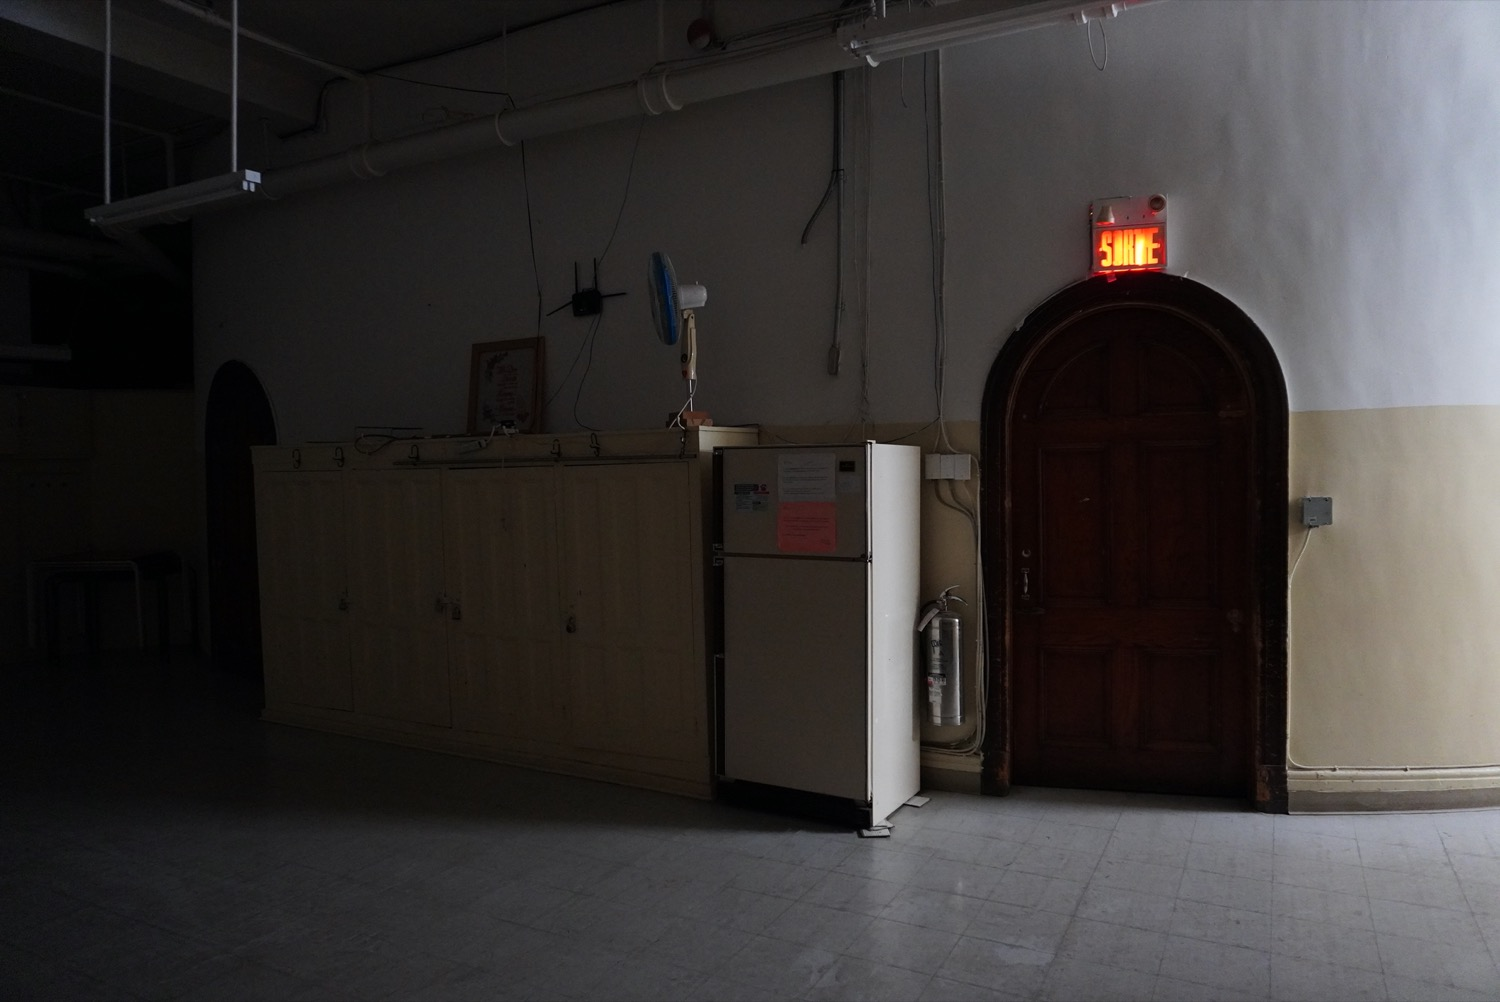
\includegraphics[scale=0.25]{DSC00123.JPG}
    }
    \subfigure{
        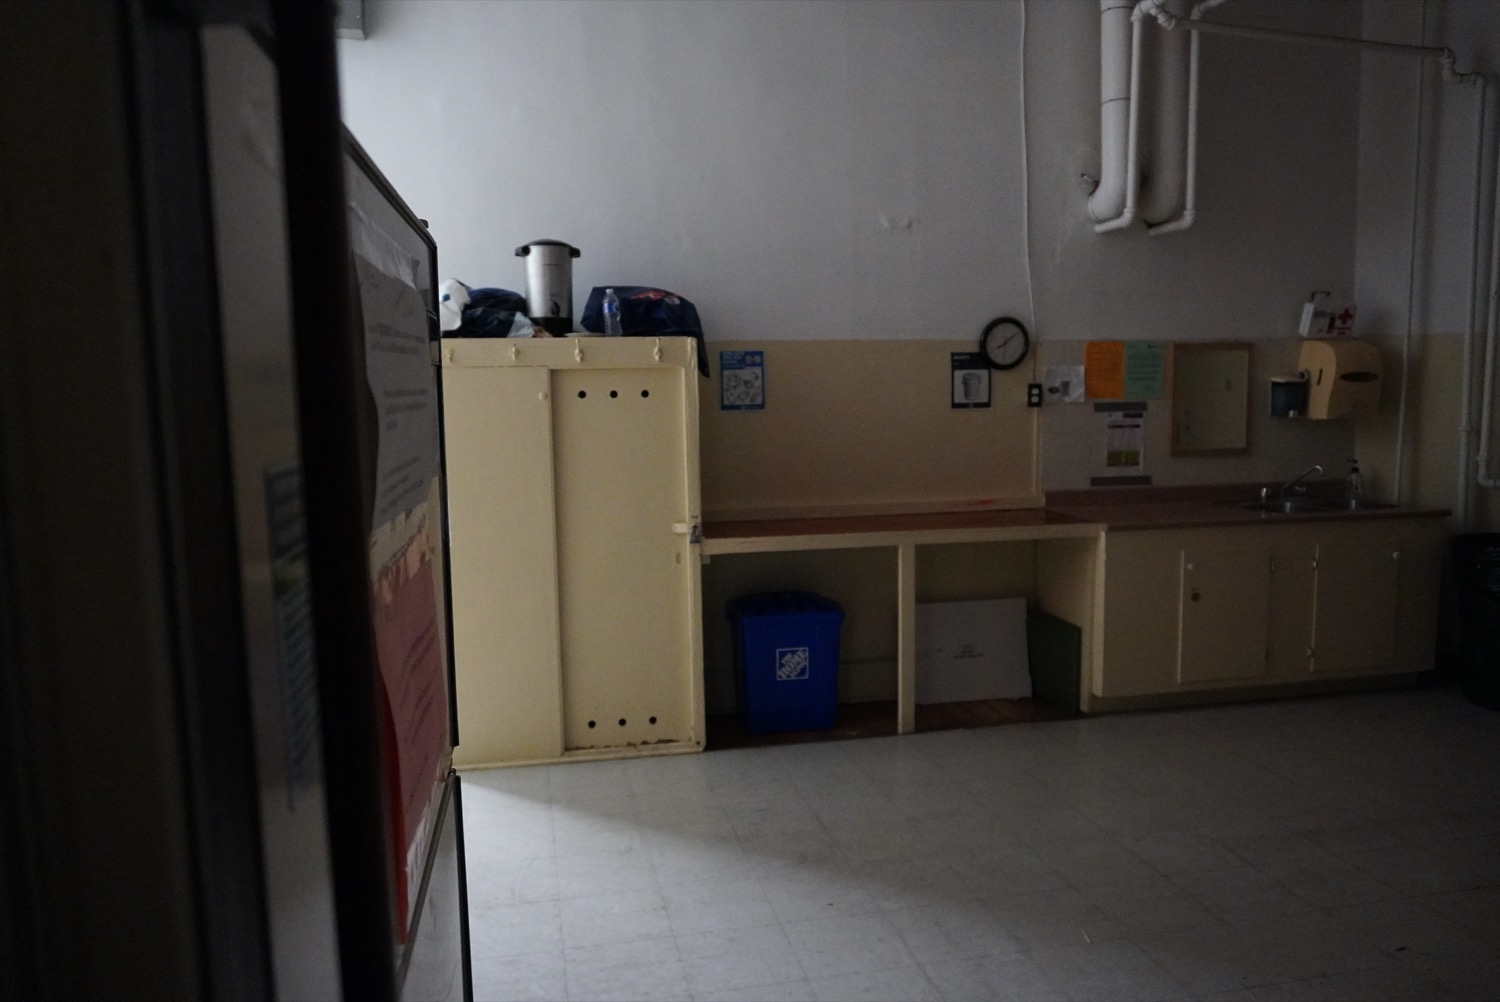
\includegraphics[scale=0.25]{DSC00136.JPG}
    }
    \caption{The fridge of the salle Morin pictured on the left, and the clock viewed from the fridge on the right.}
    \label{fig:sidebyside}
\end{figure}

The third station takes place in \textit{la salle Morin}, a hall that is very frequently rented for events, and is named after the first priest of l'église Saint-Édouard Joseph-Napoléon Morin in 1895. 
This space has two unique sonic features: a dissonantly humming fridge, and a ticking clock. 
Here I play with the unique lens of subjectivity that the microphone provides. 
Elsewhere in \textit{le chemin}, often I am holding the microphone as I walk, providing a close representation of my subjective aural experience, but in the third station, I leave the microphone on the fridge while I leave the room. 
This recording is then crossfaded with another recording where I move the microphone closer and closer to the ticking clock. 
At the same time, I double the sound of the clock, with a time offset, creating the sense of fracturing of time, while my footsteps recede into the distance.

\textbf{Fourth station} (00:27:59--00:43:34)\footnote{Timestamps for fourth and fifth stations are harder to pinpoint as the two are juxtaposed, and elements of each are present throughout a long duration.}:

\customincludegraphics[scale=0.25]{DSC00157.JPG}{The metal sliding door of the furnace room. When the recording took place this door was burgundy, but it has since been painted white.}%%Station 4

The fourth part of \textit{le chemin} begins in the furnace room. 
This room has a fantastic sliding metal door that creates a loud, foreboding sound when opening or closing it. 
This sound opens the seventh movement, which is the only movement that is wholly electroacoustic. 
Furthermore, this is the first time in the piece where two different spaces are juxtaposed. 
By placing the listener simultaneously in the furnace room and in the church, there is a dreamlike, disorienting element, if not directly experienced, as the listener will not recognize the places of recording without prior knowledge, at least at a poetic level.

\textbf{Fifth station} (00:27:59--00:43:34):

\customincludegraphics[scale=0.05]{candles.JPG}{The ever burning candles of l'église Saint-Édouard flicker in the darkness.}%%Station 5

The fifth station marks the entry into the church itself. 
Sonically, this is referenced with three recordings: the sound of a match being struck, symbolizing the candles; the sound of feedback resonance that appeared mysteriously while testing high decay reverberation effects; and the sound of running footsteps that I recorded overtop of this feedback. 

\textbf{Sixth station} (00:43:34--00:47:25):

\customincludegraphics[scale=0.07]{eglise_mh.JPG}{The bell towers whose sound features prominently throughout the piece.}%%Station 6

The sixth station continues the previous station's reference to the opening sounds of the piece. 
Another sample of the July storms of 2023 are heard, this time with an emphasis on the rain rather than the distant thunder sounds featured in the opening bed track. 
Later on, this rain sound is crossfaded into the same bell recording from the beginning of the piece, this time in reverse. 
This reversal of time provides a poignant reference to the theme of transcendance evoked by Rilke's final elegies, while creating a sense of aesthetic unity in the piece.

\textbf{Seventh station} (00:47:55--00:49:10):

\begin{figure}[h]
    \centering
    \subfigure{
        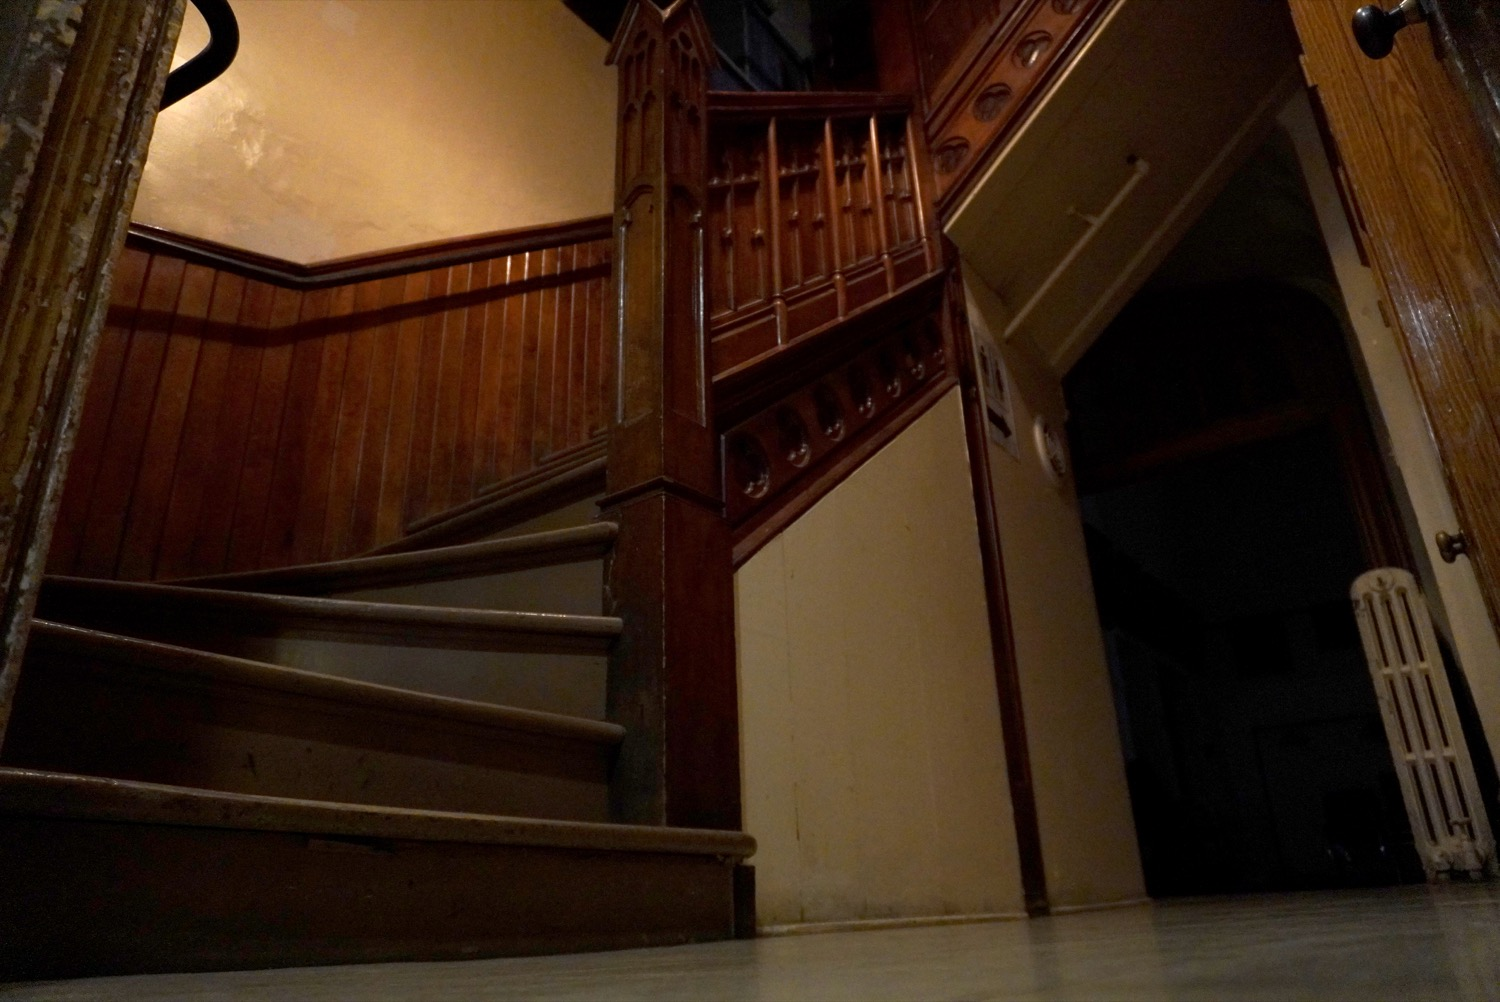
\includegraphics[scale=0.25]{DSC00117_3.JPG}
    }
    \subfigure{
        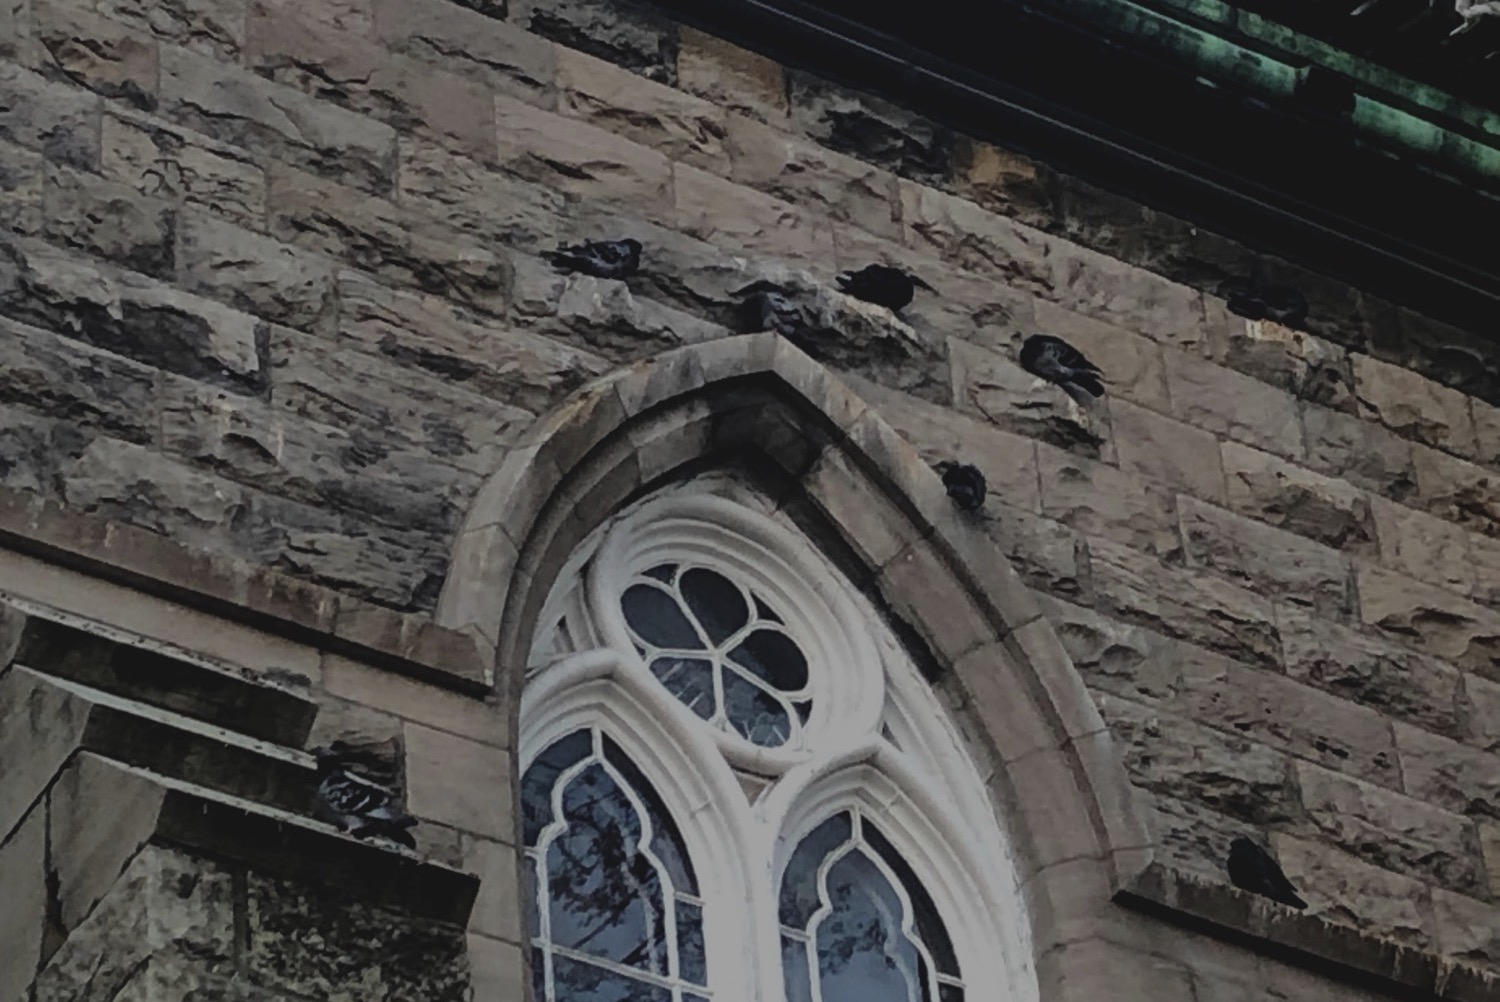
\includegraphics[scale=0.201]{pigeons.jpg}
    }
    \caption{The stairwell leading to the organ loft on the left, and the pigeons of l'église Saint-Édouard nestled into the church's stone walls on the right.}
    \label{fig:sidebyside}
\end{figure}

In the creative process, it is somewhat rare that ideas come in order, and more often than not a major part of this process is organizing the material in a coherent way. 
That was certainly the case with Élégies, with the exception of this final station. 
Not only was this the last part of \textit{le chemin} to be finalized, but the realization of its necessity came only the day before the first performance on April 25, and the recording took place on the morning of the concert itself. 
This station is in two parts, and the first part, the climbing of the stairwell leading to the organ loft, had been my leading idea for how to end the piece for some time. 
It seemed to both symbolize the ascent from the long experience in the depths of the furnace room, which is connected to the organ loft stairwell through what's know as "la mezzanine", but it created a link to the beginning of the piece, which begins by my entering the organ loft from the stairwell. 
In fact, \hl{one} thing that I like about this element is that I imagine the listener to experience the ascent of the stairwell at the beginning of the piece as preceding the beginning of the piece, while after the recording of this ascent featured prominently at the end of the piece, the beginning might be re-interpreted as having started earlier, with the ascent being included as an integral part of the piece.

This idea always seemed, however, sonically lacking. 
The sound of climbing the stairwell in and of itself is not remarkable. 
There is not the same timbral intrigue that the other stations have. 
While preparing for the concert, I suddenly reflected on the first time I had ever seen l'église Saint-Édouard. 
I was walking with my friends Marie-Hélène and Francis, and as we passed the church, admiring it's beauty, Marie-Hélène stopped to take photos of the many pigeons who call the church their home. 
The sound of pigeons is an ever present part of the Saint-Édouard soundscape, and I suddenly realized that this would be the perfect reference to end the piece. 
The sound of the flight of these gentle birds would parallel the ascent of the stairwell, adding to the spirit of transcendence while offering a more interesting timbral profile than the sound of the steps on their own. 
I found an area of the church near a window where the pigeons often sit, and placed my recorder near the open window. 
I left it recording for several hours, waiting for them to arrive, occasionally gesturing at the window to inspire them to fly away. 
I used the sounds of their cooings and flutterings, layered, and gradually slowed down, against the slowed down recording of my footsteps ascending the stairwell. 
Each fluttering is slightly longer, and as the recorder was placed at the middle of the stairwell between the mezzanine and the organ loft, my footsteps gradually become louder before fading off into the distance to end the piece, creating a sense of peace, yet uncertainty, as the footsteps march off to the unknown, leaving the listener behind.

\subsection{Voice}

\hl{Another aspect of \textit{Élégies} that can be grouped under expanded practice is the use of the voice. 
Voice and organ is hardly a unique pairing, but it is unusual for the organist and singer to be the same person.
The centrality of the juxtaposition of the organ and the voice plays a narrative function, placing in contrast two very different paradigms.
The organ as the discrete and technological, with it's distinction between the control interface and the sound production, and the voice as continuous and natural, with the control mechanism and sound production indistinguishable. 
This juxtaposition is eventually resolved.
Initially appearing individually, towards the end of the piece, they are brought together and heard simultaneousy.
This "singing while playing" is typical of other keyboard instruments, but less so with the pipe organ, adding a singer-songwriter element that draws the ear towards more pop oriented references.}

%%cmt Ajout d'une section sur la voix en terme de "Expanded practice"

\section{Aesthetic references}

Here I'd like to outline some of my major aesthetic influences and considerations that shape my approach to making art. 
One of my formative musical experiences was hearing "Everything You Do Is A Balloon" by Boards of Canada on late night CBC radio as a teenager. 
This group's use of archival audio and imagery was my first introduction to music that seemed to be about the past. 
Since then I've discovered other artists who take this approach, especially UK artist Burial. 
His music, especially his first two full length albums, and a 2012 interview with Mark Fisher where he describes his creative perspective, deeply influenced my own \footcite{fisher_burial_2012}. 
In his music, one get's the sense that he's not creating an experience, so much as describing one. 
Rather than the club itself, the sound of the club in the distance, or the memory of it echoing in one's head while walking home. 
Both Burial's attempts to communicate his imagined experience of UK rave culture that he was too young to experience, and Boards of Canada's re-imagining of their childhood in Alberta can be described as a form of hauntology \footcite{alary_vers_2020}.

At the same time that these meditations on the past fascinate me, I've also been influenced by a pursuit of `liveness'. 
The first time that I listened to the music of Arca, for instance, I had the impression of an immediacy---that the music was somehow a living, breathing organism. 
This is a very different approach from the former, and highlights an important tension in my thought. 
I explore this tension through the mixing of live performance and pre-recorded sound files, the combination of what I'll call the organic (the voice) and the inorganic (the pipe organ), and the use of both traditional and modern stylistic references.

Embedded in the question of liveness, especially in a concert context, is the issue of presence. 
Often, performers, instrument designers and composers prioritize clear, comprehensible gestures in order to make the physicality of performance explicitly communicable. 
In my own work, I'm just as interested in the subversion of these expectations, calling into question the nature of shared space. 
By exiting and re-entering the view of the audience, including gestures that do not have a sonic result, as well as sounds that do not have a corresponding gesture, we engage in a play of shadows---a commentary on information loss and incommunicability. 

\section{Tools}

Before entering into the analyses of the work itself, I want to make a brief mention of the various tools that I've used in the construction of Élégies. 
Besides my own software OrganLab, which I mentionned in the previous chapter, I've used several tools to help investigate, test, sonify, and notate my compositional ideas, without which the writing of this piece would be simply not possible. 
First of all, Ableton Live was used not only in a performance context to trigger sound files, apply real-time effects and manage spatialisation as discussed in the previous chapter. 
It also served as an indispensable tool for arranging my improvisations and compositional ideas so that I could envision the macro structure of the work. 
I also used Ableton Live for the sound design of all the bed tracks. 
Reaper was also used to batch slice and export the samples used for the beat towards the end of the piece.

Another essential piece of software was MuseScore. 
MuseScore was used to express my ideas in notational form, allowing me to gain distance from my improvisations and form the material without my physical constraints, leading all the way to the finished score, created with a single .mscx file. 
In order to audiate my ideas, I originally used MuseScore's built in pipe organ sound. 
Eventually exasperated by this wholly uninspiring playback, I investigated alternatives, ultimately discovering Grand Orgue. 
In the summer of 2023\hl{,} I created a custom .organ file for GrandOrgue based on the Burea Church organ, which was made to mimick the both the layout of the stops of the organ at l'église Saint-Édouard, as well as the corresponding stop sounds as close as possible. 
I did this by combining stops that I felt similar from various different virtual pipe organs, creating a frankenstein organ whose stops draw from a wide range of epochs and building styles. 
Eventually, it would be wonderful to sample the stops at l'église Saint-Édouard and create a virtual organ representing this space, but for the purposes of creating MIDI mockups, this was already leagues ahead of MuseScore's built in sounds. 
I followed an excellent Virtual Pipe Organ (VPO) guide by Jester Musician on the MuseScore forums to implement GrandOrgue into MuseScore 3 using a custom instruments.xml file and Staff Text Properties to manage registration changes \footcite{musician_jester_how_2018}. 
I was even able to drive and manage the cues in OrganLab and Ableton Live with this same .xml file. 
Unfortunately, as of my last attempts with MuseScore 4 in early 2024, it still does not support this VPO integration, and so I've been using MuseScore 3 until this is available.

\customincludegraphics[scale=0.3]{grand_orgue.png}{My emulation of the Saint-Édouard organ, mimicking it's console and borrowing stops from several different organs.}

I will make a special mention of OpenMusic for helping me to explore some more technical solutions outside of my cognitive computational ability. 
Though I didn't ultimately implement much of these experiments into the final score, it was nevertheless a useful way to workshop my ideas that I look forward to exploring more deeply in the future.

\chapter{Élégies}

\customincludegraphics[scale=0.5]{2024-04-28_MH_sat50.png}{}

\section{\colorbox{red}{1\textsuperscript{re} élégie}\footnote{00:00:00--00:03:45 in elegies\_video.mp4}}

\epigraph{\textit{Qui, si je criais, qui donc entendrait mon cri parmi les hiérarchies des Anges?}}{}

\subsection{Narrative context}
Rilke's Elegies\footnote{The title of the piece \textit{Élégies} as well as the movement names use french orthography in hommage to the french translation that I used, but I will use the english form in the body of these analyses for ease of reading.} begin not with a cry, but with the question of a cry.
A question seemingly addressed to no one.
A plea of solitude and desperation.
Perhaps this question is addressed to God, to the reader of his poem, or to the protagonist herself.
In any case, this question could be read as an internal cry, representing the subjectivity of our protagonist's lament.
He goes on to evoke the level of solitude felt in his unknown setting, wondering if anyone is listening at all, calling into question the purpose of crying, or of communicating in any way.

From a sonic perspective, the issue of sound is immediately relevant, the cry evoking at once a sound source---the human voice---and the volume, and intensity of this sound.
The subjective nature of sound is also essential, with "qui donc entendrait" illustrating the importance of hearing and perception to the auditory experience.
This startling juxtaposition between the immense loudness of the subject's inner world, and the expansive quietude of the environment provides an immediate dialectic between inner and outer worlds.

The second part of the sentence describes the setting somewhat, though in obscure terms.
He depicts the subject as being among "the hierarchies of angels".
This implies another essential tension to Rilke's world: the spiritual versus the human.
Here is a startling image.
We were quickly led to believe that we were alone, contemplating the futility of communication, when not only are we not alone, but we are found among a cacophonie of angels.
The reason that the angels might not hear the subject's plaintif cry is unclear. 
Maybe the angels are simply too far away.
Maybe they are making too much noise themselves to hear anything.
Or maybe they do not contain the capacity for subjective experience at all.
If we take this last case, this quickly paints an image of Rilke's angel, not as an idealized human, but as a very different creature entirely.
The idea that they would hear nothing implies an austere, cold distance from the angels---the small human alone underneath a swarm of ethereal beings.

\subsection{Materials and techniques}

Software:

One of the main advantages of a digital pipe-organ over an acoustic instrument, is the ability to use non-discrete pitches.
To represent the hierarchies of angels, I thought that it would be appropriate to make use of an extended glissando, starting in a lower register and moving upwards, signifying some kind of transcendental nature.
It might seem strange to represent a hierarchy with something non-discrete and essentially non-hierarchical, but at the same time, the hierarchy is already present elsewhere, such as in the harmonic series, and the strangeness of the glissando evokes something inhuman---alien.

This glissando is not the same that is associated with other instruments. A more appropriate term would be `spectral glissando'. The way that this works, is that over the course of a set amount of time (in this case two minutes), the frequency of each of the eight partials is incremented by one about ten times a second.
Because the frequency is being incremented, and not the MIDI cents, the sound quickly becomes inharmonic.
For instance, if 100Hz and 200Hz are the first two partials, after an addition of 10Hz, 110Hz, and 210Hz are no longer multiples of each other.
This process creates the sensation of an alien movement, pulsating and morphing, yet not in a coherent, familiar way.    

%%cmt Précision de Hz

\begin{figure}[H]
\begin{lstlisting}[language=Python]
glissC = [0 for i in range(8)]
def glissUp():
    global glissC
    for i in range(len(glissC)):
        glissC[i] == 0
    if glissC[0] < 600:
        stop1.setTrans(glissC)
        for i in range(len(glissC)):
            glissC[i] = glissC[i] + 2
    else:
        for i in range(len(glissC)):
            glissC[i] = 0
\end{lstlisting}
\caption{The glissUp function takes a python list and increments it until it reaches 600, this list is used to increment the first 8 partials of the synthesis module}
\end{figure}

Compositional:

For this movement, I wanted to represent the binary form of the poetic fragment with a juxtaposition of proportional notation and semi-metric notation.
The proportional notation is supposed to represent the angelic form.
Here again the choice is somewhat arbitrary.
One could easily make the case that metrical time is more hierarchical.
At the same time, metrical time has a long tail of history in western notation, and has for me a notion of human comprehensibility, whereas proportional notation is newer, with less historical associations.
Furthermore, proportional notation seems to give the sense of music frozen and static in time, which I associate with the timelessness of the ethereal.

\subsection{Form and compositional process}

This movement begins with layered recordings of a walk through a storm and the Saint-Édouard bells, representing the first station of \textit{le chemin}.
This recording is triggered before the performer(s) arrive in the organ loft, either with OSC, or by a helper hidden in the organ loft that can access the MIDI keyboard.  
These sounds enter gradually, building, and eventually looping the final portion to ensure that the ascent to the organ loft is not constrained to a specific time. 
Upon arriving at the organ and verifying that everything is well prepared, the performer simply presses the next key on the midi keyboard, the recording gradually fades out, and a melodic fragment is sung.
This melodic fragment is adapted from a session of singing the poetry of Rilke in l'église Saint-Édouard in the fall of 2022\footnote{This was a solo session where I paced throughout the dimly lit church while searching for melodic material in the text. I recorded these experiments on my Zoom H4N and later sifted through them for the most compelling moments.}, and is developed throughout the rest of the piece.

%%cmt Ajout du contexte sur la séance d'enregistrement

%%\begin{figure}[H]
%%    \centering
%%    \customincludegraphics[width=\textwidth]{1e_1}
%%    \caption{The principal melody of the piece, based on the 19 syllables of the first line of Rilke's elegies (p. 1, sys. 1)}
%%\end{figure}

\begin{example}[H]
    \centering
    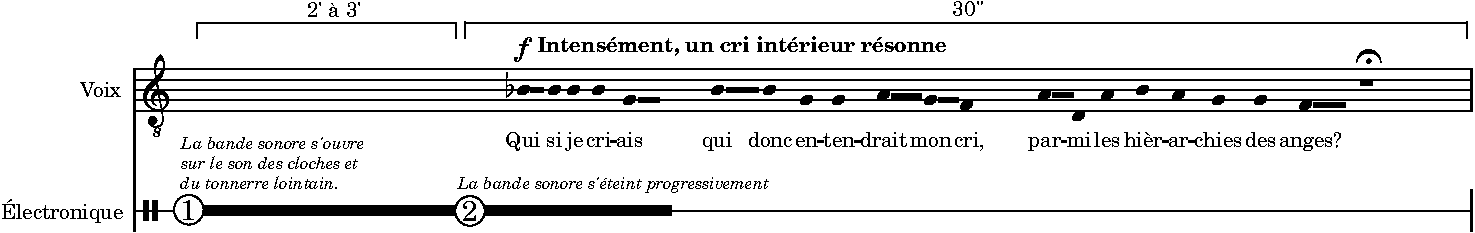
\includegraphics[width=\textwidth]{1e_1}
    \caption{The principal melody of the piece, based on the 19 syllables of the first line of Rilke's elegies (p. 1, sys. 1).\protect\footnotemark}
\end{example}

\footnotetext{In all excerpts in proportional notation, accidentals carry to the end of the system.}

%%\customincludegraphics[width=\textwidth]{1e_1}{The principal melody of the piece, based on the 19 syllables of the first line of Rilke's elegies (p. 1, sys. 1)}\protect\footnote{In all excerpts in proportional notation, accidentals carry to the end of the system.}

I wanted to then create a sonic interpretation of the cry---the internal, subjective cry.
Of course there is no correct, objective way to represent subjectivity, but I've attempted a poetic approach.
To do this, I call upon a characteristically property of the North American pipe organ: the crescendo pedal.
This pedal allows the player to quickly open or close many stops simply by flicking the foot.
One loses detailed control over the registration, yet gains access to a quick dynamic swell that surpasses the capacity of the normal expressive pedals.

This section begins with the crescendo pedal open about \hl{60\% of the way, with the acoustic and digital organs playing the same D minor chord (p. 1, sys. 2).
Just} before playing this chord, the third cue begins the spectral glissando, which is sustained by the sustain pedal.
At first, the acoustic instrument masks the digital sound completely, evoking solitude, but gradually the crescendo pedal closes and the acoustic instrument is masked, leaving the glissando in the foreground.
The gradual widening of registral distance between the acoustic organ and the digital glissando symbolizes the distance between the human and the angelic realms.

\customincludeexamples[width=\textwidth]{1e_2}{The first system of the pipe organ is notated with proportional notation. The sustain pedal is used to maintain the spectral glissando (p. 1, sys. 2).}

Towards the end of the movement, the pipe organ slowly enters with ascending chords built around open fifths and fourths.
These mostly parallel, open harmonies for me evoke two influences.
On the one hand the organum tradition of Leonin and Perotin, and on the other hand, the open harmonies of Boards of Canada.
Ultimately, these chords rise like the synthesized glissando, representing the human caught under the ethereal.
Here the notation changes from proportional, to semi-metrical.
I use this word because the proportions of metrical notation are present, yet without barlines, and rests with fermatas providing flexibility.

\customincludeexamples[width=\textwidth]{1e_3}{Rising chords based on open fifths and fourths (p. 1, sys. 3).}

\subsection{Theatrical and spatial elements}

The theme of theatricality may not be immediately apparent in the opening movements of \textit{Élégies}, yet the ascent to the organ can be seen as a foreshadowing of the increasinly important role that it plays in later movements.
When I project myself as an audience member, I imagine that this ascent, though accompanied by the recordings, would feel more a prelude to the piece than part of the piece itself, especially since the performer is not yet visually present.
In later movements, however, we will see that this issue of presence is called into question.

\section{\colorbox{red}{2\textsuperscript{e} élégie}\footnote{00:03:50--00:06:23 in elegies\_video.mp4}}

\epigraph{\textit{Tout Ange est terrible. Et pourtant, malheur à moi! et pourant je vous invoque...}}{}

\subsection{Narrative context}

I found this poetic fragment to be one of the more difficult to interpret. 
The word terrible, in particular, could be read as ferocious and terrifying, yet could also represent a more subdued pathos, closer to pity.
Rilke then goes on the invoke these angels.
There is clearly a tension implied by the word `pourtant', giving the impression that despite her misgivings, the protagonist nevertheless relies on the angels.
Moreover, there is a sense of regret, as if pride prevents our protagonist from wanting to submit themselves.
They do so in spite of themselves and in spite of the terrible and uncertain nature of their guides.

Ultimately, I chose to emphasis the connotations of pathos and frailty in the word `terrible' with an extremly soft dynamic, and the fearsome quality with a dissonant harmonisation.
This approach attempts to capture the complexity of representing the terrifying nature of the angels, while situating this fear in the mind of the protagonist.
The second part of the movement delves further into this commentary on frailty, maintaining a soft dynamic, this time using a very traditional form of renaissance inspired counterpoint.
For me, this reference to history, and the clear, simple harmonies suggest the human, rather than the angelic.
Here, the protagonist is in prayer---a plea before embarking on an arduous journey.

\subsection{Materials and techniques}

Synthesis:

The use of a gradual dynamic envelope is a pivotal element in this movement.
The traditional pipe organ uses a pronounced, sudden attack, known as the chiff.
In baroque era organs, this chiff is particularily apparent, and while in the romantic era this effect was considerably reduced through a process called nicking, the attack remains very short.
Using the synthetic organ, one can slow this attack as much as they like. 
In this movement, I've chosen an attack of about eighty milliseconds for the transient content, and about six hundred milliseconds for the harmonic content. This is not particularily long, which allows for a contrapuntal clarity, while being long enough to diverge from what one would expect from a pipe organ sound.
Tonally, traditional bourdon sound is modified by accentuating the fourth partial.

\begin{figure}[H]
\begin{lstlisting}[language=Python]
def dynEnv():
    print(`Enveloppe dynamique')
    stop1.setPart([1, 2, 3, 4, 4, 4, 0, 0])
    stop1.setMul([0.588, 0.338, 0.665, 0.773, 0.512, 0, 0, 0])
    stop1.setEnvAtt([0.285, 0.450, 0.327, 0.338, 0.385, 0.277, 0, 0])
    stop1.setEnvDec([0.02, 0.04, 0.085, 0.008, 0.008, 0.008, 0, 0])
    stop1.setEnvSus([0.446, 0.523, 0.404, 0.05, 0.05, 0.542, 0, 0])
    stop1.setEnvRel([0.1, 0.1, 0.1, 0.1, 0.1, 0.1, 0, 0])
    stop1.setNoiseAtt(0.081)
    stop1.setNoiseDec(0.146)
    stop1.setNoiseSus(0.7)
    stop1.setNoiseRel(0.1)
    stop1.setNoiseMul(3)
    stop1.setNoiseFiltQ(3)
    stop1.setSumMul(0)
\end{lstlisting}
\caption{The dynEnv function alters the dynamic envelope of both the harmonic sound and the noise sound, while tripling the fourth partial}
\end{figure}

Compositional:

This movement involves a dissonant harmonization of the main melody, opening with a harmonic structure inspired by the altered dominant chord that is prevelant in jazz traditions.
My variation swaps the typical minor 7th interval for a major seventh.
This chord could also be called a major 7 (\sh9 \fl13), but I tend to think of it in relation to the altered chord.
This harmonisation ends with a minor chord with a \fl6 with a swell, which is echoed in the final movement.

\customincludeexamples[]{g7alt}{A classic G7alt chord on the left, and my variation with a \sh7 on the right.}

Towards the end of the movement, I incorporate an inverted version of the melody incanted at the beginning of the first movement as a cantus firmus in a three voice texture.
This melody begins on F\na\ and represents not a chromatic inversion, but a transposed, diatonic inversion---transposed in the sense that the melody does not begin on the same scale degree as the original (B\fl, the sixth degree of D minor), but instead begins on the third degree of D minor. 
All durations in this voice are equalized as whole notes, and played with the pedals.

\subsection{Form and composition process}

This movement, like the first, begins with the voice.
I considered using new motivic material, but ultimately decided that it would be better to use a variation of the original melody.
This is partly to maintain coherence, and partly in reference to the Magnificat of Jehan Titelouze which uses a repetition of a sung melodic fragment as a formal element.
This thematic variation is now infused with additional chromaticism, reflecting a progression into complexity and uncertainty.

\customincludeexamples[width=\textwidth]{2e_1}{A variation of the sung melody from the first movement, with more chromaticism (p. 2, sys.1).}

My first interpretation of the word `terrible' was the ferocious one, and I chose to open the organ portion of the movement (p. 2, sys. 2) forte, with the dissonant harmonisation striking an unforgiving discord. 
At the same time, I found myself disappointed that the second movement open in the same fashion as the first, with a big loud chord.
From a narrative perspective, it seemed much more logical to open the work with a loud sudden gesture, and then work our way up gradually from the bottom.
Ultimately, I decided to change the opening dynamic to pianissimo, using the dulciane stop, which on the organ at l'église Saint-Édouard is extremely soft.
Being that the chords are still dissonant, this creates an effect of viewing the `terrible angels' from a distance. 
I imagine the protagonist at the bottom of a steep ascent, similar to Dante in the beginning of his journey through hell, while she views the movement of the angels in the heavens.
Perhaps these entities are never seen directly, but only felt from afar.
This section is notated in proportional notation to imbue the harmonic motion with a clouded, murky quality.
I nevertheless attempted to create a sense of voice leading within this dense texture.

In the following section, metric notation is introduced for the first time.
This symbolises a step towards the human, emphasizing the history of western notational practice, as well as a more structured, clearly dilineated rhythmic structure. 
This section uses the cantus firmus as middle voice in a three voice texture, where the bassline is taken by the left hand on the grand orgue division and the treble by the right hand on the MIDI keyboard.
The harmonic language of this section aimed to reference renaissance counterpoint.
This involved careful consideration of the resolution of dissonances, while maintaining a fluid musical dialogue between the voices.
The movement, starting from a D minor perspective, culminates in a half cadence to the A minor dominant.

\customincludeexamples[width=\textwidth]{2e_2}{System showing the progression from dense chromatic harmonies in proportional notation to metrical notation with outervoices braiding an inner cantus firmus (sys. 2).}

The movement concludes with an auditory link to the next---a sound sample of the protagonist opening the door leading to \textit{la salle Saint-Édouard} in basement of the church, representing the second station in \textit{le chemin}.
The mundane, yet eerily resonant sounds of the church's underbelly, including the hum of  the sprinkler compressors, provide a sensory bridge to the third movement.
This mirrors the thematic journey of the music, from the divine to the earth, the celestial to the subterranean.

This recording also serves a practical purpose, this time as linking material between movements. 
I trigger the recording with the attack of the final chord of the second movement, with the hum of the compressors copied and doubled at the fifth below, giving me the E natural to begin the next movement.

\customincludeexamples[width=\textwidth]{2e_3}{The final systems of this movement lead to a half cadence in A minor as an audio recording is triggered (mm. 15-23).}

\section{\colorbox{red}{3\textsuperscript{e} élégie}\footnote{00:06:23--00:10:47 in elegies\_video.mp4}}

\epigraph{\textit{Chanter l'Amante est une chose. C'en est une autre, hélas! de chanter cet occulte Fleuve-Dieu du sang.}}{}

\subsection{Narrative context}

I interpret this poetic fragment as a reflection on the difficulty of walking the path ahead--contemplating the dichotomy between the relative simplicity of singing of love, versus the profound challenge of vocalizing the sacred, yet enigmatic, “God river of blood.”  
This highlights a dialectic between thought and action, and the contrast between superficial perception and embodied reality.  
This narrative conflict sets the tone for the movement's musical exploration.  
Musically, I interpret `chanter', in a few ways, on the one hand, as the voix humaine stop on the récit, with tremolo, which imitates the sung human voice.  
"Chanter l'Amante" is represented by a simple song-like melody, and "Chanter cet occulte Fleuve-Dieu du sang" is interpreted as a compositional and timbral disintegration. 
This movement is situated directly after the second station in \textit{le chemin}, the voice entrance overlapping slightly with the sound of the compressors of the sprinkler room.

\subsection{Materials and techniques}

In trying to complement the voix humaine with OrganLab, I thought it would be appropriate to emulate the tremolo of the voix humaine stop with frequency modulation of a voix humaine emulation in OrganLab.  
With this idea, it seemed like a logical next step to increase this frequency modulation in speed, while changing the index and ratio, such that the natural trembling of the voice, passes through a comic, exaggerated warble, gradually losing the sense of sung tremolo altogether and giving way to an inharmonic, bell-like sound.  
This is all done by interpolating with SigTo() objects, and the entire process takes place over 180 seconds.  
The one part that is not interpolated, due to limitations of ADSR objects in Pyo, is the envelope, which simply changes suddenly at the end of the 180 seconds.

\begin{figure}[H]  
\begin{lstlisting}[language=Python]  
bellCall1 = None  
bellCall2 = None  
bellCall3 = None  
bellCall4 = None

def bell():  
global bellCall1, bellCall2, bellCall3, bellCall4  
bellCall1 = CallAfter(stop1.setEnvAtt, time=180, arg=(.001, .001, .001, .001, 
0.001, 0.001, 0.0001, 0.0006, 0.0007, 0.0005, 0.0006, 0.0003, 0.0005, 0.0003, 
0.0006, 0.0005, 0.0004, 0.0002, 0.0001, 0.0001)).play()  
bellCall2 = CallAfter(stop1.setEnvDec, time=180, arg=(1.3, .05, .02, 0, 0, 0.04, 
.004, 0.04, .04, 0.04, .04, 0.04, .04, 0.04, .04, 0.04, .04, 0.04, .04, 
0.04)).play()  
bellCall3 = CallAfter(stop1.setEnvSus, time=180, arg=(.4, .1, .02, .01, .01, 0.01, 
.01, 0.01, .01, 0.01, .01, 0.01, .01, 0.01, .01, 0.01, .01, 0.01, .002, 
0.002)).play()  
bellCall4 = CallAfter(stop1.setEnvRel, time=180, arg=(2, 0.1, 0.1, .01, .03, 0.4, 
.04, 0.04, .04, 0.04, .04, 0.04, .04, 0.04, .04, 0.4, .04, 0.04, .04, 0.4)).play()  
setInterpol(180)  
stop1.setRamp(180)  
stop1.setMul([1, 0.01, 0.1, 0.01, 0.07, 0, 0.02, 0, 0.01, 0, 0.003, 0, 0.003, 0, 
0.001, 0, 0.001, 0, 0.001, 0])  
stop1.setRatio(0.43982735)  
stop1.setIndex(4)  
stop1.setNoiseAtt(0.001)  
stop1.setNoiseDec(0.1)  
stop1.setNoiseSus(0.01)  
stop1.setNoiseRel(0.1)  
stop1.setNoiseMul(0.9)  
stop1.setNoiseFiltQ(4)  
stop1.setPartScRat(1.02)  
print(bell)  
\end{lstlisting}  
\caption{This function morphes the ratio and index of frequency of modulation, as well as a very slight exponential expansion of the harmonic series on the attack, which creates an additionally inharmonic attack. The envelope is altered after 180 seconds through the bellCall function calls}  
\end{figure}

Interpolation in general was a major goal of this project, and one of my initial ideas was the transition between harmonic organ sounds, and inharmonic sounds.  
This process is semantically justified through the passage from the simplicity of singing of love, versus the reality of singing the God river of blood.  
It is as though the simple dream is interrupted by a descent into a more complex timbral world.

In terms of compositional techniques, to further represent singing, I employed song form \footcite{owens_forms_2003}, starting with an 12-bar melody as the A section.
Instead of completing a larger structure, such as AABA, or ABAB, the A section is repeated incessantly.
This repetitive structure refers to the tradition of theme and variations in the western classical tradition, as well as the blues in black american traditions.  
In this case, rather than focusing the variations on melodic development, they are instead based on tempo and timbral changes. 
Each time the twelve bar melody is heard\hl{,} it is slower, and the sound of the voix humaine is gradually distorted into an inharmonic mass.
This slowing down was inspired by an idea to create an exponential or logarithmic variation, where each variation is a ratio shorter or longer than the previous.

\subsection{Form and compositional process}

The movement begins with an uninterrupted transition from the third Elegy, linked by the bed track at the end of this movement. 
This recording, representing the second station, dies as the third Elegy begins. 
Before completely fading out, the B\na\ of the compressor hum is doubled layered with a transposition of the same sound, giving the voice its starting note (E\na). 
Then, overlapping slightly with the recording, the voice enters with a sung fragment, introducing a lilting melody, rising by thirds and spelling out an E minor 7 chord. 
When the text gets to the part about the God river of blood\hl{,} however, the tone changes abruptly, now descending in a serpentine way, through a chromatic passage ending with a series of alternating ascending and descending thirds, ending on C\na\ (sys. 2).

\customincludeexamples[width=\textwidth]{3e_1}{The sung melodic fragment introducing lilting ascending motive is overlapped with the bed track ending the second movement (sys. 1-2).}

The organ then enters with a similar rising motive, harmonized with perfect fifths below the melody, with a thin, hollow texture of 8' and 2' foundations (mm.1-7).
Throughout this process the tonal center is tenous, first suggesting B minor in the voice, then A minor in the organ, before pivoting towards D minor.  
Various alternatives to the lilting rising motive were tried for the introduction.  
The original intention was to write something that felt like a classic song introduction in the tin pan alley tradition.  
In the end, none of my more elaborate introductions seemed as appealing as the stark simplicity of the original rising motive.

This sets the stage for the entrance of the main motive of this movement (m. 8), a lamenting descending line, beginning on the third scale degree, in this case F, and moving down towards the fifth scale degree.  
This descending line is in stark contrast with the rising motive heard earlier.  
Both the tonal and motivic contrast between the opening sung melody, and the following part create a dissonance, not in a harmonic sense, but in a temporal or symbolic sense.  
The relation between the sung material, and the organ material is not yet clear.  

\customincludeexamples[width=\textwidth]{3e_2}{Organ introduction, referencing the rising motive, but leaning towards A minor instead of B minor, which then leads into the main, lamenting melody at the end of the system (mm. 1-17).}

As for the composition of the descending motive, the first four measures came to me around the same time as the rising motive, around September, 2022, when I first started as organist at l'église Saint-Édouard and started my masters program at l'Université de Montréal.  
Throughout the following months, I found myself adding on pieces to this melody, and finding new variations.  
Once I decided to move in the direction of song form, I tried to crystallize the melody into a version that would fit within the bounds of an 8, 12 or 16 bar section. 
I did this by taking all my motivic fragments and shuffling them around in different orders until I found a version that felt like it had a logical progression.  
In the end, the idea seemed to naturally solidify into 12 bars.

%%\customincludeexamples[scale=0.6]{3e_3}{The original form of the melody of lamentation, with the jazz changes that were ultimately not used.}

The melody begins at about \musQuarter\ = 58, with the acoustic voix humaine in the right hand, accompanied by a rhythmic ostinato in octaves with a plein orgue in the grand orgue. 
Halfway through the melody, it is suddenly interrupted by the doubling of the acoustic voix humaine with it's synthesized reflection, and the pedals taking up the left hand's role of outlining the bassline. 
Just prior to this interruption, the melody is stretched metrically in a non-systematic way, where measures 13-14 would have been simply one (m. 6 in the original 12-bar version). 
This allows time for the organist to trigger the sixth cue, which begins the interpolation process of the voix humaine synthesis, as well as prepares the ear for a change. 
As the synthesis enters at measure 15, the tempo decreases slightly to about 90\% of the original (cca. \musQuarter\ = 58), and the metrical extension of the melody continues, with measure seven of the original melody becoming two measures of 3/4 (mm. 16-17), and measure eight becoming a measure of 4/4 and a measure of 5/4 (mm. 18-19). 

The second entry of the melody in measure 23 is even slower, again at about 90\% of the previous tempo (cca. 
\musQuarter\ = 46), and this time, the acoustic voix humaine drops out, leaving only the synthesis against the bassline in the pedals. 
This time, at the same point precisely halfway through the original 12-bar form as the last interruption (m. 
19), the sustain pedal is held down, creating an increasingly dense spectral mass. 
It is here most of all that the listener is immersed into the timbral morphing process. 
Whereas before, the changes in harmony and rhythm distracted somewhat from the transformation taking place, in this more static structure, the listener hears all the partials shifting, twisting, appearing, and disappearing, as the sound becomes increasingly complex. 
This moment is interrupted, however, by an improvisational section using waves of rapid ascending melodic lines based around \hl{C\sh diminished 7} (p. 5, sys. 2). 
This section is much more chaotic than the previous, and reflects the corresponding chaos in the unstable timbral composition. 
This improvisation comes to an end with a held perfect fifth, G and D, allowing us to continue hearing the transformation more directly. 
Once the transformation is complete, this chord is released, allowing the resonance to subdue. 

Concretely, the 12-bar melody is only heard one and a half times, which calls into question the use of the term `variations'. 
At the same time, I like to imagine that these variations continue in a symbolic or imagined sense. 
For instance, the synthesis server has a limit of ten voices of polyphony, so once the sustain pedal is held in measure 29, there is only room for about two measures before adding new notes will not change the sound. 
At the same time, the performer continues playing the melody, leading to a muted physicality, where the performer is communicating through gesture, but it is not reaching the listener. 
The performer could very well continue playing this silent melody, and from a listener's perspective, I can imagine myself trying to find the melody lost in the thick fog. 
In this sense I see the second variation not so much being interuppted, but covered. 
In fact, the improvised section, though bearing little resemblance to the original theme, could be considered the third variation.

After the arrival of the bell sound at the end of the transformation, the bells then sound three times a rapid descending line, ending with a powerful strike of an open fifth in each hand, allowing for each to decay. 
These three tolls of the synthetic bells signal the end of the movement. 
The 7th trigger is then initiated, beginning a slow crossfade from the bell sound to the sound of singing glasses, and the fourth is ready to begin.

\customincludeexamples[width=\textwidth]{3e_4}{The end of the second variation, an improvisational section, and the three synthetic bell tolls that end the movement (m. 26 to p. 5, sys. 2).}

\section{\colorbox{red}{4\textsuperscript{e} élégie}\footnote{00:10:50--00:18:48 in elegies\_video.mp4}}

\epigraph{\textit{Vous, Arbres de la Vie, oh! quand donc hivernaux? Nous n'allons pas à l'unisson.}}{}

\subsection{Narrative context}

On the one hand, this poetic fragment speaks to the trees of life.
The object that these trees symbolize is not clear.
Are they the angels, the readers of the poem, or perhaps life itself?
In any case, the poem then places the trees in the inevitability of the impending winter.
This winter can be read as an intimation of death, or at least a dormant state.
The musical term \textit{`unisson'} and its deliberate negation in the next sentence express a sense of divergence or disharmony, which becomes a central theme in the musical interpretation.

From a musical standpoint, I wanted to set the listener in the winter, which for me entails a sense of space and vastness, of stillness.
To evoke this environment, I thought it would be appropriate to use sounds with slow attacks and decays, and decided to make use of the sounds of singing wine glasses.
This also presents a pun, as the french word for ice is glace, which is a homophone with glass, the material of the wine glasses, evoking the ice covered ground of the desolate winter landscape.
This is the first and only time in Élégies when a sound other than the sung voice is used monophonically. This increases the sense of solitude, and in a way can be thought of as an interiorized voice.
As far as the second part of the poetic fragment, I decided that this would be a good moment to bring back the glissando motive from the first movement, this time moving in contrary motion, refering to the text “Nous n'allons pas à l'unisson”.

\subsection{Materials and techniques}

In this movement I make use of sampling for the first time, in two senses.
In one sense, I use a sampler VST in Ableton Live which uses recordings of wine glasses recorded in my apartment.
I had been writing a choral piece called Jardin de Givre, which made extensive use of singing wine glasses, and thought to myself that it would be fun to play these sounds with my keyboard, only later realizing the thematic relevance with the fourth elegie.

On the other hand, I have a longer sample that is not played instrumentally, but is triggered by the smaller midi keyboard, acting as a bed track to support the climax of the movement. The content of this bed track is a recording of me playing an ostinato arppeggio based on the the ascending thirds motive on the organ, which was transposed down by a perfect fifth, originally in order to conform to another section that was in C minor, rather than the original G minor of the sample. I liked the spectral effect of this transposition so much, however, that I decided to integrate it into the piece itself. Later on in the bed track, a recording of the spectral glissando effect in pyo is revisited, this time with the even partials higher in pitch, and the odd partials lower in pitch, essentially exploding the harmonic series into an inharmonic mass. Originally I wanted to play this spectral glissando live, but integrating it with the physical and musical limitations of the musical material was not obvious, and as I was already using the bed track, it was a logical solution to incorporate the glissando in this way.

\begin{figure}[H]
\begin{lstlisting}[language=Python]
def glissCont():
    global glissC
    for i in range(len(glissC)):
        glissC[i] == 0
    if glissC[0] < 600:
        stop1.setTrans(glissC)
        for i in range(len(glissC)):
            if i % 2 == 0:
                glissC[i] = glissC[i] + 0.4
            else:
                glissC[i] = glissC[i] + -0.4
    else:
        for i in range(len(glissC)):
            glissC[i] = 0
    print("0", glissC[0])
    print("1", glissC[1])
\end{lstlisting}
\caption{The function glissCont defines a glissando where each even partial is gradually incremented, whereas each odd partial is gradually decremented. This function is later called by a Pattern object 10 times a second}
\end{figure}

Another bed track is incorporated at the end of this Elegy, this time representing the third station in \textit{the chemin}, as we pass through \textit{la salle Morin} in the basement of the church. We hear the humming of the fridge with a clock ticking in the distance, as the ticking becomes louder, and fractions into several offset ticks, the sounds of footsteps fade into the distance.

\subsection{Form and compositional process}

Unlike all the previous movements, this one does not begin with a sung fragment. The reason for this is that in order for the transition between the bell-like sounds of the end of the third movement and the wine glass sound of the fourth movement to be effective, I didn't want to interrupt it with the voice. Also, from a poetic standpoint, the voice seemed at odds with the desolate landscape that I wanted to represent.
This movement begins instead with an evocation of winter's vast stillness through long, monophonic singing glass samples with gradual attack and decay, unachievable on a traditional pipe organ (systems 1-4).
These melodies are particularily centered on different combinations of the minor third, referencing both the initial melody and the ascending motif from the third movement.
These minor thirds are explored and combined with other intervals to form a fairly free and wandering section with ambigous tonality.

\customincludeexamples[width=\textwidth]{4e_1}{Free monophonic section, using singing glass samples with long attacks and decays (sys. 1-2).}

This melody uses proportional notation to add to the metric freedom of the evolutive sounds. Later, a meter is introduced, and a section of shifting meter (mm. 1-22) gradually finds the nebulous tonality center around C minor.
The introduction of an ascending triad motive ostinato in C minor follows, first slowly, played in the right hand with the singing glasses and accompanied with the bourdon and the pedal. Then in measure 29, a modulating version of the melody of lamentation is introduced in G minor, this time with the melody taken by the bourdon as well, making its way back to C minor before a sudden entrance of the grand orgue division with all keyboards coupled (m. 45), reiterating the same ascending arppeggiation. This motif is heard once more, this time with a light \hl{8'/2'} coupling, before winding down with a chain of suspensions in the right hand while triggering a sound file (trigger 8) with the left (m. 56). This sound file is originally triggered with heavy reverb and an EQ plugin blocking much of the high end. During a thirty second pause of no organ playing, two more triggers are cued, the first of which turns off the reverb effect, and the second turning off the EQ. Both of these triggers restart the sound file in addition to bypassing the effects, and make the initially subdued sound more rhythmic, bright, and impactful. 

\customincludeexamples[width=\textwidth]{4e_2}{The transition from proportional to metric time (sys. 4 to m. 11).}

\customincludeexamples[width=\textwidth]{4e_3}{Entry of the accompanied rising thirds motive (mm. 23-28).}

Then, the sound of a low bombarde sounding a G in the bed track signals the entry of the organ, beginning with G minor arpeggios in the left hand (m. 58). This can be considered an extended version of the rising thirds motif with diminution. 
The arpeggiations also form, both visually in the score, and sonically, a set of arches, symbolizing of the arches and spires of l'église Saint-Édouard.

\customincludeexamples[width=\textwidth]{4e_4}{Triggering of bed track and entry of the arch theme (mm. 53-59).}

Then, a descending melody enters in measure 60. 
This first notes of this melody are reminiscent of the melody of lamentation, this time with each duration equalized to the whole note, and beginning on the first scale degree, as opposed to the third. 
This is the first time in the piece that these two elements are heard simultaneously. 
This melody is heard twice, the first time lasting seven measures, and the second time eleven. 
The crescendo pedal is used strategically throughout this to create large-scale dynamic waves, swelling and fading before and after the melodic lines. 
At the end of the second melodic line, however, this pattern is disrupted, and the crescendo pedal cuts out all at once with a subito piano. 
At the same time, the left and right hands drop out, while the right hand shoots over to strike the next electronic cue (trigger 11). 

This recording also provides a link between movements, this time between the fourth and fifth. 
The recording is triggered at the peak of a dynamic swell as the left and right hands drop out leaving only the sound of the buzzing fridge of \textit{la salle Morin} and the ticking of a clock in the background. 

This begins the third station (p. 12, system 1), which is accompanied by the pedals playing a G. 
Overtop of this soundworld, the sung text "Vous Arbres de la vie. Oh quand donc hiverneaux." accompanies the organ for the first time in the piece. 
The semitone ascent of the melody with the word "Oh" is supported by the pedals, which maintain both notes at once, causing a rumbling beating effect as this dissonance is held. 
The clock ticking becomes louder and louder, and with the final click the, movement is over, moving directly into the fifth.

\customincludeexamples[width=\textwidth]{4e_5}{The poetic fragment set over held pedal tones and a recording of \textit{la salle Morin} (p.12 sys.1).}

\section{\colorbox{red}{5\textsuperscript{e} élégie}\footnote{00:18:50--00:24:40 in elegies\_video.mp4}}

\epigraph{\textit{Mais les errant, dis-moi qui sont-ils, ces voyageurs fugaces?}}{}

\subsection{Narrative context}

The fifth Elegy dwells on the fleeting nature of life and the enigmatic journey of the soul. The fragment that I selected from the beginning of Rilke's poem speaks of wandering souls, asking who they are. One is struck by the nameless, faceless nature of this description. It calls to mind the river Styx of Greek mythology, where the perilous boat crossing is often depicted as being surrounded by phantom souls which float aimlessly. This movement is situated between the third and fourth stations of \textit{le chemin}, as we are moving from la salle Morin towards the furnace room. 

Narratively, this point in the poetry is the hardest for me to define. In a sense, it seems to erode the boundaries necessary for a clear definition. Musically, I represent this obscurity in various ways. On the one hand, a densely chromatic melodic theme is featured, mirroring the winding, unpredictability of smoke. The music is evolutive, with an emphasis on slow transformations and morphing. This creates a nebulous effect evocative of the \textit{voyageurs fugaces} mentioned by Rilke. 

The ticking of the clock in the bed track leading up to the fifth movement also provide an important context. The reference to time, especially as the ticks are gradually doubled and offset, creates a sense of fractioning of time. Combined with the play of subjectivity as the footsteps recede from the microphone for the first time, this appropriately establishes the tone for the liminal nature of the fifth movement.

\subsection{Materials and techniques}

Synthesis:

In the origins of this project was a fascination with interpolation.
I find it very intriguing to take a sound that seems permanent, stable, fixed in place and historical context, and to transform it into something else.
This capability is one of the key advantages afforded to the use of digital synthesis.
A traditional pipe organ operates in a very binary fashion, and this is especially true of electro-pneumatic organs, in which pulling a stop simply sends a control voltage to open the valve to the rank or ranks in question.
Moreover, even with a tracker organ, where half stops exist and are exploited in some experimental music, they are not so much an interpolation of the timbral space of that stop and silence, but are more like a distortion of the normal register, much like overblowing a flute.
This is not to speak of the idea of morphing from one stop to another.
In order to do this with a traditional organ, one would need to transform the metal in real time.
It is simply not possible!

In the digital world, sound is not linked to physicality in such a direct way.
The loudspeaker opens us up to much more flexible ways of generating and manipulating air pressure waves.
Once I had developed my first iteration of the sound synthesis server in python, one of the first ideas that I wanted to try out was this idea of morphing between stops, as if the metal is being stretched or contracted in realtime.
There's not necessarily an objective way to go about doing this, and the most obvious solution would simply be to use a crossfade, making one stop quieter while another enters.
This would be akin to increasing the transparency of one photo while another increases in opacity.
I considered this approach, and when this visual analogy came to mind, I imagined another possibility, where each pixel moves to where it needs to be for the transformed state.
Technically, this doesn't really make sense, as it would necessitate that both the original and transformed image have the same collection of pixels, but in a different order, which would likely not be the case.
In reality the more appropriate analogy would probably be that each pixel stays exactly where it is, but gradually alters it's RGB values until it reaches the desired state.

In any case, this visualisation gave me the idea to manipulate the timbral space itself for my transformations, using the spectral profiles of each stop, and in particular the amplitudes of each partial, as my pixels--a sort of data primitive which can be morphed as needed.
I had already designed functions which instantiated the profiles of different stops.
The only functionality missing was to define a way to interpolate between these states.
After some research, it seemed that the most straightforward approach would be to replace the Sig() objects with SigTo() objects.
The former generates a constant value, and jumps to a new value when changed, whereas the latter object takes a second argument, that of time, which determines the rate at which it moves to a new value once set.

\begin{figure}[H]
\begin{lstlisting}[language=Python]
for i in range(len(part)):
    self.amps.append(SigTo(mul[i], time=self.ramp))
    self.att.append(SigTo(att[i], time=self.inter))
    self.dec.append(SigTo(dec[i], time=self.inter))
    self.sus.append(SigTo(sus[i], time=self.inter))
    self.rel.append(SigTo(rel[i], time=self.inter))
    self.envs.append(MidiAdsr(self.note[`velocity'], attack=att[i],
    decay=dec[i], sustain=sus[i], release=rel[i], mul=self.amps[-1]))
    self.part.append(SigTo(part[i], time=0.2))
    self.snds.append(Sine(freq=(self.part[i]**self.partSc) * 
    (MToF(FToM(self.note[`pitch']-0.15))) + Randi(-rand, rand, 5) + 
    self.trans + self.mod, mul=self.envs[-1]))
    self.mixed.append(self.snds[-1].mix())
\end{lstlisting}
\caption{This snippet from stop.py uses SigTo() objects to manage interpolation between values.
self.ramp is used to determine the rate of transformation of the amplitudes of the harmonics, and self.inter, short for interpolation, governs the changes between envelope parameters.
For the moment self.inter is not functional, due to MidiAdsr() not allowing live signal for it's parameters (the first value is used at instantiation).} 
\end{figure}

This way of spectral morphing can work well at both large and small time scales.
The former giving a sense of evolutive expansion or contraction, depending on whether the spectrum is brightened or dampened.
The latter has a more elastic effect, as if the sound is a physical object and bounces like a rubber ball.
For this movement, I wanted to automate the morphing process, while experimenting with a range of medium time-scales.
To do this, I drafted a function called stopInter() which simply draws a number between zero and three, at an interval between 1 and 10 seconds.
This number represents the bourdon 8', principal 8', voix humaine 8', and cornet 5Rgs.
stops.
Each time a new time interval is selected, the ramp is changed accordingly, creating a sense of spectral instability and constant shifting, like the smoke of our `voyageurs fugaces'.

\begin{figure}[H]
\begin{lstlisting}[language=Python]
stopInterPRand = Sig(1)
def stopInter():
    global stopInterPRand
    x = randint(0, 3)
    stopInterPRand.value = randint(1, 10)
    stop1.setRamp(stopInterPRand)
    print(x)
    if x == 0:
        bourdon()
    elif x == 1:
        principal()
    elif x == 2:
        voixHumaine()
    elif x == 3:
        cornet()
    print(`stopInter', stopInterPRand)

stopInterP = Pattern(function=stopInter, time=Sig(stopInterPRand))
\end{lstlisting}
\caption{The function stopInterPRand interpolates between the spectral composition of the bourdon, the principal, the voix humaine, and the cornet.
The pattern stopInterP triggers the function at a randomly chosen time interval between 1 to 10 seconds.
The interpolation is five seconds long, which is defined in the midi\_nav.py file (see GitHub respository).}
\end{figure}

Compositional:

The use of the word \hl{\textit{fugace}} in the poetic fragment strongly suggests the traditional form of the fugue. 
This realization struck me well into the conception of this piece, long after the idea to use interpolation to represent the nebulous, smoky evocations, and presented several technical challenges. 
In some sense, these two ideas are completely opposed. 
The interpolation idea was fundamentally ambient and evolutive, whereas the fugue has historically featured clearly defined rhythms and melodic motives as a key element. 
Moreover, the interpolation works best with the sustain pedal depressed, and with a wide spread of intervals, to create an immersive resonance, but the fugue theme, which naturally sprung from the text, is tightly weaved and chromatic. 
I'll delve into my creative solution to this problem in the following section.

\subsection{Form and compositional process}

In the construction of the fifth movement, I was sitting before some strikingly varied material, each representing a strong poetic proposition. 
On the one hand, the slow, ambient evolutions of the spectral interpolation, and on the other, the integration of the fugue. 
The stop interpolation had come earlier on in the process, and before exploring the fugal idea, I had already recorded several promising improvisations using this mutation. 
Originally, my idea was to make the entire movement into a fugue, beginning somewhat normally on the acoustic organ, and then having certain fragments of voices taken up by the synthesizer, with the pedal held. 
I imagined this effect as resisting the relentless motor of the fugue, gradually blurring the lines, such that as the synthesizer takes more and more space in the fugue, the entire process dissolves into the nebulous mass.

There were several major problems with this approach, however. 
At a practical level, it is not easy to constantly switch between keyboards while managing fugal polyphony, not to mention while adding a sustain pedal into the mix. 
Secondly, the fugal material wasn't ideally suited to the evolutive texture. 
I found that the stop interpolation sounded the best with wide harmonic intervals and long note durations, whereas the fugal material was tightly chromatic and relatively fast. 
I considered using octave displacement, a technique used by Olivier Messiaen in the sixth movement of his Messiaen’s Vingt Regards sur l’enfant Jesus for piano. 
In theory, this technique, combined with augmentation, would allow me to transform my fast chromatic melodies into slow, widely spaced harmonies. 
At the same time, this was intimidating a the level of composition, and even \hl{more so} from the perspective of a player.

I considered abandoning one of the ideas to concentrate on the other, but then it occured to me to simply place the ideas beside \hl{each other} rather than integrating them intrinsically. 
Originally I imagined the fugue coming first, simply because the voice seemed to naturally signal the beginning of a fugue, which traditionally begins with a statement of the theme. 
At the same time, I was frustrated, because the synthesized material seemed to perfectly capture the mood for the beginning of the piece.

I was at an impass with this movement until the thought came to put the fugue at the end. 
I had nearly finished the fugal exposition, and I began to like the delightful strangeness of finishing the piece with an exposition. 
This subversion of traditional expectations, where the exposition always sets the stage for future developments, seemed an appropriate choice for the wandering, moving forwards while looking backwards souls of Rilke's poetry. 

Once I had this thought, it was only a matter of stitching the elements together in a coherent way. 
After the voice enters with the chromatic melody, beginning precisely with the final tick of the bed track concluding the fourth movement, the player cues the twelfth trigger, which serves a double role, beginning the stop interpolation (with a delay of several seconds to ensure that the first chord is a bourdon sound), and triggering a bed track. 
This bed track is itself a recording of stop interpolation, taken in the church, and was created to serve both as a bridge between the evolutive and fugal section, as well as to accompany my exit from the organ at the end of the movement. 
The harmonic choice was difficult, because it needed to both sound like the continuation of the evolutive section, while appropriately accompanying the fugal section, and not covering it. 
My solution to this problem was to use higher pitches, so that it didn't interfere with the other notes of the fugue (especially the bass line), instead acting more as an integrated spectral component to the sound mass. 
I selected pitches from the end of the evolutive section, while avoiding notes that would be too much in conflict with the F minor/C minor orientation of the fugal section.

\customincludeexamples[width=\textwidth]{5e_1}{The chromatic melody that opens the fifth Elegy and serves as fugal theme (p. 12, sys. 2).}

\customincludeexamples[width=\textwidth]{5e_2}{The opening to the evolutive section using stop interpolation (mm. 1-11\hl{)}.}

The bed track continues to play, though as a background element, while the fugal section begins with the bright sound of the cornet. I often use this stop to introduce the psalm melody during masses, and to me, it evokes thick incense-filled air. It is considered a mixture stop, and it's bright nasal tone has a ceremonious, mysterious quality. Several voices enter the fray and eventually the cornet is dimmed with the closing of the récit's expressive box, while the positif's box is opened, giving more emphasis to the melodie stop. This is a technique that I learned from composer and organist Matthew Lane, and represents the closest analogue version of spectral morphing that I can think of with the pipe organ. The fugue continues to build, until a five voice texture comes to a climax, referencing the lamenting theme with a coda, and then suddenly backing off to a small cluster.

\customincludeexamples[width=\textwidth]{5e_3}{The end of the evolutive section and opening of the fugue exposition (mm. 12-22).}

\customincludeexamples[width=\textwidth]{5e_4}{The first appearance of analogue spectral morphing through alternating expressive pedals (mm. 28-32).}

At this moment there is a short improvisational section, where rather than improvising notes, the same chord is held while the pulling and removal of stops is improvised, as well as continously morphing using the same alternating expressive pedal technique described earlier. After about thirty seconds of this. The former stops, and leaves the organ, holding a flashlight at chest level while slowly crossing the organ loft and out of sight of the audience. Ideally if this is timed correctly, the bed track continues to play, now with lower frequencies introduced, while the player performes their exit.

\customincludeexamples[width=\textwidth]{5e_5}{This movement ends with aleatoric stop selection while alternating expressive pedals (mm. 49-50).}

\section{\colorbox{red}{6\textsuperscript{e} élégie}\footnote{00:24:57--00:27:18 in elegies\_video.mp4}}

\epigraph{\textit{Figuier, depuis longtemps déjà ce m'est un signe que presque entièrement tu te dérobes à la gloire des \hl{fleurs}...}}{}

\subsection{Narrative context}

To me this is the crux of Rilke's texts, and the key narrative moment of the piece.
It is like the voice of God acknowledging that the subject is not living up to their fullest potential, that they are shrinking before the greatness of their task.
It is the point in the story where the protagonist must face his mortality, questioning the possibility of continuing, feeling crushed under the weight of burden, as a small fragile child.
For this movement I wanted to make use of what I call the dissociated bourdon.
In this synthesis patch, the harmonic content, and the transient noise content (marking the attacks of notes), are treated independently, where the noise sounds on every note onset, but the harmonic content sounds every sixth onset.
This creates an effect which is haunting and fragile--largely rhythmic.
The sound world is based in F minor, which refers to the minor triad contained in the harmonics of the spectral analysis of the lowest bell of l'église Saint-Édouard, and fragmented bursts of sound are heard interspersed with the clicking of the transient sounds.
Interestingly, there would have been a fuller contrapuntal message, but it is truncated, hidden, and lost to time.
This is a metaphor for the fig tree, hiding itself and dissociating from its truer form.
For this movement, I thought it would be appropriate to leave the stage, further dissociating the sound from the physical source.
This sort of theatrical element has interested me for a long time, and it provides a dramatic support to the narrative importance of this movement.

\subsection{Materials and techniques}

Software:

The idea for the dissociated bourdon came as a result of an error of polyphony management when designing my initial synthesis program.
The issue was that my sound was separated into six channels, and instead of triggering each channel on each note event, the code was cycling through the channels, and putting all the harmonic content on the first step.
The noise content was not subject to this polyphony issue and came through on each step, creating an intriguing texture, largely rhythmic, and punctuated with bursts of organ sound.
I quickly realized that I needed to sum the channels with a Mix() object before passing the sound to the output, but I was quite captivated by the result of this "happy error".
I kept that broken patch set aside, and soon after I tested it at the church, recording the result, and this is what ultimately became the bed track for this movement.

\begin{figure}[H]
\begin{lstlisting}[language=Python]
dissCount = 0
def dissocie(x):
    global dissCount
    print(x)
    if x != 0:
        dissCount += 1
        print(dissCount)
        if dissCount > 1:
            stop1.setMul([0, 0, 0, 0, 0, 0, 0, 0, 0, 0, 0, 0, 0, 0, 0, 0, 0, 0, 0, 0])
            print("set0")
        elif dissCount == 1 :
            stop1.setMul([1, 0.01, 0.1, 0.01, 0.07, 0, 0.02, 0, 0.01, 0, 0.003, 0,
	    0.003, 0, 0.001, 0, 0.001, 0, 0.001, 0])
            print("setnon0")
    if dissCount == 4:
        dissCount = 0
\end{lstlisting}
\caption{The function dissocie mutes the harmonic content of the organ synthesis every five notes.
For the other four attacks, only the noise of the transient and the air is heard.}
\end{figure}

Compositional:

Compositionally, the piece is largely freely improvised.
I instinctively reached for a pan-tonal palette, which seemed to adequately represent a sort of pathetic nature.
In this case, my improvisation was based in F minor.
This was not planned in any meaningful way at the time, but in retrospect, it is an appropriate choice, as the spectral analysis of the bells of l'église Saint-Édouard reveal a duality of F major and F minor.
My piece attempts to put this relationship in dialogue, and the fact that structurally, at the point of great doubt, the tonality arrives in F minor, feels thematically consistent.

\customincludeexamples[width=\textwidth]{6e_1}{The sixth Elegy begins with a plaintive cry from out of view, followed by a short and fragile composition heard from the back of the church (p. 15, sys. 2).}

\subsection{Theatrical and spatial elements}

Prior to the sixth movement, there are already present several important, though more subtle, theatrical elements.
At the beginning of the piece, the fact that I climb the stairs to arrive at the organ while the initial bed track plays can be seen as a theatrical staging.
From the perspective of the audience, they do not necessarily know whether this is simply a practical necessity, or a dramatic element--in other words, it is unclear whether the piece has already started during the bed track, or whether my arrival at the organ console initiated the beginning.
My sense is that initially, the natural interpretation is likely that the piece starts when I arrive, with the bed track serving as an introduction, but that in retrospect, once more theatric elements are introduced, the beginning of the piece is reinterpreted as having already begun without the audiences' knowledge.
Besides the initial entrance, the movements from the organ console to vocalise are a form of staging, though fairly restricted in scope.

In the sixth movement, I underline the narrative importance of this movement with the introduction of a much more marked theatrical element.
I leave the stage at the end of the fifth movement, before I do, triggering an audio clip which on the one hand transitions from the fifth movement with recordings of the final chord doing the stop interpolation, in order to give me time to leave the stage and enter the room without too much dead space.
Then, the audience hears a disembodied voice before the entrance of the dissociated bourdon.
This yields a sensation of alienation, highlighting the tension between the hopelessness of our protagonist and the call to a higher state of being.

Originally, I imagined that I would play the keyboard for this movement off stage, but this was a point of frustration, because it was technically infeasible.
As the keyboard is connected to my interface by a cable, it would require managing a very long cable, or having a separate setup with another computer, interface, and keyboard in another room, for only one movement.
Ultimately, in discussing the options with my co-supervisor Caroline Traube, we devised the plan to have this movement be entirely pre-recorded.
In this way, something is undeniably lost.
The immediacy of music performed in real-time is replaced with the automaton.
At the same time, from the narrative perspective, this is even better.
The timbral dissociation is linked with the physical disembodiment of the performer and their sound.
Since the performer is in another room, the audience is left to wonder what the source of this sound is.
Is the performer playing it from somewhere?
Or is it pre-recorded?
They are not told ahead of time so they are left to ponder this, putting the role of presence and physicality in music-making in question.

Just after the ambient, evolutive final chord from the fifth movement fugue ends and the dissociated bourdon of the sixth movement begins, the performer sings from another room sings an inversion of the principal melody, but begins with an incessant loop of the first gesture, "Figuier", as if frozen in time, or in thought.
As this syllable is uttered, the closed door of this room is slowly opened, mimicking the opening of the jalousies of an organ enclosure/expressive box.
After this disembodied voice is heard from afar, the recording of the dissociated bourdon enters.
Originally I considered triggering this recording with OSC, but during a testing of various techniques and excerpts from the Élégies, I found that the internet connection was not reliable enough to make this a good solution, and instead planned to simply time the sung material approximately with the space left between the end of the fifth movement and the sound file trigger of the sixth.

At the same time that I was experimenting with the role of physicality, and space, I wanted to increase the poignancy and effectiveness of this dramatic effect of alienation by further exploring of the auditory space, not only relocating the performer, but also the sound itself.
Instead of using the same speaker beside the pipe organ that has been used thus-far, a separate sound system located in the second balcony in the back of the church where the organ originally stood sounds the dissociated bourdon recording.
At the same time, a flashlight with a cold light is illuminated in this same space.
From a technical standpoint, this in theory could be controlled with software, LEDs, and a cabled connection, but it was more practical to simply ask a friend to stay in the balcony with a flashlight during the performance, awaiting the auditory cue, which is the end of my singing.
The friend not only turns on the light, but also triggers the recording, ensuring that they are well timed and synchronous.
Seeing as the light is behind the audience, it's possible that this won't even be noticed by certain audience members.
At the same time, seeing as the performer has left the stage, they will no longer have a visual aspect to attract their attention, and in the confusion of identifying their sound source, most of them will instinctually look behind them to find it, and doing so will see the light.
This simple visual elaboration signifies on the one hand, the simple, fragile, yet constant spiritual presence of our protagonist, symbolized as a fig tree, and simultaneously represents the phantom of the organ in its original home, now vacant.
It also invokes the separation of the traditional physical performer and the mechanized, automated version--the ghost in the machine.

\section{\colorbox{red}{7\textsuperscript{e} élégie}\footnote{00:27:58--00:35:35 in elegies\_video.mp4}}

\epigraph{\textit{Non, plus d’imploration, voix maintenant mûrie, plus de clameur...}}{}

\subsection{Narrative context}

Following the fragile unsurety of the sixth movement, the seventh represents a call to action. It is as if our protagonist, half awake from their frozen dream, summons themself with an urgent plea. It isn’t clear whether this plea is from within, or whether it comes from some external source, but it seems to imply some impending event. To me, this symbolizes a calm before the storm, a rising tension before the final climax. 

I explore this tension is several ways. Firstly, the performer is still not present at the instrument but makes several brief appearances elsewhere in the church. These appearances, unexpected and shrouded in relative darkness, create a sense of unease. The obscured identity of the figure suggests a multiplicity of our protagonist, none of whom are fully embodied—only existing for mere moments like transient ghosts.

In several ways, the last four movements are merged into one. There is no break in between, unlike the preceding movements, with the bed track sounding continously to the end. Narrative elements such as the delay from the ninth Elegy is used at the end of the seventh movement in the form of an antiphonic echo, and the singing of hymns of praise from the text of the tenth Elegy is evoked in the beginning of the ninth. This fusion of formal elements parallels the spiritual awakening in Rilke’s poetry. Attempts will be made throughout these last sections to carefully clarify where these overlapping elements are in play.

\subsection{Materials and techniques}

The techniques used in this movement are different than all the preceding movements. 
Instead of being based on synthesis in python, this movement delves into the electroacoustic domain. 
Samples of bells, of the organ, and of the dissociated bourdon are transformed through pitch shifting and envelope shaping, along with the sound of footsteps and a feedback resonance of the space itself. 
The sampling of the bells, in particular, using Ableton’s Sampler plugin, provide an intriguing proposition. 
The carillon is the heaviest instrument in the world, and as such, a pitch bend would be unthinkable. 
Similar to the pipe organ's fixed pipes, altering the pitch of bell would involve changing its size in realtime. 
Unlike the voice, which is extremely maleable and versatile, the carillon is rooted and immutable. 
The application of pitch envelopes then gives the carillon a more organic quality, as if this massive, suspended titan, is given liquid form, called down from the heavens to express itself in a vocal way.

Another key element is a sample of the fire alarms of the church, which sounded one day while I was recording and experimenting with dissonant clusters. 
The sound surprised me, and I wasn’t sure what it represented. 
I considered stopping to investigate, but decided to continue. 
During the movement I employ both the alarm by itself, as well as the sounds of this organ improvisation.
The alarm and the thick clusters of organ chords create a sense of dramatic tension and impending, appropriate with the urgency of the poetic fragment. 

Another sonic element developped in this movement is the sound of footsteps, recorded with my Zoom H4N recorder, become more and more densely layered. 
These running footsteps were recorded in two sessions. 
In the first session, I was experimenting with a near-infinite reverb without feedback, trying different microphones, and different decay intervals, with most of the feedback quickly becoming out of control. 
One, however, seemingly a product of the space itself, established a stasis, neither growing nor diminishing and remaining in a constant periodic throbbing. 
I was so moved by the eerie tension of this sound, that I decided to try recording the sound of the footsteps overtop of it. 
This experience of running and accelerating towards the microphone through the central cooridor of the church, gave me a strange sense of traversing a portal, a strong wave of shivers going up my spine each time I passed the microphone.
The intention was to accent a sense of urgency, playing off the footsteps motive that has been heard intermittently throughout the piece, yet now decoupling the subject and the sound source, creating an almost cinematic effect where the listener is no longer following over the shoulder of the protagonist, but is suddenly viewing the protagonist, or some person or animal, which is running towards them. 

By this point the listeners are completely in the dark, and the sound of this door opening is preceded by the sound of a match being lit, as if preparing to enter the darkness of the furnace room. 
As we enter this room, a soft, dissonant drone is heard in the background. 
This drone appeared as a feedback loop while testing reverb treated amplification in the church. 
This was a very strange feedback loop, however, because generally feedback grows quickly out of control, looping the amplified signal again and again through the microphone until the sound becomes unbearably loud. 
In this case, the feedback established some sort of equilibrium point, where the signal was self sustaining, not growing or diminishing. 
I took advantage of this unusual moment, placing my field recorder on the floor in the middle of the church. 
Then, during the ominous drone, I decided to run towards the microphone. 
This is essentially the opposite of the subjective effect I described in the last station, where instead of moving away slowly from the microphone, I runs violently towards it, getting louder and louder as my footsteps approach. 
In both cases this creates a transformation from subject (me coupled the microphone), to object (the microphone listening to me).

The rapid footsteps, combined with the foreboding nature of the feedback resonance, the door and clicking sounds of the furnace room, and the darkness of the church, establish an aura of urgency and unease which I thought appropriate for the seventh Elegy. 
In the fragment that I selected, "Non, plus d’imploration, voix maintenant mûrie, plus de clameur.", Rilke invokes a call to action, a plea to resist the infirmity described in the preceding Elegy. 

\subsection{Form and compositional process}

The seventh movement is designed to build tension and prepare the audience for the transformations to come. 
After the sixth movement, the small amount of light in the west gallery provided by the flashlight is turned off, leaving the audience in dark silence. 
Out of this silence, an electroacoustic piece begins using mainly samples of the church bells, but mutated with pitch and dynamic envelopes, and a sample of the fire alarms of the church. 
The alarm gives a sense of dramatic tension and impending action, appropriate with the poetic fragment: “Non, plus d’imploration, voix maintenant mûrie, plus de clameur.” This text suggests a sense of immediacy for something, although it remains unclear what that something is. 
The alarm helps establish this sense of a calm before the storm, and the thick clusters of organ chords create a sense of ominous tension.

As the movement progresses, it reaches a sort of energetic climax where the sound of urgent footsteps is heard traversing the church and encircling the space, becoming layered and denser. 
At the same time, the throbbing feedback sound that mysteriously appeared in the church during reverb tests adds to the tension. 
Both the footsteps and the throbbing feedback represent the fifth station in the stations of the cross, which corresponds to my entrance into the church from the exterior. 
This movement then reaches a stage of quietude, with simply a low pulsating drone and the fire alarm rumblings far off in the distance.

After the sixth movement, the small amount of light in the west gallery provided by the flashlight is turned off, leaving the audience in a dark silence. 
Out of this silence, an electroacoustic piece begins with the mysterious feedback sound muted in the background as a match s heard being struck, signifying the darkness of he church as well as the metaphoric darkness of the path ahead. 
Shortly afterwards the heavy metal door of the furnace room is heard being slid open, signifying that we are entering into the depths of the building, and we hear the clicking sounds of the furnace. 
This furnace recording, unlike the majority of other sounds in the movement and the other recordings from previous movements, cuts out abruptly, only to be introduced a second time and silenced once again, both times leaving the listener with only the quiet yet disconcerting feedback sound. 
One the one hand this highlights the surreal nature of this recorded track, making clearer than ever that it represents a time and place that is other than the current moment. 
On the other hand it further signals the darkness of the moment, creating the sensation of glimpses light illuminating the space for a brief time only to be extinguished. 

Then begins a longer section providing two perspectives on church bells. 
In the first, the sampler plays the bells with pitch and dynamic envelopes in a low register, creating a menacing affect. 
Interjected with these bell sounds is the second perspective on the same object. 
Rather than playing each bell individually, here, Michael Norris's Spectral Blur plugin, which was applied very slightly in the opening bed track, is now applied in an extreme way, creating an icy spectral mass in the upper register, contrasting with the relatively low utterances of the sampler based bells. 
About three minutes into the movement, the sound of the fire alarm, itself a kind of bell, is heard over the other bell samples, and shortly afterwards, the sound of my improvisation while this alarm was initially recorded is heard while the other bell samples disappear. 
The organ then fades out, a softer variation of the sampler based bells enters while the fire alarm fades into the distance and fragments from the sixth movement are heard, transposed and sped up. 
The two pink noise waves then enter, leaving the listener with an immersive resonant low frequency sound. 
Overtop of this are heard the footsteps circling them with increasing density, while the fire alarm, still far in the distance, cycles between audible and inaudible. 
Reaching a stage of quietude, with simply a low pulsating drone and the fire alarm and rumblings far off in the distance, the piece enters into a loop lasting about one and a half minutes, allowing the performer to take their time making their way back and establishing themself at the instrument

While the furnace represents the fourth station in \textit{le chemin}, both the footsteps the throbbing feedback, and the match being struck represent the fifth, which corresponds to me entering the church from the exterior. 
This is then the first time that two stations are heard in a single movement, as well as the only time in the piece that two stations are overlapped, indicating an overlapping of place and time. 
The protagonist is at once in the underbelly of the furnace room, and in the church itself. 

\customincludeexamples[width=\textwidth]{7e_1}{The seventh Elegy is summarized in one system (p. 15, sys. 3).}

\subsection{Theatrical and spatial elements}

Initially, the electroacoustic bed track is localized to the second and third speakers, as in the previous movements. 
However, the approaching footsteps are spatialized around all four speakers. 
This marks the first time since the introductory sound recording that all speakers are used, creating the sensation of being encircled by the urgent footsteps as they are passed from speaker to speaker.

Later, as the dynamic energy of the piece dies down to a lull, with the fire alarm and soft bell sounds faintly sounding in the distance, there is a brief silence. 
Out of this silence, the noise component of the synthesized pipe organ sound---the sound of air escaping the pipes without the note being produced---gradually rises and fades, creating an effect reminiscent of wind passing through a field. 
After a moment, this pink noise returns, but this time, it begins solely in the fourth speaker in the balcony opposite the organ. 
As it increases in volume, it is passed to the first speaker in the organ loft. 
This was inspired by a moment where I was working in the church and heard a plane passing overhead. 
This slow traversal of the space by a sound was very satisfying, and it brought to mind a different idea I had been wanting to represent, which was a play of shadows. 
Oftentimes, the light in the church can change very drastically in a matter of seconds, going from quite dark, to extremely bright and vice-versa. 
I had pondered ways to play with the light, or shadows, from a sonic perspective, and at first, making the analogy between visual brightness and spectral centroid, I thought that using an equalizer would be the most direct way. 
When I heard the plane I realized that this was a spatial effect even more than a timbral one. 
It was the effect of the sun passing overhead, leaving shadows in its wake.

In this second wave of synthesized  noise, however, doesn't fade away gradually like the first. 
Instead, it reaches a more intense peak, and then cuts out abruptly, leaving only the sound of feedback from earlier in the movement, this time pitch shifted down to create an immersive, undulating bass sound. 
At the same time that this low sound enters, the bed track is suddenly sent to all four speakers. 
This is one of the last ideas that I integrated into the piece, and it is one of my favourites. 
After the very slow, evolutive nature of the rest of the movement, and many of the movement's prior, it is very satisfying to have a gesture that is sudden, clear, and decisive. 
This throbbing sound then continues into the eighth movement, with the sound of the fire alarm and footsteps deep in the background, setting the stage for the return of the performer.

During this movement, the performer remains off stage. 
The intention with this decision is to continue the sense of disembodiment established in the sixth movement. 
Whereas the musical element in the sixth could imaginably be played on a single instrument, due to its minimal, soloistic nature, the seventh movement is so densely layered that it is clearly an electroacoustic piece. 
This has the effect of dissolving even further the relationship between the sound source and the physicality of the performer. 
The audience is no longer imagining the musician’s hands, but is now lost, in a dreamlike way, in visions, symbols, and memories. 

This mirror’s the effect of the footsteps described in the previous section. 
Just as the sound of the footsteps approaching the microphone creates a sense of embodied experience, rather than simple voyeurism, the aural landscape is transformed from one that is voyeuristic and observational, to one that is more interiorized and subjective. 
During this movement, rather than resting off stage as in the sixth, I traverse the space of the church, appearing briefly several times, first in the north entry of the east side of the church, and then in the balcony opposite to the organ (the south-transept). 
During both of these apparitions, I appear, remain completely immobile for a short time, illuminated only by a flashlight held at my chest and pointed upwards, and then disappear.

From a practical perspective, I realized that in order to appear in the balcony opposite the organ, I couldn't do so without leaving the church. 
The simplest solution would have been to simply walk directly through the line of sight of the audience and mount the stairwell, but I wanted to create a sense of magic and mystery, seeming to appear out of nowhere. 
In order to make this work, I exited the church through the door of the Chartier hall immediately after my first apparition. 
Running quickly around the building, I entered the church from the entrance on Beaubien, and climbed the stairs, making my appearance while deeply out of breath. 
I then descended the stairs to traverse the same route in the opposite direction.

\begin{figure}[h]
    \centering
    \subfigure{
        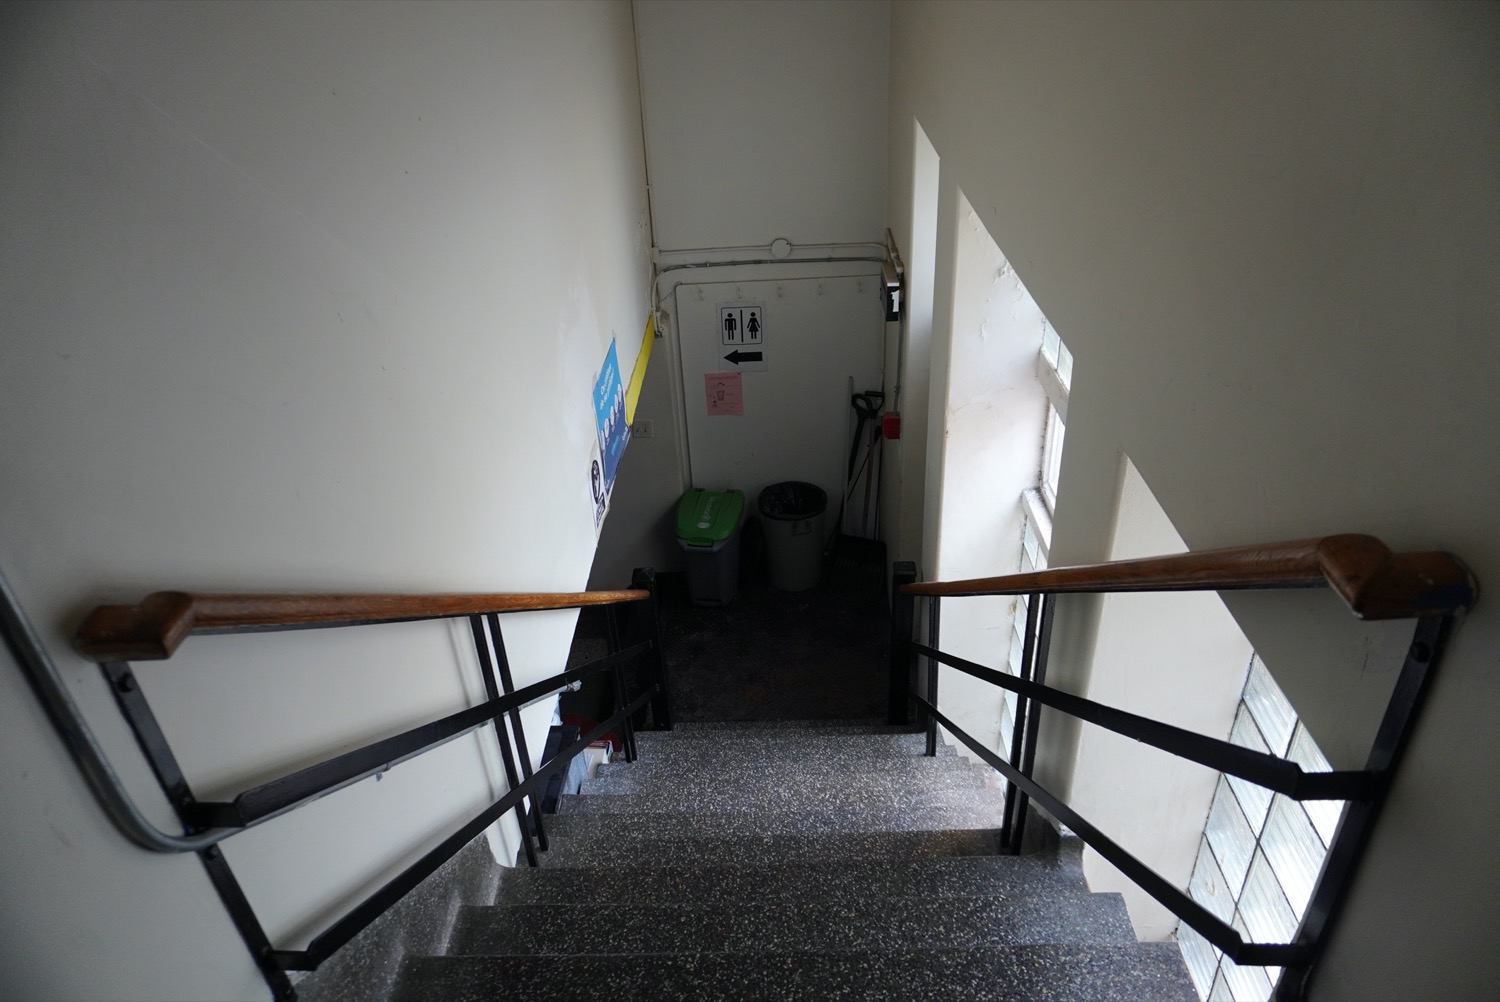
\includegraphics[scale=0.25]{DSC00160.JPG}
    }
    \subfigure{
        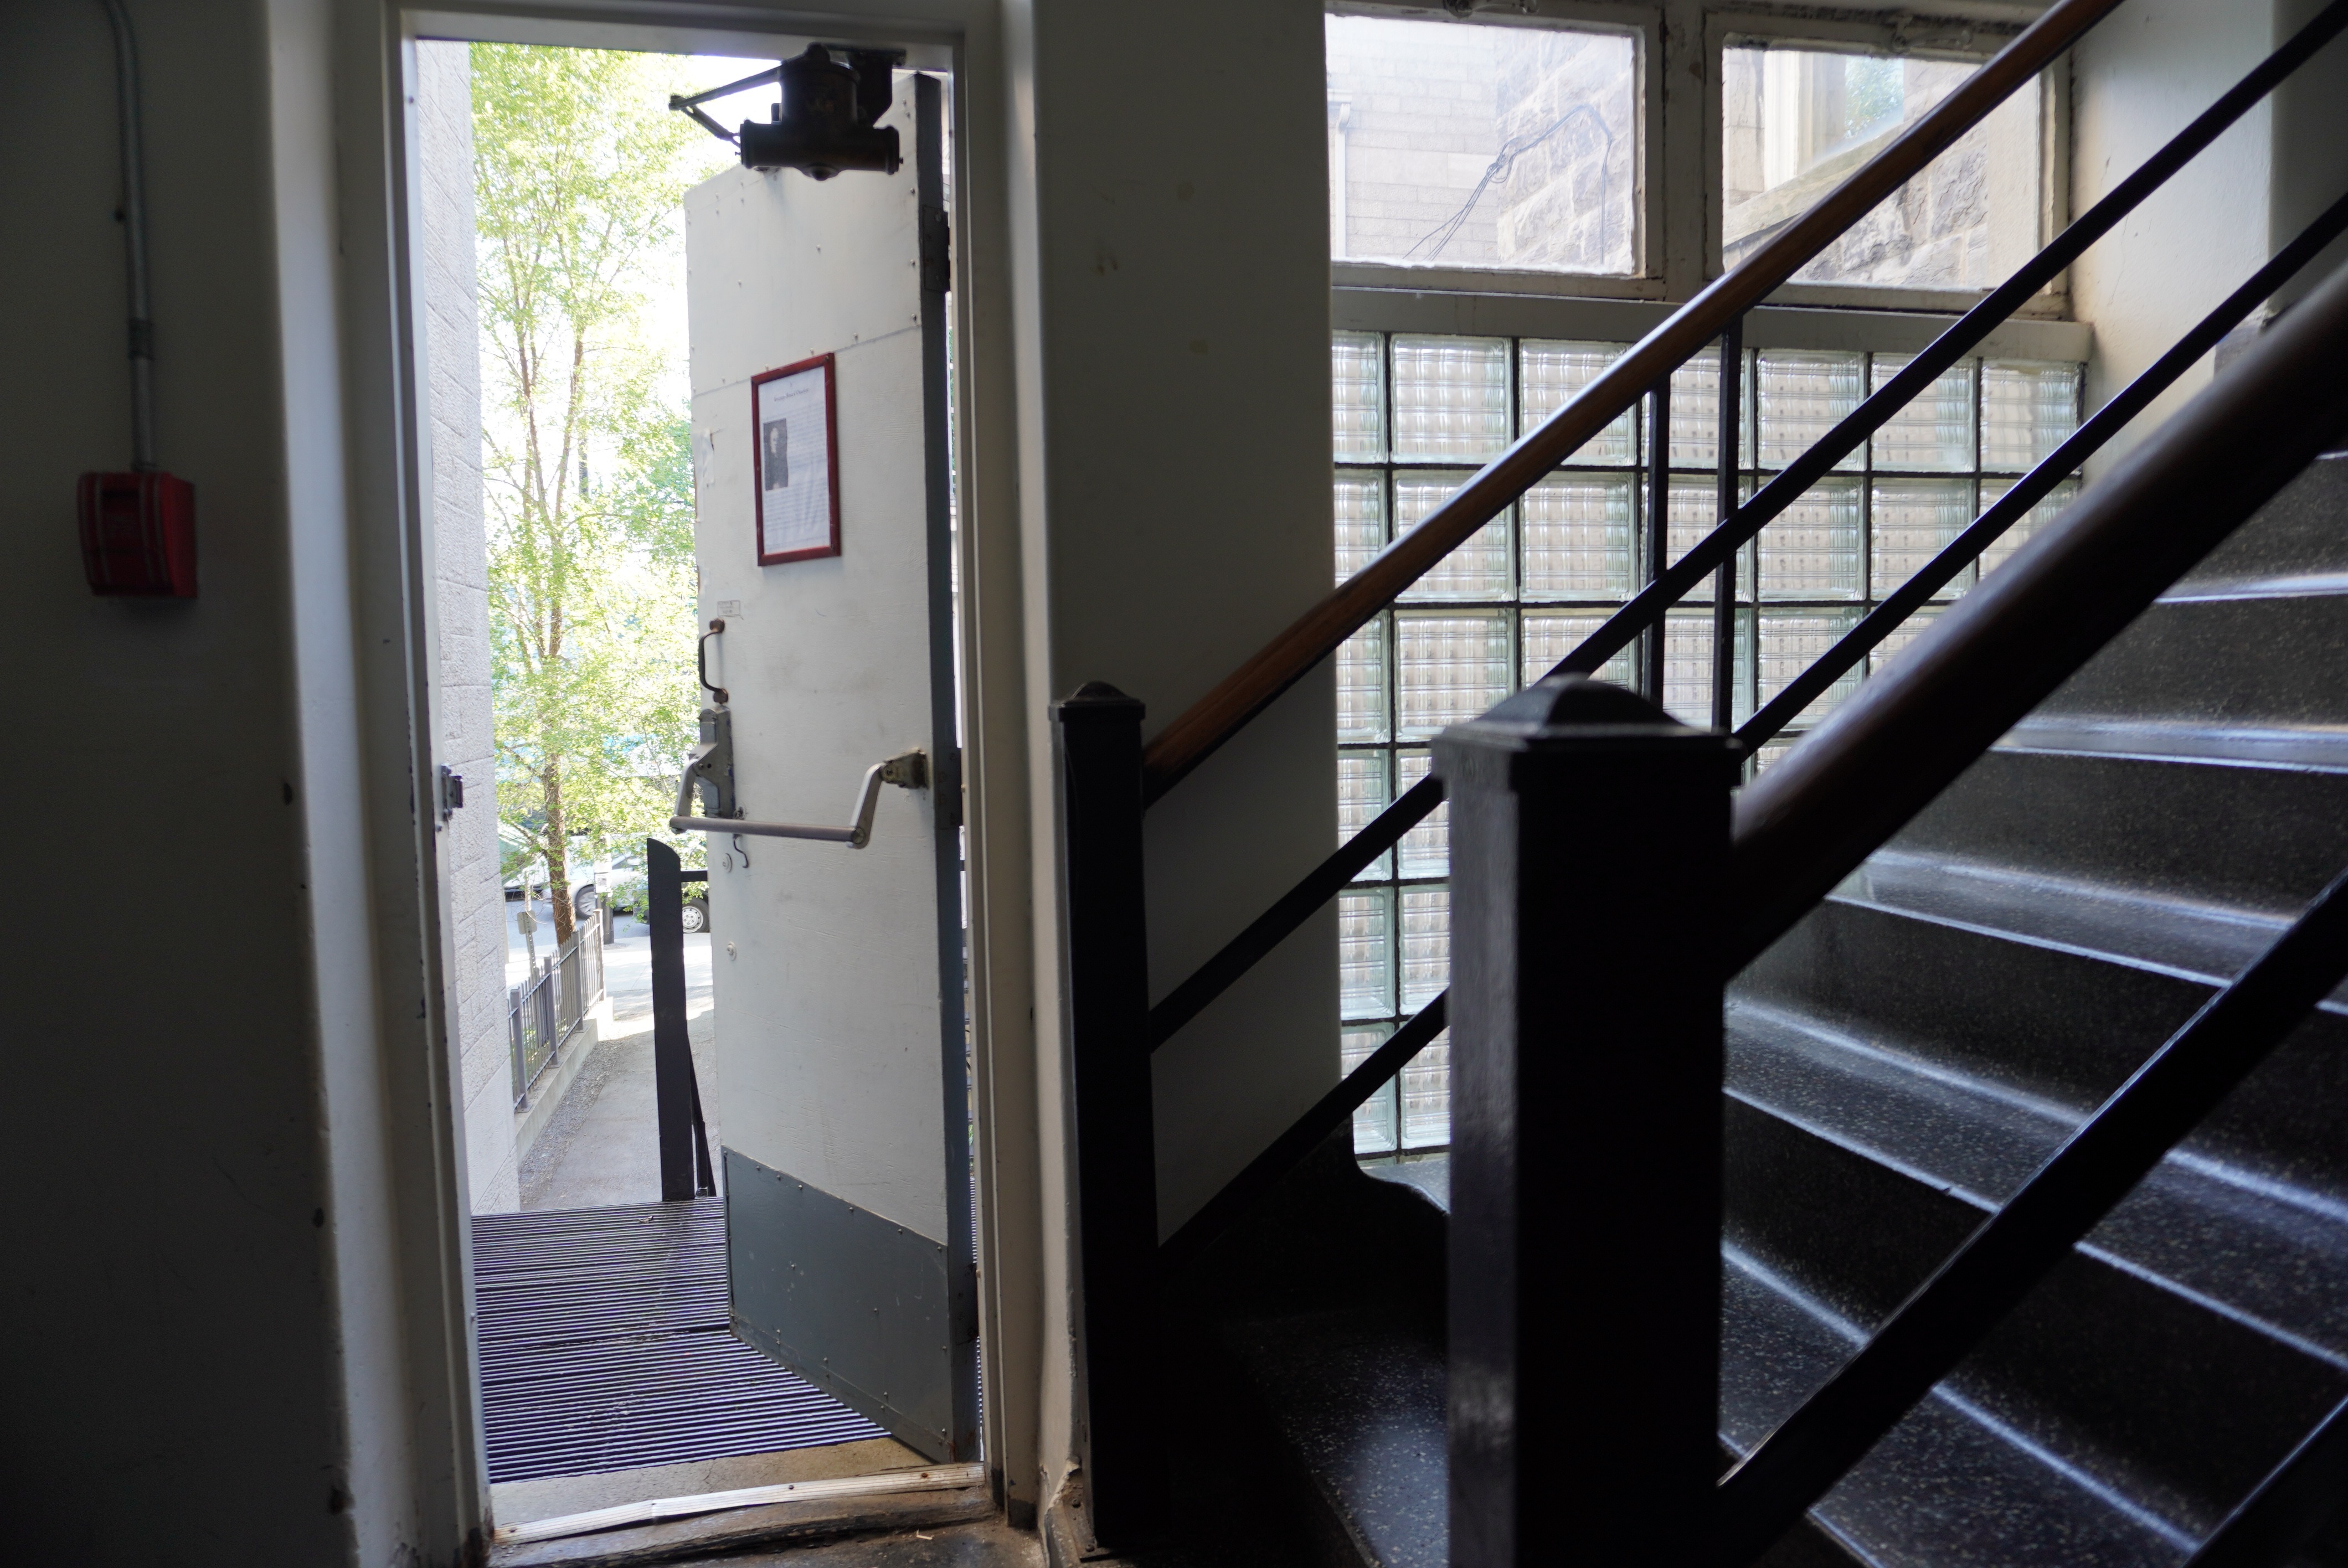
\includegraphics[scale=0.25]{DSC00171.JPG}
    }
    \caption{The door leading from the sacristie to the Chartier hall on the left, and the door leading to the north exit on the right.}
    \label{fig:sidebyside}
\end{figure}

After the initial performances of this piece in April of 2024, I asked several audience members if they had seen these apparitions. 
No one said they had. 
This may seem like a lot of work for it to have been unnoticed, but that I like the idea of leaving subtle surprises in the piece for people that might happen upon them.

The strangeness of these appearances, and the disconnect between the sonic experience and the human form, heighten the sense of disembodiment and tension, parallelling the theme of hauntology and acting as a phantom presence. 
Due to the relatively dark conditions, my identity remains unclear, leading audience members to question whether it is indeed me or someone else, as if the phantom is duplicated, or transported throughout the space.

Once the music sonically reaches the low pulsating drone, I reenter the stage, putting on a lavalier microphone and approaching the organ. 
Although the score marks this as the beginning of the eighth movement, I see it as a liminal space between the seventh and eighth movements—a threshold where the boundaries between the two begin to blur.

\section{\colorbox{red}{8\textsuperscript{e} élégie}\footnote{00:35:35--00:40:23 in elegies\_video.mp4}}

\epigraph{\textit{A plein regards, la créature voit dans l’Ouvert.}}{}

\subsection{Narrative context}

The eighth elegie represents a pivotal moment in \textit{Élégies}, marking a shift from the helplessness and impotence described in the sixth movement to a powerful sense of awakening and transformation. 
The text, "À plein regards, la créature voit dans l’Ouvert," suggests the emergence of something nascent—a being still in the process of becoming. 
I imagine Rilke's creature gradually taking shape, forged from raw potential into a yet unrealized form, as if being called into existence, rather than simply roused from slumber.

This movement occurs after the fully electroacoustic seventh movement, during which the audience has not seen the performer, save for a few apparitions away from the instrument. 
It begins with the organist reentering the audience's view, carrying a flashlight pointed upwards, symbolizing the gradual illumination of this emerging, incomplete being. 
The music mirrors this process, beginning with echoes of earlier motifs and evolving into a complex interplay of live and electroacoustic sounds, symbolizing the creature’s painful yet powerful process of coming into existence.

\subsection{Materials and techniques}

The performer takes their time arriving at the organ, utilizing the looped drone at the end of the seventh elegie—a soundscape characterized by a low rumble and the distant, intermittent sound of a fire alarm. 
This drone loops seamlessly, providing the performer with the necessary space to make registral changes and prepare for the final movements without disrupting the flow of the piece. 
Upon reaching the organ, the performer initiates the 14th trigger, which activates a 3.5-second delay and distortion on the organ sound. 
These effects set the stage for the subsequent echoes and feedback loops, adding tension and anticipation to the music as the performer readies themselves.

The movement begins with soft chords played on the Récit, echoing the parallel stack of fifths heard at the end of the first movement. 
However, after the third iteration, the chords diverge from the original fifths, transitioning into a series of major7 and minor7 chords, mainly in drop 2 4 voicings. 
These chords are echoed across the church, creating a spatial-temporal effect that spans several seconds. 
This echo references the ancient practice of antiphony in Western music and the call-and-response tradition found in various cultures worldwide. 
Poetically, it signifies a broader echo through history, engaging in dialogue with generations past and varied cultures. 
The echoes grow increasingly distorted as they feedback into the system, creating a sense of a dialogue not just across space, but across time and cultural history.

\customincludeexamples[width=\textwidth]{8e_1}{Soft chords harking back to the end of the intial movement mark the performer's return to the instrument (p. 16, sys. 1).}

As the volume and intensity of the chords increase, the music shifts from the Récit to the Positif (with Récit coupled), and finally to the Grand Orgue (with both Récit and Positif coupled). 
The distortion in the echoes becomes more pronounced, and feedback loops begin to form, heightening the sense of chaos. 
At the peak of this intensity, the performer presses the 15th trigger, which stops the creation of new echoes but allows the existing echoes to naturally fade out. 
Following this, the pedal enters with an imposing sound, combining the 32' and 16' flutes with a bright plein orgue registration from the Grand Orgue. 
The resulting sound has an aggressive edge due to its spectral brightness, coupled with a rumbling undertone from the lower registers, creating a powerful, resonant presence that preempts the creature’s emergence.

After six measures of solo pedal, the performer’s hands enter on the Grand Orgue with dissonant chords, each preceded by a rapid triplet figuration, further energizing the distortion. 
The performer then switches to the MIDI keyboard, triggering a sampler based on feedback from the church space itself. 
This feedback was recorded in complete silence, without any input from the organ or voice. 
By gradually raising the gain on a dynamic microphone, the natural room resonance and the noise floor of the microphone were amplified, producing a rich, inharmonic sound. 
Sampling this feedback allows the performer to play different pitches or overlay harmonies, adding an intriguing dimension that is integrally connected to the church acoustics. 
These sampled notes are played between sections of the Grand Orgue, serving as moments of mysterious reflection amid the bursts of intense organ sound.

\customincludeexamples[width=\textwidth]{8e_2}{The entry of the pedal, with coupled plein orgue. At the end of the system is the first entrance of sampled feedback (mm. 1-15).}

After the final section of sampled feedback, where the tension peaks with a dissonant C4 against a D4, the organ suddenly drops out, creating a dramatic silence. 
The performer then triggers the 15th cue, which silences the low rumble of the drone that has persisted since the end of the seventh elegie. 
At this moment, the sound of a match being struck is heard, a callback to the beginning of the seventh movement. 
This signifies the darkness and the need for light, as if the creature is still in the process of emerging, not yet fully formed but on the brink of awakening. 
The crackling match is followed by a rolling, rhythmic sound, gradually growing louder as it moves from the fourth speaker to the first, simulating the passage of a shadow overhead.

As the rolling rhythm reaches a dynamic peak, a loud crack of thunder is heard nearby, marking a dramatic shift. 
A driving beat inspired by UK dubstep rhythms enters, woven from samples of keys, footsteps, and strikes on the pews. 
This rhythm creates the sense that the church itself is participating in an ecstatic dance, introducing a distinctly pop-influenced sound into the piece for the first time. 
Simultaneously, the voice enters with a variation on the falling third motive from the opening vocal gesture, sung in subharmonics to create an eerie, non-human sound. 
This represents the creature as not only something awakening but also something being forged in real-time—a raw, unformed material undergoing a painful process of becoming. 
The vocoder, using the Saint-Édouard bells as a carrier, gradually merges the human voice with the bells, creating a fusion that references the interpolation heard in the third elegie, but now realized in a live, transformative context.

\customincludeexamples[width=\textwidth]{8e_3}{The voice singing subharmonics against the bed track as well as the entry of the bassline over the beat (mm. 31-38).}

\subsection{Theatrical and spatial elements}

The performer’s reentry after the fully electroacoustic seventh movement marks a significant shift in the dramatic tension. 
The slow, deliberate movement towards the organ, flashlight in hand, builds anticipation and a sense of unease, as if the creature is preparing to reveal itself. 
The spatial dynamics, with sounds echoing from across the church, reinforce the idea of a dialogue between different planes of existence, as the creature begins to take form—not just waking up, but being painfully forged into existence.

The echoes and feedback loops play a dual role in this movement. 
On one level, they create a spatial-temporal effect that enhances the immersive experience for the audience. 
On another level, these echoes reference historical musical practices, such as antiphony and call-and-response, symbolizing a dialogue with the past and a connection to broader cultural traditions. 
This historical resonance deepens the thematic exploration of the creature’s transformation, suggesting that its emergence is not just an isolated event but part of a continuum of artistic and spiritual evolution.

The introduction of the beat and the transformation of the voice through subharmonics and vocoding bring the movement to its climax, symbolizing the creature’s full awakening and transformation. 
The dance-like rhythm, juxtaposed with the earlier, more classical and theatrical elements, represents a fusion of the old and the new, the physical and the spiritual. 
The use of church samples in the beat underscores the idea that the church itself is participating in this transformative moment, blurring the lines between the sacred and the profane.

\section{\colorbox{red}{9\textsuperscript{e} élégie}\footnote{00:40:23--00:45:04 in elegies\_video.mp4}}

\epigraph{\textit{Pourquoi, s’il est loisible aussi bien de remplir son délai d’existence en laurier, sombre un peu plus que tous les autres verts, avec ces vaguelettes...}}{}

\subsection{Narrative context}

The ninth elegie is a departure from the patterns established in the previous movements of "Élégies," both in its structure and thematic content. 
This movement begins with text drawn not from the ninth elegie, as one might expect, but from the tenth. 
This choice emerged from a deliberate consideration of how to integrate Rilke’s dense and multifaceted final Elegy into the musical narrative. 
Musically, the tenth Elegy seemed to demand a reflective, non-vocal resolution, serving as a calm after the storm of the preceding movements. 
To maintain the established pattern of incorporating sung lyrics in each movement, the text of the tenth Elegy is instead woven into the fabric of the ninth.

Unlike the other elegies, which each make use of the opening words of Rilke's poems, the lyrics from the 10th Elegy are taken from from various parts of the 10th Elegy. 
This reconstruction is a fragmented mosaic, creating a tapestry of incomplete thoughts and potentialities, mirroring the themes of joy, grief, and longing in Rilke’s poetry. 
This movement, like the text it draws from, grapples with the fear that accompanies happiness--the knowledge that it is transient and inevitably fleeting. 
Musically this movement emerges directly from the eighth, with the beat and baseline that arrive at the end of the previous movement as a link.

\begin{figure}[H]
\begin{verse}
Vienne le jour, enfin sortant.\\ 
La pluie qui vient tomber dans les venelles de la Cité,\\ 
prête à se briser. Mon visage resplendissant, baigné.\\ 
Aux Anges qui l'agréent, des marteaux du cœur.\\
\end{verse}  
\caption{My reconstruction of poetic fragments from Rilke's 10th Elegy} 
\end{figure}

\subsection{Materials and techniques}

The ninth elegie begins as the voice joins the sparse texture of the sample based beat against the baseline in the pedals that ends the eighth Elegy. 
The aesthetic of this section is perhaps the closest to a UK dubstep sound, with the throbbing bass, skittering rhythm, and plaintiff, repetetive vocal line recalling Archangel of Burial. 
The repetitive, plaintive vocal line "Vienne le jour, enfin sortant," sung in D minor, is amplified and processed with a vocoder. 
This technique uses the original church bell sample as the carrier, creating a synthesis between the expressive human voice and the immutable sound of the carillon.

\customincludeexamples[width=\textwidth]{9e_1}{The entrance of the voice over the sparse texture of pedal baseline and sample-based rhythm (mm. 1-8).}

After the initial section, the vocal line drops out, leaving the bassline and beat to carry the momentum for six measures. 
A new idea then emerges in A minor, where the melody of lamentation is transformed from its original 17th-century idiom into a modern, R\&B-inspired expression. 
This transformation is achieved through the use of parallel minor 7 chords and a more pop oriented vocal style. 
The lyrics "La pluie qui vient tomber..." are sung over three iterations of this melody, each iteration progressively higher and more intense, with the organ accompaniment shifting from the positif to the grand orgue.

Following these iterations, the beat is gradually lowered in volume, moving further into the background until it becomes a distant echo, reminiscent of the groanings and clatterings of the church or the city. 
This shift in dynamics allows the organ to take center stage, presenting a solo variation of the "melody of lamentation" in D minor. 
This variation involves a tonicization of G minor, leading into a descending-third, ascending-second sequence, further deepening the sense of unresolved questioning and yearning.

\customincludeexamples[width=\textwidth]{9e_2}{The transition from the second vocal melody into the extended solo organ version with the rhythmic loop in the background (mm. 49-58).}

As the beat fades out, the 17th trigger initiates the sound of rain, taken from the same recording used in the opening of the piece but focused on the rain rather than the thunder. 
The melody of lamentation reappears, this time simplified into a descending diatonic line in augmentation, stretched to one note per measure. 
This is a direct reference to the fourth movement, though the roles of the hands are now reversed: the left hand plays the melody, while the right hand takes up the arpeggiated "spire" motive. 
Over this framework, the voice re-enters, singing an incomplete question to the assenting angels: “Pourquoi, s'il est loisible aussi bien de remplir son délai en laurier. Pourquoi s'il est loisible.”

\customincludeexamples[width=\textwidth]{9e_3}{The lament melody simplified and quantized to whole notes in the left hand, with the arch theme in the right hand, with voice (mm. 79-81).}

\section{\colorbox{red}{10\textsuperscript{e} élégie}\footnote{00:45:04--00:49:13 in elegies\_video.mp4}}

\epigraph{\textit{Vienne le jour enfin, sortant de la voyance encolérée, où je chante la gloire et la jubilation aux Anges qui l’agréent. Que des marteaux du cœur au battement très clair aucun ne vienne à faux tomber sur une corde molle, ou encore douteuse ou prête à se briser.}}{}

\subsection{Narrative context}

The tenth Elegy stands as a contemplative epilogue, a reflective meditation that diverges from the narrative drama of the previous movements. 
This elegie uniquely omits the human voice, a deliberate choice that carries poetic significance. 
The absence indicates otherness--a distance that suggests the elegie is not participating in the unfolding drama but is instead observing, reflecting, and internalizing the previous events. 
This silence points to the idea that the text of the tenth Elegy is not meant to be embodied or expressed outwardly but is rather an internal, imagined experience.

Rilke’s final Elegy grapples with the themes of joy, grief, and the haunting realization that our most profound desires and potentials may remain forever unfulfilled. 
The decision to relegate the text of the tenth Elegy to the ninth movement, where it is fragmented and distorted, introduces a layer of ambiguity. 
This dislocation raises the question of whether the events depicted in the ninth Elegy truly transpired or if they were merely a projection of the protagonist's inner world—a dream of fulfillment that remains just out of reach.

\subsection{Materials and techniques}

The tenth elegie opens with the ethereal sound of reversed bells, immediately setting a reflective tone. 
This is layered with a shimmering plein orgue sound, executed through a two-handed tremolo technique with each hand playing the same chord an octave apart. 
The combination of tremulants and a 50ms delay adds a fluttering, almost dizzying texture that mirrors the swirling thoughts of reflection and introspection. 
Beneath the active surface, the harmonic progression moves slowly, repeating IV-V-I cadences in F major and Ab major. 
This harmonic ambiguity reflects the coexistence of F major and F minor in the spectral composition of the bells.

\customincludeexamples[width=\textwidth]{10e_1}{A tremolo between the two hands, with both tremulant motors active, and a slight delay (mm. 1-9).}

\customincludeexamples[width=\textwidth]{10e_2}{A 6/5 5/3 sequence, followed by the last iteration of the initial theme of the piece (mm. 25-32).}

This section ends with a 6/4 5/3 sequence followed by a final, reharmonized version of the initial theme firs heard in the voice in the first movement. 
The last trigger then turns on a long reverb effect of about 60 seconds which attempts to augment the already significant reverb of the church to something that is essentially frozen in time. 
To represent this timelessness, the notation dissolves into proportional notation, and several frozen, falling by step motives are heard, as the final audio recording is heard: a montage of the sounds of pigeons speaking and fluttering their wings, at first in realtime and gradually slower, combined with a recording of myself coming from the basement of the church and ascending the stairs to the organ loft. 
Because the microphone was placed at the bottom of the stairs to the organ loft, and at the top of the stairs from the basement, my steps are heard approaching the microphone, and then moving into the distance, creating a sense of mystery. 
On the one hand our protagonist has ascended, like the ascension mentioned in the last passage of Rilke's Elegies. 
At the same time, what this ascension represents is unclear.

\customincludeexamples[width=\textwidth]{10e_3}{The final moment of the piece, with a repeated descendng motive with frozen reverb against the sound of pigeons and footsteps (p. 27, sys. 2).}

%%--------------%
%%     index    %
%%--------------%

%% S'il y a lieu, décommenter la ligne pour mettre votre index

%%\printindex

%%------------------------------------------------- %
%%         références --- bibliographie             %
%%------------------------------------------------- %
  % Enlever les commentaires de la prochaine commande si vous préférez que le
  % chapitre s'appelle « Références » plutôt que « Bibliographie » (au choix selon le contexte).
%%\let\bibname=\refname

%% Lorsque vous serez prêt à faire afficher votre bibliographie
%% et vos références, enlevez les commandaires des commandes suivantes
%% et donnez le nom de votre fichier .bib à la commande \bibliography{..}
%% (consultez l'exemple au besoin).  Vous pouvez utiliser le style de votre
%% choix.
%%\bibliographystyle{plain}     % Le style de la bibliographie. Notons que
                                        % les extensions ne sont pas données pour ces deux fichiers.
%%\def\bibname{R\'ef\'erences bibliographiques} % Nom obligatoire de la section des références.
                                              % On utilise \'e car le é cause des problèmes
                                              % dans la table des matière
%% ENGLISH
%%\def\bibname{References}
\printbibliography
%%\bibliography{ref}     % La base de données contenant des entrées bibliographiques.
                                    % Seules celles référencées dans le texte seront ajoutées
                                    % \`a la bibliographie.

%%------------------------------------------------- %
%%                  Annexe A                        %
%%------------------------------------------------- %

\appendix
\chapter{List of digital and audiovisual documents on DVD}

%%\section{test}

\begin{itemize}
    \setlength\itemsep{0.5em}  % Adjust space between items if needed
    \setlength\parskip{0pt}    % Ensure no extra spacing between paragraphs
    \setlength\parsep{0pt}
    \setlength\leftskip{0pt}   % Remove any global indentation
    \setlength{\labelsep}{0pt} % Remove space between label and text
    \renewcommand{\labelitemi}{} % Remove the bullet point
    \renewcommand{\labelitemii}{} % Remove nested bullet points if needed

    \item \hangindent=2em \textbf{thesis.pdf}
    \par Digital version of the thesis.
     
    \item \hangindent=2em \textbf{elegies\_score.pdf}
    \par Score for Élégies.
    
    \item \hangindent=2em \textbf{elegies\_audio.wav}
    \par Edited audio combining April 26, 2024 and April 28, 2024 performances of Élégies.
    
    \item \hangindent=2em \textbf{elegies\_video.mp4}
    \par Video from April 28, 2024 performance of Élégies.
    
    \item \hangindent=2em \textbf{synthesis\_demo.mp4}
    \par A short demo of synthesis effects used in Élégies. Created for the Y6 ACTOR conference in Vancouver in July, 2024.
    
    \item \hangindent=2em \textbf{effects\_demo.mp4}
    \par A short demo of live effects processing used in Élégies. Created for the Y6 ACTOR conference in Vancouver in July, 2024.

    \item \hangindent=2em \textbf{jardin\_de\_givre\_score.pdf}
    \par Score for Jardin de givre.
    
    \item \hangindent=2em \textbf{jardin\_de\_givre\_video.mp4}
    \par Video from April 2023 performance of Jardin de givre.
\end{itemize}

%%\chapter{Les différentes parties et leur ordre d'apparition}

%%J'ajoute ici les différentes parties d'un mémoire ou d'une thèse ainsi
%%que leur ordre d'apparition tel que décrit dans le guide de
%%présentation des mémoires et des thèses de la Faculté des études
%%supérieures.  Pour plus d'information, consultez le guide sur le site
%%web de la facutlé (www.fes.umontreal.ca).

%%\newcount\colnum
%%\colnum=1
%%\def\i{\number\colnum. \global\advance\colnum by 1\ignorespaces}
%%\begin{table}[p]
%%  \begin{center}
%%    \begin{tabular}{|l|l|r|}\hline
%%       \noindent\hfil
%%         \textbf{\strut Ordre des éléments constitutifs du mémoire ou de la thèse}
%%         \hfil\span\omit\span\omit\\\hline % \span\omit pour couvrir plus d'une
%%                                           % case sans utiliser le package multirow ou autre
%%      \i &  La page de titre & obligatoire\\\hline
%%      \i &  La page d'identification des membres du jury & obligatoire\\\hline
%%      \i &  Le résumé en français et les mots clés français\kern3em& obligatoires\\\hline
%%      \i &  Le résumé en anglais et les mots clés anglais & obligatoires\\\hline
%%      \i &  Le résumé dans une autre langue que l'anglais & obligatoire \\
%%         &  ou le français (si le document est écrit dans &\\
%%         &  une autre langue que l'anglais ou le français)&\\\hline
%%      \i &  Le résumé de vulgarisation& facultatif\\\hline
%%      \i &  La table des matières, la liste des tableaux,& obligatoires\\
%%         &   la liste des figures ou autre &\\\hline
%%      \i &  La liste des sigles et des abréviations& obligatoire\\\hline
%%      \i &  La dédicace& facultative\\\hline
%%      \i &  Les remerciements & facultatifs\\\hline
%%      \i &  L'avant-propos & facultatif\\\hline
%%      \i &  Le corps de l'ouvrage& obligatoire\\\hline
%%      \i &  Les index& facultatif\\\hline
%%      \i &  Les références bibliographiques & obligatoires\\\hline
%%      \i &  Les annexes & facultatifs\\\hline
%%      \i &  Les documents spéciaux & facultatifs\\\hline
%%    \end{tabular}
%%  \end{center}
%%\end{table}

\end{document}

\endinput
%%
%% End of file `gabaritmem.tex'.
